\documentclass[10pt,a4paper,openright]{report}

\usepackage[width=15.00cm, height=23.00cm]{geometry}
\usepackage[italian]{babel}
\usepackage[utf8]{inputenc}
\usepackage[T1]{fontenc}
\usepackage{dsfont}
\usepackage{amsmath}
\usepackage{amsfonts}
\usepackage{amssymb}
\usepackage{graphicx}
\usepackage{paracol}
\usepackage{xparse}
\usepackage{sidecap}
\usepackage[makeroom]{cancel}
\usepackage{capt-of}
\usepackage{caption}
\usepackage[dvipsnames]{xcolor}
\usepackage{xpatch}
\usepackage{subcaption}
\usepackage[most]{tcolorbox}
\usepackage{lipsum}
\usepackage{float}
\usepackage{imakeidx}
\usepackage{wrapfig}
\usepackage{marginnote}
\usepackage{ upgreek }
\usepackage{bm}
\usepackage{enumerate}
\usepackage{tickzit}
\usepackage{ mathrsfs }

\input{stilifigure.tikzstyles}
\graphicspath{{Immagini/}}

%\newcommand{\de}[1]{\textbf{\textcolor{NavyBlue}{#1}}}

\makeindex[columns=3, title=Indice Analitico, intoc]

\captionsetup{font = {it, small}, labelfont={color=NavyBlue, bf}}


\renewcommand{\H}{\mathcal H}
\renewcommand{\S}{\mathcal S}
\newcommand{\F}{\mathcal F}
\newcommand{\E}{\mathcal E}
\newcommand{\R}{\mathcal R}
\newcommand{\I}{\mathcal I}
\renewcommand{\L}{\mathscr L}
\newcommand{\aL}{\mathscr {L}^{-1} }
\newcommand{\trasf}[1]{\mathscr L \left( #1 \right)}
\newcommand{\anti}[1]{\mathscr {L}^{-1} \left( #1 \right) }
\newcommand{\C}{\mathcal C}
\newcommand{\D}{\mathcal D}
\newcommand{\scal}{\textrm{scal}}
\newcommand{\ramp}{\textrm{ramp}}
\newcommand{\imp}{\textrm{imp}}


\newcommand{\ov}[1]{ \vett{#1}  	}
\newcommand{\vers}[1]{ \boldsymbol{\hat{#1}}  	}
\newcommand{\vett}[1]{ \boldsymbol{#1}  	}
\newcommand{\dov}[1]{ \dot{\boldsymbol{#1}  }	}
\newcommand{\pd}[2]{\frac{\partial #1}{\partial #2}}



\newcommand{\opdiff}{\Big[\ \partial \ \Big] }
\newcommand{\matalpha}{\Big[\ \alpha \ \Big] } 
\newcommand{\asmat}[1]{ \big[ \ #1 \ \big] }

\newcommand{\figura}[5]{\begin{SCfigure}[#2][b!h!t!]
		\centering
		\includegraphics[width=#1 cm]{#3}
		\caption{#4} \label{#5}
\end{SCfigure}}


\newcommand{\figuratikz}[5]{\begin{SCfigure}[#2][b!h!t!]
\centering
\resizebox{#1cm}{!}{\tikzfig{Immagini/#3}}
\caption{#4} \label{#5}
\end{SCfigure}}

\newcommand{\matrice}[1]{\begin{bmatrix} #1 \end{bmatrix}}













\newcommand{\bfcolor}[1]{\renewcommand*{\textbf}[1]{{\bfseries{\color{#1}##1}}}}

\setcolumnwidth{0.3\textwidth}



\newcounter{concetti}
\newenvironment{concetto}{
	
	\bfcolor{NavyBlue}
	\refstepcounter{concetti}
	{\color{NavyBlue}\textbf{Concetto \theconcetti: }} 
}{
}
\numberwithin{concetti}{chapter}
\tcolorboxenvironment{concetto}{
	boxrule=0pt,
	boxsep=0pt,
	colback={White!90!NavyBlue},
	enhanced jigsaw, 
	borderline west={2pt}{0pt}{NavyBlue},
	sharp corners,
	before skip=5pt,
	after skip=10pt,
	breakable,
}

\newcounter{teoremi}
\newenvironment{teorema}[2]{
	\bfcolor{ForestGreen}
	\refstepcounter{teoremi}
	\textbf{Concetto \theteoremi #1} 
	\vspace{3mm} 
	
	\texttt{Ipotesi: } #2
	
	\vspace{3mm} 
	
	\texttt{Enunciato}: 
}{
}
\numberwithin{teoremi}{chapter}
\tcolorboxenvironment{teorema}{
	boxrule=0pt,
	boxsep=0pt,
	colback={White!100!ForestGreen},
	enhanced jigsaw, 
	borderline west={2pt}{0pt}{ForestGreen},
	sharp corners,
	before skip=5pt,
	after skip=10pt,
	breakable,
}


\newenvironment{dimostrazione}{
	\bfcolor{Orchid}
	\textbf{Dimostrazione} \quad
}{ }
\tcolorboxenvironment{dimostrazione}{
	boxrule=0pt,
	boxsep=0pt,
	colback={White!100!NavyBlue},
	enhanced jigsaw, 
	borderline west={2pt}{0pt}{Orchid},
	sharp corners,
	before skip=5pt,
	after skip=10pt,
	breakable,
}

\newenvironment{osservazione}{
	\bfcolor{BurntOrange}
	\textbf{Osservazione: }
}{ }
\tcolorboxenvironment{osservazione}{
	boxrule=0pt,
	boxsep=0pt,
	colback={White!100!BurntOrange},
	enhanced jigsaw, 
	borderline west={2pt}{0pt}{BurntOrange},
	sharp corners,
	before skip=5pt,
	after skip=10pt,
	breakable,
}

\newenvironment{nota}{
	\bfcolor{CadetBlue}
	\textbf{Nota: }
}{ }
\tcolorboxenvironment{nota}{
	boxrule=0pt,
	boxsep=0pt,
	colback={White!100!CadetBlue},
	enhanced jigsaw, 
	borderline west={2pt}{0pt}{CadetBlue},
	sharp corners,
	before skip=5pt,
	after skip=10pt,
	breakable,
}




\newcounter{numrichiamo}
\newenvironment{richiamo}{
	\noindent
	\refstepcounter{numrichiamo}
	
%	\renewcommand{\de}[1]{ { \color{ForestGreen} \textbf{#1} } }
	
	{\color{ForestGreen}\textbf{Richiamo \thenumrichiamo:}}
}{
}
\tcolorboxenvironment{richiamo}{
	boxrule=0pt,
	boxsep=0pt,
	colback={White!90!ForestGreen},
	enhanced jigsaw, 
	borderline west={2pt}{0pt}{ForestGreen},
	sharp corners,
	before skip=5pt,
	after skip=5pt,
	breakable,
}

\newcounter{esempi}
\numberwithin{esempi}{chapter}
\newenvironment{esempio}[1]{
	\bfcolor{Periwinkle}
	\noindent
	\refstepcounter{esempi}
	{\color{Periwinkle}\textbf{Esempio \theesempi#1}  } 
	\vspace{3mm}
	
	\noindent
}{
}


\tcolorboxenvironment{esempio}{
	boxrule=0pt,
	boxsep=0pt,
	colback={White!90!Periwinkle},
	enhanced jigsaw, 
	borderline west={2pt}{0pt}{Periwinkle},
	sharp corners,
	before skip=10pt,
	after skip=10pt,
	breakable,
}


\usetikzlibrary{arrows.meta}


\begin{document}
	\pagenumbering{roman}
	
	\makeatletter
	\begin{center}
		\vspace{3cm}
		\thispagestyle{empty}
		$ \quad $
		
		\vspace{1.5cm}
		
		
\includegraphics[width=5cm]{logouni}
		
		\vspace{2cm}
		
		{\Large Università degli Studi di Trento}
		
		\vspace{2cm}
		{\Large Dipartimento di Ingegneria Industriale} \\ \vspace{2mm}
		{\LARGE \textbf{Corso di Fondamenti di Automatica}} \\ \vspace{2mm}
		{\Large Docente: Panzani Giulio}\\
		\texttt{giulio.panzani@studenti.unitn.it}
		
		\vspace{2cm}
		{\LARGE \textbf{Appunti del corso}}
		
		\vspace{2cm}
		{\large 
			Matteo Dalle Vedove \\
			matteo.dallevedove@studenti.unitn.it
			
			\vspace{2cm}
			Anno Accademico 2020-2021 \\ 28 gennaio 2021}
	\end{center}
	
	\tableofcontents
	
	
	\pagenumbering{arabic}
	\chapter{Automatica e sistemi}

	\begin{concetto}
		\textit{L'\textbf{automatica} è la disciplina che studia come agire su un sistema in modo che il suo comportamento assomigli a quello desiderato, senza necessità  di intervento manuale}.
	\end{concetto}
	Di fatto lo scopo di questo corso è quello di capire come un sistema da controllare si comporta e studiare un opportuno controllore in grado da fornire dei risultati accettabili.
	
\section{Sistema di controllo}
	\subsection{Sistema}
	
		\begin{concetto}
			L'automatica si basa sullo studio di \textbf{sistemi}, ossia un insieme di elementi fisici o concettuali il cui comportamento cambia nel tempo e/o spazio e che interagiscono con il mondo circostante. I sistemi, come mostrati in figura \ref{sistema}, sono modellati come delle \textit{black box} le cui interazioni con l'ambiente esterno sono rappresentate dai rami, ossia le frecce entranti/uscenti: in particolare si osservano
			\begin{itemize}
			    \item gli \textbf{ingressi di controllo}  $u$ (o semplicemente \textbf{ingressi}) i valori in ingresso al sistema che potranno essere modificati a piacimento dal controllore;
			    \item gli \textbf{ingressi di disturbo} $d$, ossia valori la cui evoluzione non può essere influenzata e in generale dei quali non è conosciuto l'andamento;
			    \item le \textbf{uscite} $y$ del sistema che descrivono la sua evoluzione e che dunque possono influenzare l'ambiente con il quale interagiscono.
			\end{itemize}
		\end{concetto}

    	\figuratikz{4}{1}{sistema}{schema di un sistema.}{sistema}
    	
    	In molti casi la scelta di catalogare una variabile come ingresso o uscita è puramente arbitraria e deve essere contestualizzata al problema da risolvere. Considerando l'esempio di un'automobile, la coppia motrice può essere considerata come un'uscita se si considera che essa derivata dal motore che si interfaccia sul veicolo e che è determinata da ingressi quali la quantità di carburante, temperatura dell'aria ecc. Tuttavia la stessa coppia motrice può anche essere considerata come un ingresso che l'automobile utilizza per seguire la sua traiettoria.
    	
    \subsection{Controllo}
        \begin{concetto}
                Il \textbf{controllore} è la \textit{black box} che rappresenta il controllo automatico, ossia che descrive l'azione che deve essere applicata al sistema per farlo evolvere come desiderato. Il controllore, mostrato in figura \ref{controllore}, è del tutto similare come rappresentazione ad un sistema, dove tuttavia come rami in ingresso si osserva la \textbf{specifica del problema} $\overline y$, ossia il valore di \textbf{riferimento} al quale deve tendere a regime il sistema, mentre in uscita si ha l'\textbf{azione di controllo} $u$ del controllore $C$ sul sistema $S$. Altri ingressi sono connotati generalmente dalla variabile $i$.
         \end{concetto}
    	
    	\figuratikz{4}{1}{controllo}{schema di un controllore.}{controllore}
    	
    	Idealmente la \textbf{variabile controllata} (ossia l'uscita $y$ del sistema $S$) deve essere pari al segnale di riferimento $\overline y$ in ogni condizione, ossia indipendentemente dal rumore $n$ e dai disturbi $d$ che agiscono sull'insieme di controllore e sistema. Tuttavia per modellare più \textit{correttamente} l'andamento reale in generale l'obbiettivo del controllo è quello di minimizzare l'errore $e$ del sistema:
    	\begin{equation}
    	    \underbrace{\textrm{errore}}_e = \underbrace{\textrm{valore di riferimento}}_{\overline y} - \underbrace{\textrm{variabile controllata}}_y
    	\end{equation}
    	
    	Spesso i limiti delle specifiche di controllo sono limitate dalla grandezza della variabile di controllo stessa: per esempio una Fiat non potrà mai accelerare come una Ferrari per via del motore che è implementato sulla stessa.
    	
    \subsection{Sistema di controllo} \label{sec:sistemacontrollo}
        \begin{concetto}
            Un opportuno collegamento tra controllore $C$ e sistema $S$ determina dunque il \textbf{sistema di controllo} (figura \ref{fig:sis:anelli}); questo nuovo sistema contiene praticamente tutti gli elementi fin'ora visti, ossia in particolare il valore di riferimento $\overline y$, la variabile di controllo $u$ che si interfaccia sul sistema e l'uscita $y$ del sistema, ossia la \textbf{variabile da controllare}.
            
            E' inoltre possibile classificare i sistemi di controllo in base alla topologia degli stessi, in particolare si parla di \textbf{anello aperto} quando le uscite del sistema $y$ non sono poste in retroazione alla variabile di riferimento, mentre quando ciò avviene si parla di controllo in \textbf{anello chiuso}.
        \end{concetto}
        
        \begin{figure}[bht]
        	\centering 
        	\begin{subfigure}{0.48\linewidth}
        		\centering
        		\resizebox{0.98\linewidth}{!}{\tikzfig{Immagini/sistema-controllo-a}} \caption{}
        	\end{subfigure}
	        \begin{subfigure}{0.48\linewidth}
		        \centering
		        \resizebox{0.98\linewidth}{!}{\tikzfig{Immagini/sistema-controllo-b}} \caption{}
		    \end{subfigure}
	    	\caption{esempio di sistema di controllo in anello aperto (a) e in anello chiuso (b).}
	    	\label{fig:sis:anelli}
        \end{figure}
            	
        Come si osserverà un sistema in anello aperto per poter funzionare \textit{correttamente} deve conoscere perfettamente il funzionamento del sistema e i parametri dello stesso, mentre un sistema in anello chiuso, seppur più complesso (in quanto prevede il montaggio di sensori e algoritmo di controllo più sofisticati), permette di ottenere prestazioni sensibilmente \textit{migliori}, immuni da incertezze e interferenze esterne.
    	
    	\begin{concetto}
    		Il \textbf{problema di controllo} è quello dunque di determinare le variabili di controllo $u$ affinché le variabili da controllare siano simili al segnale di riferimento per ogni possibile \textit{traiettoria} del riferimento $\overline y$ e dei disturbi $d$:
    		\[ y\simeq \overline y \]
    	\end{concetto}
    
\section{Classificazione dei sistemi}
	Come fin'ora visto, i sistemi (e i controlli) possono essere assimilati a delle black box caratterizzate dagli ingressi $u$ e le uscite $y$. In un sistema è possibile individuare sia deii \textbf{parametri}, ossia delle quantità che descrivono la struttura e le proprietà del sistema (come la massa o la geometria di un corpo) che tendenzialmente sono tempo-invarianti, sia delle \textbf{variabili}, ossia delle grandezze che descrivono l'evoluzione nel tempo del sistema (come posizione e velocità del corpo).
	
	A questo punto è dunque fondamentale \textbf{classificare} i vari sistemi nei cosiddetti \textit{\textbf{assi di classificazione}}, ossia una serie di connotazioni non esclusive che permettono di categorizzare i vari tipi di sistemi.
	
	\subsubsection{MIMO e SISO}
		Questo asse di classificazione è caratterizzato dagli acronimi \textit{Multi-Input Multi-Output} MIMO e \textit{Single-Input Single-Output} SISO; come si può evincere dalla traduzione dall'inglese, un sistema MIMO presenta un numero multiplo sia di ingressi $u$ che di uscite $y$ e dunque tali valori possono essere rappresentati da un vettore. Al contrario un sistema SISO presenta un solo valore in ingresso $u$ e un'uscita $y$, e dunque possono essere descritti solamente da un valore scalare.
		
		In particolare le $n$ uscite di un sistema MIMO sono collegate agli $m$ ingressi dello stesso secondo delle relazioni funzionali $f_i$ secondo che possono essere espresse come
		\begin{align*}
			y_1 & = f_1\big(u_1, u_2,\dots, u_m\big) \\
			y_2 & = f_2\big(u_1, u_2,\dots, u_m\big) \\
			& \ \vdots \\
			y_n & = f_n\big(u_1, u_2,\dots, u_m\big) 
		\end{align*}
	
	\subsubsection{Sistemi lineari e non lineari}
		Un \textbf{sistema} è detto \textbf{lineare} se rispetta le condizioni di linearità tra ingresso e uscita, ossia se nota l'uscita $f(u_1), f(u_2)$ per due ingressi noti $u_1,u_2$, allora l'uscita $f(u)$ di un ingresso ottenuto come combinazione lineare di $u_1,u_2$ deve essere la stessa combinazione lineare delle due uscite; in termini matematici una funzione per essere lineare deve essere tale che
		\[ u = \alpha_1 u_1 + \alpha_2 u_2 \qquad \Rightarrow \quad f(u) = \alpha_1 f(u_1) + \alpha_2 f(u_2) \]
    	Ogni qualvolta questa condizione non venisse rispettata, il \textbf{sistema} è semplicemente detto \textbf{non lineare}.
    
    	\paragraph{Rappresentazione matriciale per sistemi lineari} In generale un sistema lineare di tipo mimo può essere espresso come un sistema di equazioni lineari del tipo
    	\[\begin{cases}
    		y_1 = k_{11} u_1 + \dots + k_{1m} u_m \\
    		\ \vdots \\ 
    		y_n = k_{n1} u_1 + \dots + k_{nm} u_m
    	\end{cases}\]
    	Per come visto in algebra lineare è altresì possibile convertire tale sistema in \textit{notazione algebrica} in un sistema rappresentato in forma matriciale dal vettore $\boldsymbol u$ degli ingressi e $\boldsymbol y$ delle uscite e dalla matrice dei coefficienti $ K$:
    	\[ \boldsymbol{y} = K \boldsymbol{u} \qquad \leftrightarrow\qquad \begin{pmatrix}
    		y_1 \\ \vdots \\ y_n
    	\end{pmatrix} = \begin{bmatrix}
    		k_{11} & \dots & k_{1m} \\ 
    		\vdots & \ddots \\
    		k_{n1} & & k_{nm}
    	\end{bmatrix} \begin{pmatrix}
    		u_1 \\ \vdots \\ u_m
    	\end{pmatrix}\]
    	\begin{osservazione}
    		In seguito non verrà più rappresentata alcuna differenza tra la rappresentazione degli ingressi $u$ e uscite $y$ come scalari o vettori, in quanto i due comportamenti per sistemi lineari sono analoghi.
    	\end{osservazione}
    	
    \subsubsection{Sistemi a tempo continuo e a tempo discreto}
    	Nei \textbf{sistemi a tempo continuo} le variabili evolvo, per l'appunto, con continuità nel tempo $t$, mentre i \textbf{sistemi a tempo discreto} presentano variabili che mutano solamente in corrispondenza di tempi $k\in \mathds Z$ che possono assumere solamente valori discreti interi.
    	
    	In generale i sistemi a tempo discreto derivano o dall'approssimazione di sistemi a tempo continuo oppure da sistemi dinamici (tendenzialmente concettuali) che nativamente devono prevedere una successione di eventi ad intervalli (come per esempio un algoritmo di calcolo di zeri di funzione tramite il metodo di Newton).
    	
    \subsubsection{Sistemi tempo varianti e tempo invarianti}
    	Sono detti \textbf{sistemi tempo varianti} tutti quei sistemi per cui il funzionale $f$ che lega l'uscita con l'ingresso dipende esplicitamente dal tempo, ossia assume una \textit{forma} del tipo
    	\[  y = f(u,t)\]
    	Un esempio di questo tipo di sistema è dato dalla funzione $f(u,t) = u^2 + 2t$.
    	
    	Al contrario se la funzione $f$ è indipendente dal tempo $t$, allora il \textbf{sistema} è detto \textbf{tempo invariante} ed è rappresentato da una relazione del tipo
    	\[ y = f(u) \]
    	Un esempio di questo tipo di sistema è dato dalla relazione $f(u) = e^u + 2u^3$.
    	
    	\begin{osservazione}
    		La (in)varianza del sistema rispetto al tempo è riferita solamente rispetto al funzionale $f$ che lega in generale l'ingresso con l'uscita, ma non all'ingresso $u$ che può variare nel tempo per stabilire la \textit{dinamica} del sistema!
    	\end{osservazione}
    
   	\subsubsection{Sistemi statici e sistemi dinamici}
   		La distinzione tra sistemi statici e dinamici è la più importante in quanto ci permette di capire meglio come approcciare l'analisi del sistema.
    	
    	\begin{concetto}
    		Un \textbf{sistema} è detto \textbf{statico} se la relazione tra ingresso è uscita è descritta da un'equazione algebrica del tipo $$y=f(u)$$
    		Intuitivamente ciò significa che per determinare l'uscita $y$ ad un istante generico di tempo $t^*$ è sufficiente conoscere il valore dell'ingresso $u^*$ in tale istante: in questo modo la \textit{storia} degli ingressi è ininfluente sulla determinazione dell'uscita e per questo tali sistemi sono detti \textbf{\textit{memory-less}}.
    	\end{concetto}
    	\begin{concetto}
    		Al contrario di quanto appena affermato, sono detti \textbf{sistemi dinamici} tutti quei sistemi rispetto ai quali per determinare il valore dell'uscita $y$ al tempo $t^*$ non è sufficiente conoscere solamente l'ingresso $u(t^*)$, ma anche tutto il pregresso temporale dell'ingresso $u(t)$ nell'intervallo di tempo compreso tra l'origine dei tempi $t_0$ e il tempo in questione $t^*$. Matematicamente questo tipo di sistemi è dunque governato non da un'equazione algebrica ma da un'\textbf{equazione differenziale} (ordinarie).
    		
    		Per questi sistemi sono dette \textbf{variabili di stato}, generalmente indicate come $x$, quelle variabili che occorre conoscere all'istante $t_0$ (insieme alla storia degli ingressi $u(t)$) per determinare univocamente l'uscita $y(t^*)$.
    	\end{concetto}
    
    	\begin{esempio}{: bottiglia che si riempie} \label{es:intro:bottiglia}
    		Si consideri il caso di una bottiglia (approssimata ad un cilindro) nella quale si versa una portata d'acqua $q$ (corrispondente all'ingresso $u$ del sistema) alla quale è associata la quota $h$ di fluido (corrispondente all'uscita del sistema) nella bottiglia stessa.
    		
    		In questo caso la \textbf{variabile di controllo} corrisponde alla portata $q=u$ (ingresso), mentre la \textbf{variabile controllata} è la quota $h = y$.
    		\begin{center}
    			\tikzfig{Immagini/bottiglia}
    		\end{center}
    		Osservando l'andamento dell'ingresso $u$ del sistema (diagramma a sinistra), è possibile osservare come nel tempo il livello del fluido (uscita $y$) vari nel tempo (diagramma a destra).
    		
    		Questo esempio ci permette di capire che il \textbf{sistema} è \textbf{dinamico}; considerando per esempio gli istanti $t_1,t_2$, dal diagramma a sinistra è possibile osservare che gli ingressi sono uguali e pari a zero (non si ha flusso di acqua entrante nella bottiglia), tuttavia il livello di acqua nei due istanti è diverso per via del fatto che nell'intervallo di tempo $[t_a,t_b]$ si ha avuto un flusso di acqua entrante nel sistema che ha cambiato il livello di fluido nella bottiglia.
    	\end{esempio}
    
\section{Spazio di stato e sua rappresentazione} \label{sec:intro:spaziostato}
	\begin{concetto}
		La \textit{metodologia universale} per descrivere i sistemi dinamici è basata sulla \textbf{rappresentazione in spazio di stato} del sistema stesso. Questa metodologia si basa sulla scrittura di una serie di \textbf{equazioni di stato} $f$ che relazionano la derivata prima $\dot x$ di una variabile di stato con le variabili di stato (non derivate), gli ingressi e il tempo secondo delle relazioni del tipo
		\[ \dot x = f( x,u,t)\]
		Per completare la rappresentazione è inoltre necessario scrivere anche le \textbf{trasformazioni d'uscita} $g$ che legano le uscite $y$ con le variabili di stato, gli ingressi e il tempo con una relazione del tipo
		\[ y = g(x,u,t)  \]
	\end{concetto}
	\begin{osservazione}
		Se il sistema prevede $n$ variabili di stato, allora sarà necessario scrivere un numero uguale di equazioni di stato $f_i$, una per ogni variabile. In modo analogo in presenza di $m$ uscite del sistema, sarà necessario determinare altrettante trasformazioni. Il tutto si basa sul fatto che $u,x,y$ possono rappresentare dei vettori ma anche degli scalari.
	\end{osservazione}
	Noto il numero $n$ di equazioni differenziali che è possibile individuare in un sistema dinamico, allora tale numero prende il nome di \textbf{ordine del sistema} e rappresenta il numero di variabili di stato $x$ che devono essere utilizzate nell'analisi per descrivere completamente il sistema stesso.
	
	\begin{esempio}{: rappresentazione in spazio di stato} \label{es:intro:bottiglia-2}
		Facendo riferimento all'esempio \ref{es:intro:bottiglia} della bottiglia che si riempie, è possibile creare un modello matematico del sistema. Nota infatti l'area $A$ della base del cilindro, l'altezza $h$ del fluido (coincidente con l'uscita del sistema) e la densità $\rho$ dello stesso allora è possibile calcolare la quantità di acqua presente nel contenitore come
		\[ Q = \rho A h\]
		La portata $q(t)$ di fluido immesso nella bottiglia (ossia l'ingresso del nostro sistema) di fatto determina una variazione di quantità $Q$ di fluido secondo una relazione differenziale che permette di ricavare la variazione dell'uscita in funzione dell'ingresso:
		\[ \frac {dQ}{dt}=q \qquad \xrightarrow{Q = \rho A h}\quad \rho A\dot h = q \qquad \Rightarrow \quad \dot h = \frac 1{\rho A} q \]
		
		Determinata dunque l'equazione differenziale caratteristica del problema è possibile osservare che l'ingresso $u$ è associato alla portata in ingresso $q$, mentre sia variabile di stato $x$ che uscita del sistema $y$ sono associate alla quota $h$ del fluido. In questo caso è possibile \textbf{classificare il sistema} come dinamico (per via dell'equazione differenziale) di ordine $n=1$, SISO, lineare (rispetto a ingresso/uscita/variabili di stato) tempo invariante la cui rappresentazione in forma di stato è data dal sistema:
		\[ \begin{cases}
			\dot h = \dot x = \dfrac 1 {\rho A} q` = \dfrac 1 {\rho A} u \qquad & \textrm{: equazione di stato} \\
			h = y = x & \textrm{: trasformazione d'uscita} \\
		\end{cases} \]
		
	\end{esempio}
	
	\subsection{Rappresentazione matriciale per sistemi lineari} Come osservato in precedenza, i sistemi lineari possono essere espressi come combinazione lineare di opportuni coefficienti; in particolare è possibile riscrivere il sistema di equazioni di stato e delle trasformazioni d'uscita come:
	\begin{equation}
	\begin{aligned}
		\textrm{equazioni di stato:} \qquad & \begin{cases}
			\dot x_1 & = a_{11} x_1 + \dots + a_{1n}x_n + b_{11}u_1 + \dots + b_{1m}u_m \\
			& \ \vdots \\
			\dot x_n & = a_{n1} x_1 + \dots + a_{nn}x_n + b_{n1}u_1 + \dots + b_{nm}u_m \\
		\end{cases} \\
		\textrm{trasformazioni d'uscita:} \qquad & \begin{cases}
		\dot y_1 & = c_{11} x_1 + \dots + c_{1n}x_n + d_{11}u_1 + \dots + d_{1m}u_m \\
		& \ \vdots \\
		\dot y_p & = c_{p1} x_1 + \dots + c_{pn}x_n + d_{p1}u_1 + \dots + d_{pm}u_m \\
		\end{cases}
	\end{aligned}
	\end{equation}
	A questo punto, noto l'ordine $n$ del sistema, il numero $m$ degli ingressi e il numero $p$ delle uscite è possibile riscrivere i sistemi dinamici lineari tramite una rappresentazione matriciale che utilizza le matrici $A\in \mathds R^{n\times n}$, $B\in \mathds R^{n\times m}$, $C\in \mathds R^{p\times n }$ e $D\in \mathds R^{p\times m}$ secondo le espressioni
	\begin{equation} \label{eq:rapp-matriciale}
	\begin{aligned}
		\textrm{equazioni di stato:} & \qquad \dot x = Ax + Bu \\
		\textrm{trasformazioni d'uscita:} & \qquad y = Cx + Du
	\end{aligned}
	\end{equation}
	Rispetto a tale notazione la matrice $A$, che si osserva essere sempre quadrata, prende il nome di \textbf{matrice di stato}.
	
	
	\paragraph{Sistemi dinamici propri e strettamente propri} All'interno dei sistemi dinamici è possibile individuare delle \textit{sotto-categorie} (figura \ref{fig:classificazionesistemi}) individuate dai:
	\begin{itemize}
		\item sistemi dinamici \textbf{strettamente propri}, ossia i sistemi il cui è assente un collegamento diretto tra azione e uscita (per sistemi lineari ciò significherebbe che la matrice $D$ sarebbe nulla);
		\item sistemi dinamici \textbf{propri}, ossia i sistemi in cui l'uscita è anche funzione diretta degli ingressi $u$ (matrice $D$ non nulla per sistemi lineari).
	\end{itemize}
	
	\begin{figure}[bht]
		\centering
		\begin{subfigure}{0.3\linewidth}
			\centering
			\tikzfig{Immagini/strettamente} \caption{}
		\end{subfigure}
		\begin{subfigure}{0.3\linewidth}
			\centering
			\tikzfig{Immagini/nonstrettamente} \caption{}
		\end{subfigure}
		\begin{subfigure}{0.3\linewidth}
			\centering
			\tikzfig{Immagini/statico} \caption{}
		\end{subfigure}
		\caption{black box di un sistema strettamente proprio $(a)$, non strettamente proprio $(b)$ e statico $(c)$.} 
		\label{fig:classificazionesistemi}
	\end{figure}
	
	Secondo questa logica è possibile catalogare i sistemi statici come una sotto-classe di sistemi dinamici dove la trasformazione d'uscita non contiene alcuna variabile di stato $x$.
	
	Facendo riferimento al sistema dinamico dell'esempio \ref{es:intro:bottiglia-2}, esso risulta essere strettamente proprio in quanto l'uscita $y$ dipende solamente dalla variabile di stato $x$.
	
	\subsection{Metodo generale per la determinazione delle equazioni di stato} \label{sec:intro:metodogenerale}
		A questo punto è lecito chiedersi come determinare, in maniera del tutto generale, le equazioni di stato del problema che si vuole analizzare. Data dunque l'equazione differenziale (o il sistema di equazioni differenziali) che governa il sistema dinamico da analizzare è possibile arrivare a determinare le $n$ equazioni di stato (ossia di numero coincidente all'ordine del sistema) effettuando i seguenti passaggi:
		\begin{enumerate}
			\item in primo luogo si inverte opportunamente l'equazione del sistema in modo da rendere l'$n$-esima derivata dell'uscita come una funzione delle sue derivate di ordine inferiore e dell'ingresso secondo un'espressione del tipo
			\[ \frac{d^n y}{dt^n} = \varphi \left( \frac{d^{n-1}y}{dt^{n-1}}, \dots, \frac{dy}{dt}, y, u \right)  \]
			\begin{nota}
				In generale l'ingresso $u$ può essere anche un vettore, quindi un insieme di valori.
			\end{nota}
			
			\item è ora possibile determinare le variabili di stato $x_i$ del sistema; in particolare la prima ($x_1$) la si impone coincidente all'uscita $y$ del sistema, mentre la seconda ($x_2$) alla derivata prima del sistema e cosi proseguendo:
			\[ x_1 = y \qquad,\quad x_2 = \dot y = \frac{dy}{dt} \qquad, \quad x_3 = \ddot y = \frac{dy^2}{dt^2} \qquad, \quad \dots \quad x_n = \frac{d^{n-1}y}{dt^{n-1}} \]
			
			\item per proseguire si deriva ogni variabile di stato nel tempo, osservando in maniera generale che $\dot x_{i} = x_{i+1}$, infatti:
			\[ \dot x_1 = \frac{dy}{dt} = x_2 \quad, \quad \dot x_2 = \frac d {dt} \frac{dy}{dt} = \frac{d^2y}{dt^2} = x_3 \quad \dots \quad \dot x_n = \frac{d^n y}{dt^n} =\varphi \left( x_n, \dots, x_2,x_1, u \right) \]
			Iterando questo processo (per cui $\dot x_i = x_{i+1}$) fino all'$n$-esima variabile di stato, si osserva che la derivata di quest'ultima è uguale alla funzione $\varphi$ descritta al punto 1 che, per quanto visto nel punto 2, può essere riscritta in funzione delle sole variabili di stato $x_i$ ora;
			
			\item a questo punto si osserva che da un'unica equazione differenziale di ordine $n$ si sono determinate $n$ equazioni differenziali del primo ordine del tipo $\dot x_n = x_{n+1}$ che possono essere \textit{semplicemente risolte} per integrazione;
			
			\item per completare la descrizione in forma di stato del sistema è necessario dunque determinare la trasformazione d'uscita che, per come assunto nel punto 2, coincide di fatto con la prima variabile di stato:
			\[ \textrm{trasformazione d'uscita: } \qquad y = x_1 \]
		\end{enumerate}
		
		\begin{esempio}{: applicazione del metodo generale per scrivere in forma di stato un sistema massa-molla-smorzatore}
			Un sistema massa-molla-smorzatore, mostrato in figura che segue, è un sistema dinamico caratterizzato dall'equazione differenziale
			\[ m\ddot s + c\dot s + ks = F \]
			dove $s$ è la coordinata dello spostamento della massa $m$, $c$ è il coefficiente di smorzamento e $k$ la costante elastica della molla; $F$ in questo caso rappresenta la forza applicata sulla massa.
			
			\begin{center}
				\tikzfig{Immagini/smorzatore}
			\end{center}
			
			Conoscendo la forza $F$ applicata al sistema (e dunque essa coincide con il nostro ingresso $u$) e volendo studiare lo spostamento $s$ del sistema (ossia l'uscita del sistema), è possibile risolvere il problema utilizzando la scrittura in forma di stato utilizzando il metodo appena descritto:
			\begin{enumerate}
				\item scrivendo l'equazione differenziale in funzione degli ingressi e delle uscite, essa risulta valere $m \ddot y + c\dot y + ky = u$; tramite inversione della relazione è possibile scrivere esplicitamente la derivata seconda dell'uscita come
				\[ \ddot y = - \frac c m \dot y - \frac k m y + \frac u m  \]
				
				\item essendo l'equazione differenziale di partenza del secondo ordine, è necessario scrivere le due variabili di stato del sistema che sono
				\[ x_1 = y = s \qquad x_2 = \dot y = \dot s \]
				
				\item a questo punto per determinare il sistema delle equazioni di stato è necessario derivare ogni variabile di stato nel tempo; la prima porta alla soluzione banale $\dot x_1 = x_2$, mentre la seconda risulta essere coincidente alla funzione di $\dot y,y,u$ determinata al punto 1 del metodo risolutivo:
				\[ \dot x_2 = \ddot y = - \frac c m x_2 - \frac k m x_1 + \frac u m \]
				E' possibile osservare come, a differenza del punto 1, in questo caso l'uscita (e la sua derivata) siano state sostituite dalle apposite variabili di stato.
				
				\vspace{2mm}
				
				A questo punto il \textbf{sistema delle equazioni di stato} è composto dalle relazioni
				\[  \begin{cases}
					\dot x_1 = x_2 \\ \dot x_2 = - \frac c m x_2 - \frac k m x_1 + \frac u m
				\end{cases} \]				
			\end{enumerate}
			Per completare la descrizione del problema nella rappresentazione di stato sarebbe necessario scrivere la trasformazione d'uscita che in questo caso coincide con la relazione
			\[  y = s = x_1 \]
			Tuttavia per altri problemi potrebbe essere necessario considerare per esempio la velocità $\dot s$ della massa (oppure l'accelerazione $\ddot s$), cambiando dunque la trasformazione d'uscita ad una relazione $y = \dot s = x_2$.
			
			\paragraph{Rappresentazione matriciale} Osservando il sistema delle equazioni di stato e la trasformazione d'uscita è possibile osservare come tutte le relazioni caratteristiche siano lineari rispetto a ingressi, uscite e variabili di stato; questo dunque permette di affermare che il sistema è lineare le cui matrici che rendono verificate l'equazione \ref{eq:rapp-matriciale} (pag. \pageref{eq:rapp-matriciale}) sono
			\[ A = \begin{bmatrix}
				0 & 1 \\ -k/m & - c/m
			\end{bmatrix} \qquad B = \begin{bmatrix}
				0 \\ -1/m
			\end{bmatrix} \qquad C = \begin{bmatrix}
				1 & 0
			\end{bmatrix} \qquad D = \begin{bmatrix}
				0
			\end{bmatrix} \]
		\end{esempio}
	
	\subsection{Sistemi a tempo discreto}
		Analizzare sistemi dinamici a tempo discreto richiede di utilizzare degli accorgimenti particolari. Infatti il metodo generale appena mostrato può essere considerato valido solamente se è possibile applicare il concetto di derivata al modello matematico che caratterizza il sistema. Per sistemi a tempo discreto questo non può avvenire (non essendo il tempo continuo, non è possibile calcolare la derivata come rapporto incrementale) e per questo si ricorre all'utilizzo delle \textbf{equazioni di stato alle differenze finite}
		\[ x(k+1) = f\Big(x(k),u(k), k\Big)  \]
		dove $k$ è un generico istante di tempo discreto. Per analogia è possibile scrivere le \textbf{trasformazioni d'uscita} utilizzando gli accorgimenti appena visti per rendere efficace la rappresentazione nel tempo discreto:
		\[ y(k) = g\Big(x(k), u(k), k\Big)  \]
		
		Anche in questo caso se i sistemi risultano essere lineari è possibile utilizzare la rappresentazione matriciale esposta nell'equazione \ref{eq:rapp-matriciale} (pag. \pageref{eq:rapp-matriciale}).
	
	\subsection{Sistemi dinamici nel dominio del tempo}
		Con la descrizione dei sistemi nello spazio di stato (pag. \pageref{sec:intro:spaziostato}) si è arrivato a descrivere i sistemi dinamici nel dominio continuo del tempo tramite delle equazioni di stato che permettevano di esprimere le derivate delle variabili di stato come dipendenti dalle grandezze stesse, oltre che dagli ingressi e dal tempo:
		\[ \dot x = f\Big(x(t), u(t), t\Big)\]
		
		\figuratikz{6}{1}{duecarrelli}{schema esemplificativo di due carrelli collegati tramite delle molle.}{duecarrelli}
		
		A pagina \pageref{sec:intro:metodogenerale} è stato mostrato un metodo generale per ricavare le equazioni di stato di un sistema, tuttavia si può dimostrare che tale rappresentazione non è mai unica, ma arbitraria, e la scelta delle variabili di stato può \textit{complicare} o \textit{semplificare} la rappresentazione matematica del modello. Considerando il sistema di due carrelli mutuamente collegati tramite delle molle (figura \ref{duecarrelli}), allora il sistema di equazioni fisico che lo modella è rappresentato dalle relazioni
		\[\begin{cases}
			m_1 \ddot s_1 + k_1s_1 + k_2(s_2-s_1) = 0 \\
			m_2\ddot s_2 + k_2(s_2-s1)=F
		\end{cases}\]
		A questo punto è possibile osservare come scegliendo in maniera diversa le variabili di stato, la rappresentazione di tale dominio può diventare più o meno complessa:
		\begin{itemize}
			\item considerando come coordinate le posizioni assolute $s_1$ ed $s_2$ delle due masse, individuando come variabili di stato $x_1 = s_1$, $x_2 = \dot s_1$, $x_3 = s_2$ e $x_4 = \dot s_2$ è possibile scrivere il sistema in spazio di stato tramite le relazioni
			\[ \begin{cases}
				\dot x_1 = x_2 \\ \dot x_2 = \frac 1 {m_1} (-k_1x_1-k_2x_3 + k_2x_1) \\
				\dot x_3 = x_4 \\ \dot x_4 = \frac 1 {m_2} (-k_2x_3 + k_2x_4 + u) \\
			\end{cases} \]
			\item scegliendo di rappresentare il sistema invece tramite la posizione assoluta $x_1$ della prima massa e la distanza relativa $\Delta$ tra $m_2$ e $m_1$ a cui sono associate le variabili di stato $x_1 = s_1$, $x_2 = \dot s_1$, $x_3 = \Delta$ e $x_4 = \dot \Delta$, procedendo alla scrittura del sistema in spazio di stato si ottiene:
			\[\begin{cases}
				\dot x_1 = x_2 \\
				\dot x_2 = \frac 1{m_1} \big(-k_1x_1+k_2x_3\big) \\
				\dot x_3 = x_4 \\
				\dot x_4 = \frac 1 {m_2} \left[\frac{m_2}{m_1}k_1x_1 + \left(-\frac{m_2}{m_1}k_2-k_2\right)x_3+u´\right]
			\end{cases}\]
		\end{itemize}
		Si osserva dunque che la prima scelta delle variabili di stato permette di ricavare una descrizione in spazio di stato che risulta essere più \textit{semplice} ed \textit{immediata}, mentre la seconda descrizione presenta delle equazioni differenziali più \textit{complesse} e \textit{lunghe}.
		\begin{osservazione}
			Nonostante le equazioni differenziali che descrivono il sistema per le due diverse scelte di variabili di stato siano diverse, esse tuttavia condividono delle proprietà cosiddette \textbf{\textit{strutturali}} che sono indipendenti dalla rappresentazione che si decide di utilizzare.
		\end{osservazione}
		
		\paragraph{Ordine di un sistema} In generale il numero di variabili di stato necessarie alla descrizione di un sistema dinamico (associate di fatto all'ordine delle equazioni differenziali) non sono una quantità fissa ma dipendono strettamente dal grado di complessità che si vuole utilizzare per descrivere il problema stesso.
		
		Facendo riferimento all'esempio dei due carrelli mutuamente collegati da una molla (fig. \ref{duecarrelli}) se si considera che il collegamento tra $m_1$ ed $m_2$ è molto più rigido rispetto al primo carrello e telaio, ossia se si verifica che $k_2\gg k_1$, allora è possibile \textit{semplificare} il modello ad un'unico carrello di massa equivalente $m_1+m_2$ collegato a telaio (figura \ref{duecarrelli-c}).
		
		\figuratikz{6}{1}{duecarrelli-c}{semplificazione del sistema in figura \ref{duecarrelli} nel caso in cui la molla $k_2$ sia molto più rigida della molla $k_1$.}{duecarrelli-c}
		
		In questa nuova configurazione si può osservare che il numero di variabili di stato scende da 4 a 2 (in quanto si ha una sola equazione differenziale del secondo ordine), tuttavia questo sistema presenterà solamente delle soluzioni approssimate rispetto al caso più complesso descritto in precedenza.
		
		\begin{concetto}
			In generale fissata la complessità del problema, il numero delle variabili di stato rimane sempre costante.
		\end{concetto}
	
		Esistono tuttavia dei sistemi dinamici \textit{speciali} che presentano un numero infinito di variabili di stato, e in particolare tra essi osserviamo:
		\begin{itemize}
			\item i sistemi descritti da equazioni differenziali alle derivate parziali;
			\item i \textbf{sistemi a ritardo di tempo} la cui trasformazione d'uscita è una \textit{traslazione nel tempo} dell'ingresso (eventualmente modificato) del tipo
			\[  y(t) = u(t-\tau) \]
		\end{itemize}
		
		
\section{Movimento di equilibrio}
	
	\begin{concetto}
		Dato un sistema rappresentato nella sua forma di stato e il valore dello stato $x_0$ al tempo $t_0$ è possibile indicare il \textbf{movimento d'uscita} $y(t)$ e il \textbf{movimento di stato} $x(t)$ come le grandezze che rappresentano le soluzioni delle equazioni differenziali che caratterizzano il sistema stesso.
	\end{concetto}
	In particolare il movimento di stato $x(t)$ si ricava per integrazione dell'equazione di stato $\dot x = f(x,u)$; nota tale funzione è dunque possibile calcolare immediatamente, mediante la trasformazione d'uscita, la funzione $y(t)$.
	
	\begin{nota}
		Un'osservazione che permetterà di semplificare l'analisi del problema si basa sul fatto che se il sistema è tempo invariante, allora i movimenti di stato e uscita non dipendono dalla scelta dell'istante $t_0$, ossia dal tempo di \textit{origine} del riferimento temporale.
	\end{nota}
	
	\begin{concetto} \label{conc:intro:movequilibrio}
		Studiando la dinamica di un sistema del quale si impone un'ingresso $u$ costante fissato al valore $\overline u$ e osservando che lo stato (e dunque l'uscita) risulta anch'essa stabilizzarsi ad un valore stazionario, allora quello che si determina è il \textbf{movimento di equilibrio} dello stato (uscita) del sistema stesso.
		
		Un movimento $\overline x$ per essere di equilibrio deve dunque essere tale da verificare la relazione
		\[ \dot{\overline x} = f\left(\overline x(t), \overline u\right) = 0 \]
	\end{concetto}
	
	\subsection{Movimento di equilibrio per sistemi lineari} 
		Per semplificare la ricerca del movimento di equilibrio per particolari sistemi, si fa ora riferimento alla classe dei sistemi lineari tempo invarianti che, come vedremo, saranno il tipo di sistema più \textit{facile} da analizzare. Per determinare il movimento di equilibrio dunque è sufficiente annullare il vettore $\dot x$ della rappresentazione matriciale (eq. \ref{eq:rapp-matriciale}):
		\[ 0 = Ax + Bu \qquad \Rightarrow \quad y = Cx + Du\]
		Il movimento di equilibrio dello stato $\overline x$ si può dunque determinare per inversione di tale espressione e, di conseguenza, è anche possibile determinare il movimento di equilibrio dell'uscita $\overline y$:
		\begin{equation}
			\overline x = -A ^{-1}B\overline u \qquad \Rightarrow\quad \overline y = \big(-CA^{-1}B + D\big)\overline u
		\end{equation}
		
		Da questa formulazione è possibile osservare che il l'equilibrio di un sistema lineare tempo invariante esiste solamente se la matrice di stato $A$ è invertibile, ossia se $\det(A)\neq 0$. Se tale condizione risulta essere verificata allora il punto di equilibrio (fissato l'ingresso costante $\overline u$) esiste ed è unico. Se si verificasse che $\det(A) = 0$ allora è possibile che:
		\begin{itemize}
			\item non ci siano soluzioni, ossia non esiste di fatto un equilibrio per il sistema;
			\item ci sono infiniti punti di equilibrio per il sistema.
		\end{itemize}
	
		\begin{esempio}{: movimento di equilibrio}
			Si consideri una massa $m$ \textit{tirata} da una forza $F$ (coincidente con l'ingresso $u$ del sistema). Tale sistema risulta essere dinamico in quanto l'equazione differenziale che governa il problema risulta essere $m\ddots s = F$ (dove $s$ è la coordinata di posizione della massa). Tale sistema può essere rappresentato in spazio di stato considerando come variabili di stato $x_1 = s$ e $x_2 = \dot s$ che permette di ricavare le equazioni differenziali
			\[ \dot x_1 = x_2 \qquad \textrm e \qquad \dot x_2 = \frac F m = \frac u m \]
			Nel caso in cui considerassimo di voler conoscere solamente come uscita la posizione $y = s$ della massa, si può classificare il sistema come SISO; osservando che lo stesso è anche lineare e tempo invariante nel dominio del tempo è possibile rappresentare il sistema con la notazione matriciale di matrici
			\[ A = \matrice{0 & 1 \\ 0 & 0} \qquad B = \matrice{0 \\ 1/m} \qquad C = \matrice{1 & 0} \qquad D = \matrice 0 \]
			
			Calcolando il determinate della matrice $A$ si osserva che esso è nullo: questo significa che l'equilibrio o non esiste o ne esistono infiniti (ma sicuramente non ne esiste uno e uno solo). Per poter capire di che tipo di equilibrio si tratta è dunque necessario riscrivere le equazioni di stato imponendo che le derivate delle variabili di stato $\dot x_i$ siano nulle: cosi favendo è possibile determinare i movimenti di equilibrio per il sistema
			\[\begin{cases}
				0 = \overline x_2 \\ 0 = \frac 1 m \overline u
			\end{cases} \qquad \Rightarrow\quad \overline x_2 = \dot s = 0 \quad \textrm e \quad \overline u = F = 0\]
			Dal sistema di osserva dunque che si ha un movimento di equilibrio solamente se l'ingresso $\overline u$ coincide con una forza nulla; in questo caso i movimenti di equilibrio sono infiniti (per ogni possibile velocità $\dot s$ e dunque posizione). \\
			Nel caso contrario in cui $\overline u$ non fosse un ingresso costante nullo il sistema delle equazioni di stato non ammetterebbe soluzione e quindi non si avrebbe alcun equilibrio.			
		\end{esempio}
		\begin{osservazione}
			Per i sistemi lineari, come appena visto, è sempre possibile effettuare delle considerazioni matematiche per capire se esiste una posizione di equilibrio, e in particolare si osserva che esso o non esiste, o esiste (ed è unico) oppure esiste e ce ne sono infiniti.
			
			Per quanto riguarda invece sistemi non lineari questo non è vero in generale, e non sono presenti dei \textit{metodi standard} per poter determinare la natura del movimento di equilibrio. Inoltre per tali sistemi può anche succedere che la posizione di equilibrio sia multipla (con molteplicità definita) e non solamente unitaria.
		\end{osservazione}		
		
	\subsection{Formula di Lagrange}
		Per calcolare il movimento di equilibrio di sistemi non lineari non esiste uno strumento analitico che risolve il problema in maniera del tutto generale, e dunque spesso è complesso analizzare tale tipi di sistemi; al contrario invece per sistemi lineari è possibile utilizzare la formula di Lagrange che permette di determinare in maniera esplicita il movimento di equilibrio del sistema.
		
		\begin{concetto}
			La \textbf{formula di Lagrange} permette di esprimere il movimento di stato $x(t)$ e la relativa uscita $y(t)$ nel tempo per qualsiasi ingresso e stato iniziale $x_0$ per un sistema lineare utilizzando le equazioni
			\begin{equation} \label{eq:intro:lagrange}
			\begin{aligned} 
				x(t) & = e^{At} x_0 + \int_0^t e^{A(t-\tau)} B u(\tau)\, d\tau \\
				y(t) & = Cx(t) + Du(t) = C e^{At} x_0 + C\int_0^t e^{A(t-\tau)} B u(\tau)\, d\tau + D u(t) \\
			\end{aligned}
			\end{equation}
		\end{concetto}
		Nell'equazione \ref{eq:intro:lagrange} è possibile osservare la presenza della \textbf{matrice esponenziale} (o di transizione) $e^{At}$ che è definita tramite uno sviluppo in serie di Taylor (in quanto è \textit{difficile} fare l'esponenziale di una matrice) tramite l'espressione
		\begin{equation}
			e^{At} = \sum_{k=0}^\infty \frac{(At)^k}{k!} = I + At + \frac{A^2t^2}{2!} + \frac{A^3t^3}{3!} + \dots 
		\end{equation}
		
		\begin{osservazione}
			Il movimento di stato $x(t)$ e di uscita $y(t)$ dipende sia dalla condizioni iniziali (ossia dallo stato $x_0$ al tempo $t_0 = 0$) che dalla storia degli ingressi $u$ in tutto l'intervallo di tempo compreso tra $t_0$ e il tempo rispetto al quale si vuole conoscere stato/uscita.
		\end{osservazione}
	
		Osservando l'equazione \ref{eq:intro:lagrange} è anche possibile osservare come i movimenti $x(t),y(t)$ possano essere \textit{scomposti} in due contributi indipendenti: quello del \textbf{movimento libero} $x_l$ del sistema, dipendente solamente dalle condizioni iniziali (ossia da $x_0$), e dal \textbf{movimento forzato} $x_f$ dipendente solamente dall'ingresso variante nel tempo (la \textit{parte integrale} dell'equazione). Facendo riferimento al movimento di stato la parte di movimento libero e forzato è descritto dalle relazioni:
		\[ x_l(t) = e^{At} x_0 \qquad x_f(t) = \int_0^t e^{A(t-\tau)} B u(\tau)\, d\tau  \]
		
	\subsection{Sovrapposizione degli effetti}
		\begin{concetto}
			Per sistemi dinamici lineari vige il cosiddetto \textbf{principio di sovrapposizione degli effetti} per il quale:
			\begin{itemize}
				\item il movimento libero dipende linearmente dalle condizioni iniziali, ossia considerando una situazione $x_0$ data dalla somma di due condizioni $\alpha x_0'+\beta x_0''$ (con $\alpha,\beta\in \mathds R$ coefficienti costanti), allora si verifica che
				\[ x_l = \alpha x_l' + \beta x_l'' \]
				
				\item il movimento forzato dipende linearmente dall'ingresso $u(t)$, ossia dati due ingressi $u'(t)$ e $u''(t)$ che generano l'ingresso $u(t)$ secondo la relazione lineare $\alpha u'(t) + \beta u''(t)$, allora il movimento forzato complessivo varrà
				\[ x_f(t) = \alpha x_f'(t) + \beta x_f''(t) \]				
			\end{itemize}
		\end{concetto}
		Questo principio è estremamente comodo in quanto se è possibile scomporre l'ingresso $u(t)$ in una combinazione lineare di ingressi \textit{più semplici}, allora è possibile studiare l'uscita del sistema come combinazione lineare delle \textit{uscite semplici} associate. Questo principio è inoltre molto comodo per studiare sistemi multi-ingresso (chiaramente solo se essi sono lineari!) in quanto per determinare l'uscita complessiva è sufficiente considerare la somma di ogni ingresso calcolato singolarmente.		
		
	\subsection{Linearizzazione di sistemi non lineari} \label{sec:intro:linearizzazione}
		Fino ad ora si è principalmente discusso la determinazione del movimento di equilibrio per sistemi lineari (per i quali è infatti associato un metodo \textit{standard} di risoluzione del problema), tuttavia nella realtà la maggior parte dei sistemi dinamici è fortemente non lineare. Tuttavia, utilizzando al scomposizione in serie di Taylor (troncata al primo ordine), ogni sistema non lineare può essere approssimato, nell'intorno di un punto specifico, con un suo equivalente linearizzato.
		
		\paragraph{Richiamo sulla linearizzazione tramite la serie di Taylor} Data una funzione generica $f$ che lega la variabile dipendente $y$ con quella indipendente $u$, ossia tale che $y = f(u)$, scelto un punto \textit{fisso} $\overline u$ nel dominio della funzione è possibile linearizzare la funzione $f$ nell'intorno di tale punto. In altre parole per ogni ingresso $u$ prossimo ad $\overline u$, ossia descritto da una relazione del tipo $u = \overline u + \delta u$ con $\delta u$ sufficientemente piccolo, è possibile pensare che la relazione che lega l'uscita con l'ingresso sia lineare. In particolare al punto $\overline u$ è associata l'uscita $\overline y = f\big(\overline u\big)$ e dunque applicando la serie di Taylor è possibile verificare la relazione tra la variazione $\delta y$ e $\delta u$:
		\begin{equation}\label{eq:intro:taylor}
			f\big(\overline u + \delta u \big) = \overline y + \delta y \xrightarrow{\textrm{Taylor}} f\big(\overline u\big) + \left. \pd f u \right|_{\overline u} \delta u \qquad \Rightarrow \quad \delta y = \left. \pd f u \right|_{\overline u} \delta u 
		\end{equation}
		In altre parole si osserva che la variazione dell'uscita $\delta y$ rispetto al valore nominale $\overline y$ è proporzionale alla variazione $\delta u$ dell'ingresso secondo un coefficiente pari alla \textit{pendenza} di $f$ nel punto di valutazione $\overline u$.
		
		\paragraph{Linearizzazione della rappresentazione in spazio di stato} Un sistema dinamico rappresentato in spazio di stato è determinato dalle equazioni di stato $\dot x = f(x,u)$ e dalla trasformazioni d'uscita $y = g(x,u)$; scelte dunque delle condizioni iniziali per lo stato $\overline x_0$ e l'ingresso $\overline u$ è dunque possibile determinare il movimento di equilibrio delle grandezze $\overline x,\overline y$ (pag. \pageref{conc:intro:movequilibrio}). A questo punto per linearizzare il sistema nell'intorno della condizione di equilibrio è sufficiente applicare la linearizzazione di Taylor (eq. \ref{eq:intro:taylor}) sia nell'intorno dell'ingresso $\overline u$ (ossia per $u = \overline u + \delta u$ con $\delta u$ sufficientemente piccolo), sia nell'intorno dello stato $\overline x$ (associato a $x = \overline x + \delta x$).
		
		Procedendo alla linearizzazione della rappresentazione in spazio di stato del sistema si arriva dunque al seguente risultato:
		\[ \begin{cases}
			\dot{\overline x} + \delta \dot x = f\big(\overline x + \delta x,\overline u + \delta u\big) \approx f\big(\overline x,\overline u\big) + \left. \pd f x \right|_{\overline x,\overline u} \delta x + \left. \pd f u \right|_{\overline x,\overline u}\delta u \\
			\overline y + \delta y = g\big(\overline x + \delta x,\overline u + \delta u\big) \approx g\big(\overline x,\overline u\big) + \left. \pd g x \right|_{\overline x,\overline u} \delta x + \left. \pd g u \right|_{\overline x,\overline u}\delta u \\
		\end{cases} \]
		Tramite questo sistema è possibile capire come variano le derivate delle grandezze di stato $\delta \dot x$ e uscita $\delta y$ nell'intorno del punto di equilibrio $\overline u, \overline x$ per variazioni $\delta u,\delta x$ di ingresso e stato; in particolare è possibile ricavare le matrici rappresentative del sistema linearizzato nell'intorno di tale punto come
		\begin{equation}
			A = \left. \pd f x \right|_{\overline x,\overline u} \qquad B = \left. \pd f u \right|_{\overline x,\overline u} \qquad C = \left. \pd g x \right|_{\overline x,\overline u} \qquad D = \left. \pd gu \right|_{\overline x,\overline u}
		\end{equation}
		
		Questo modello risulta essere tempo invariante fintanto che i termini $\overline x,\overline u$ rimangono costanti (in quanto non cambia il \textit{punto} di valutazione della derivata, e dunque le matrici sono a coefficienti fissi), ossia sono associati ad un movimento di equilibrio del sistema. Se invece il movimento non è di equilibrio allora è possibile mantenere il sistema linearizzato tuttavia introducendo la varianza nel tempo delle matrici $A,B,C,D$ associata allo spostamento di $\overline x,\overline u$ dipendente dal tempo $t$.
	
	\chapter{Introduzione alla teoria del controllo classico}
	Il \textit{mondo reale} nel quale viviamo è descritto nel dominio del tempo $t$, ossia i modelli che caratterizzano i sistemi sono descritti da equazioni differenziali che legano l'uscita $y(t)$ con l'ingresso $u(t)$: l'approccio analitico per il controllo di sistemi nel dominio del tempo prende il nome di \textbf{teoria del controllo moderno} ed è piuttosto \textit{complessa} da analizzare.
	
	\begin{concetto}
		Per \textit{semplificare} l'analisi in questo corso si utilizzerà dunque la \textbf{teoria del controllo classico} che si basa non più sull'analisi dei segnali nel dominio del tempo, ma trasformando i segnali nel dominio nella \textbf{variabile complessa} (o \textbf{\textit{di Laplace}}) $s$ in cui i sistemi, originariamente descritti da equazioni differenziali, sono descritti da equazioni algebriche \textit{ordinarie}, semplificando dunque la trattazione matematica.
		
		Per \textit{trasportare} i segnali dal dominio del tempo a quello della variabile complessa si utilizza la cosiddetta \textbf{trasformata di Laplace} $\L$ e dunque per riportare i segnali dal secondo dominio a quello del tempo si utilizza l'anti-trasformata di Laplace $\aL$.
	\end{concetto} 

	Il vantaggio dell'utilizzare la teoria del controllo classico è che essa è più intuitiva per via del fatto che le equazioni differenziali \textit{scompaiono} e si trasformano in equazioni algebriche che sono più facilmente risolvibili e rappresentabili; questa metodologia infatti è molto simile all'analisi dei sistemi nel dominio della frequenza.
	
	Un problema tuttavia associato a questo tipo di analisi  è che per \textit{leggere} i risultati nel dominio del tempo (interpretabile dall'uomo) è necessario effettuare una doppia operazione di trasformazione e anti-trasformazione nel dominio di Laplace. Questo rende dunque pesante l'analisi di sistemi MIMO; inoltre la rappresentazione di sistemi non lineari nel dominio della variabile di Laplace è piuttosto complessa.

\section{Trasformata di Laplace}
	\begin{concetto}
		Nella teoria del controllo classico l'analisi viene effettuata nel dominio della \textbf{variabile complessa} $s \in \mathds C$ definita da una parte reale $\sigma$ e una parte immaginaria $\omega$, ossia determinata dalla relazione
		\[ s = \sigma + i \omega \qquad \textrm{con } i = \sqrt{-1} \]  
		A questo punto nota una funzione $f(t)$ nel dominio del tempo è possibile definire la sua rispettiva $F(s)$ nel dominio della variabile di Laplace utilizzando la \textbf{trasformata di Laplace} così definita:
		\begin{equation} \label{teoria:eq:trasformata}
			F(s) = \trasf{f(t)} := \int_0^\infty f(t) e^{-st} \, dt
		\end{equation}		
	\end{concetto}
	\begin{osservazione}
		La trasformata di Laplace di alcune funzioni può non esistere: questo può succedere quando il calcolo dell'integrale non porta alla convergenza dello stesso ad un valore finito.
	\end{osservazione}
	
	Convenzionalmente si rappresentano le funzioni nel dominio del tempo con le lettere minuscole (per esempio $f(t)$ ), mentre le trasformate nel dominio della variabile di Laplace si scrivono con la rispettiva lettera maiuscola:
	\[ \textrm{dom. del tempo: } f(t) \qquad \leftrightarrow \qquad \textrm{dom. variabile di Laplace: }\trasf{f(t)} =F(s)  \]
	
	\figura5 1 {scalino}{funzione a scalino.}{scalino}
	\paragraph{Trasformata della funzione a scalino} Si consideri la \textbf{funzione \textit{a scalino}}, mostrata in figura \ref{scalino}, definita per intervalli dall'espressione
	\begin{equation}
	    \scal(t)= \begin{cases} 0 \qquad & t < 0 \\ 1 \qquad & t \geq 0 \end{cases} 
	\end{equation}
    
    Questa funzione risulterà essere particolarmente utile in quanto ogni segnale che verrà analizzato in questo corso sarà considerato come nullo per tempi minori di 0 in quanto si considera la condizione iniziale del sistema completamente descritta dallo stato del sistema stesso (e non dalla storia pregressa degli ingressi). Inoltre tale funzione sarà importante per analizzare sia le \textit{proprietà di equilibrio} sia le \textit{proprietà transitorie} del sistema.
    
    Applicando la definizione della trasformata di Laplace (eq. \ref{teoria:eq:trasformata}) è dunque possibile determinare esplicitamente la funzione nel dominio della variabile complessa $s$:
    \begin{equation} \label{eq:trasf:scalino}
    \begin{aligned}
        F(s) = \trasf{\scal(t)} & = \int_0^\infty \scal(t) e^{-st} \, dt = \int_0^\infty e^-{st}\, dt = \left. - \frac{e^{-st}}{s} \right|_0^\infty \\ & = \frac{1}{s}
    \end{aligned}
    \end{equation}
    
	\figura5 1 {impulso}{funzione impulso.}{impulso}
	
	\paragraph{Trasformata del segnale impulso} La \textbf{funzione \textit{impulso}} $\imp(t)$, rappresentata in figura \ref{impulso}, è determinata da un segnale con valore infinito in un intervallo infinitesimo dello stesso ordine (ossia tale che l'integrale $\int_{-\infty}^\infty \imp(t)\, dt$ sia unitario) che può essere descritta dalla relazione
	\begin{equation}
	    \imp(t) = \lim_{\varepsilon \rightarrow 0} \imp_\varepsilon(t) \qquad \textrm{con } \imp_\varepsilon(t) = \begin{cases}
	    1 / \varepsilon \qquad & 0 \leq t \leq \varepsilon \\ 0 & \textrm{altrove} 
	    \end{cases}
	\end{equation}
	Anche in questo caso è possibile applicare la definizione della trasformata di Laplace per poter stabilire come la funzione impulso si trasforma nel dominio della della variabile complessa $s$:
	\begin{equation} \label{eq:trasf:impulso}
	\begin{aligned}
	    F(s)=\trasf{\imp(t)} &= \lim_{\varepsilon\rightarrow 0} \int_0^\varepsilon \frac 1 \varepsilon e^{-st} \, dt = \lim_{\varepsilon\rightarrow 0} \left( \left. \frac{e^{-st}}{-s\varepsilon} \right|_0^\varepsilon \right) = \lim_{\varepsilon\rightarrow 0} \frac{e^{-s\varepsilon} - 1}{-s\varepsilon} \\ & = 1
	\end{aligned}
	\end{equation}
	
	Questa funzione viene spesso utilizzata per modellare i fenomeni impulsivi (da qui il suo nome) ed è particolarmente importante in quanto, come si dimostrerà nel seguito, sarà importante per stabilire la risposta (nel dominio della variabile complessa $s$) di un qualsiasi sistema lineare per ogni tipo di ingresso applicato per via del fatto che la sua trasformata $\trasf{\imp(t)}$ è sempre costante e pari a 1 (indipendentemente da $s$).
	
	
	\subsection{Proprietà della trasformata di Laplace}
	    La trasformata di Laplace gode di 3 proprietà fondamentali che la rendono uno strumento molto \textit{potente} per analizzare i sistemi dinamici, in particolare si osserva che:
	    \begin{enumerate}[i)]
	        \item l'\textbf{operatore} $\L$ è di tipo \textbf{lineare}, ossia è possibile verificare che
	        \begin{equation}
	            \L\Big( \alpha\, f(t) + \beta\, g(t)\Big) := \alpha\, \trasf{f(t)} + \beta \trasf{g(t)} \qquad \forall \ \alpha,\beta\in\mathds R 
	        \end{equation}
	        
	        \item e' possibile osservare la relazione per la \textbf{traslazione nel dominio del tempo}, ossia dato un ritardo $\tau$ appartenente a tale dominio è possibile verificare la trasformata di $f(t-\tau)$ come
	        \begin{equation}
	            \L \Big( f(t-\tau)\Big) := \trasf{f(t)} e^{-s\tau} = F(s) e^{-s\tau} 
	        \end{equation}
	        
	        \item dualmente alla proprietà ii) è possibile determinare una proprietà di \textbf{traslazione nel dominio della variabile di Laplace} determinata dalla relazione
	        \begin{equation}
	            \trasf{e^{at} f(t) } := F(s-a) \qquad \forall \ a \in \mathds R
	        \end{equation}
	        
	    \end{enumerate}
	
	\subsection{Trasformazioni notevoli}
	    A partire dalle trasformate notevoli della funzione a scalino (eq. \ref{eq:trasf:scalino}) e della funzione impulso (eq. \ref{eq:trasf:impulso}) è possibile determinare le trasformate di altre funzioni di particolare interesso pratico. Considerando per esempio l'\textbf{esponenziale} per un tempo positivo, definito dalla funzione $e^{at}\scal(t)$, sfruttando la proprietà iii) di traslazione nel dominio della variabile complessa si arriva al risultato che
	    \begin{equation}
	        \trasf{e^{at} \scal(t)} = \frac 1 {s-a}
	    \end{equation}
	    
	    \paragraph{Segnali (co)sinusoidali} Considerando un \textbf{segnale cosinusoidale} per soli tempi positivi di pulsazione $\omega$ definito dall'espressione $f(t) = \cos(\omega t)\scal(t)$, per arrivare alla trasformazione nel dominio della variabile di Laplace si ricorre all'utilizzo della trasformazione di Eulero che permette di riscrivere $f(t)$ tramite una notazione fasoriale con i numeri complessi:
	    \[ f(t) = \cos(\omega t) \scal(t) = \frac{e^{i\omega t}+ e^{-i\omega t}}{2} \scal(t)\]
	    
	    Sfruttando dunque la terza proprietà della trasformata $\L$ è possibile ottenere l'analogo della funzione cosinusoidale nel dominio della variabile complessa, in particolare:
	    \begin{equation}
	   	\begin{aligned}
	   		\trasf{f(t)} & = \frac 1 2 \trasf{e^{i\omega t}\scal(t)} + \frac 1 2 \trasf{e^{-i\omega t} \scal(t)} = \frac 1 2 \frac{1}{s-i\omega} + \frac 1 2 \frac{1}{s+i\omega} \\ & = \frac{s}{s^2+\omega^2}
	   	\end{aligned}
	    \end{equation}
	    Seguendo un procedimento analogo è anche possibile determinare la trasformata di un segnale sinusoidale arrivando al risultato che
	    \begin{equation}
	    	\trasf{\sin(\omega t) \scal(t)} = \frac \omega {s^2 + \omega^2}
	    \end{equation}
	    
	    Combinando i risultati appena ottenuti con un andamento esponenziale che moltiplica l'ampiezza del seno (funzione che spesso è possibile trovare nell'analisi di sistemi dinamici in regime transitorio), utilizzando la terza proprietà della trasformata si arriva a verificare che
	    \[ \trasf{e^{at}\cos(\omega t) \scal (t)} = \frac{s-a}{(s-a)^2+\omega^2} \qquad \trasf{e^{at}\sin(\omega t) \scal (t)} = \frac{\omega}{(s-a)^2+\omega^2} \]
	    
	\subsection{Derivate e integrali}
		Una peculiarità di descrivere i sistemi dinamici nel dominio della variabile di Laplace è che tutte le derivate e integrali nel tempo di una funzione generica $f$ vengono ridotte a delle operazioni algebriche.
		\begin{concetto}
			La \textbf{trasformata della derivata} di una funzione generica $\dot f(t)$ (supponendo di conoscere $\trasf f = F(s)$ ) può essere calcolata immediatamente secondo l'operazione
			\begin{equation}
				\trasf{\dot f(t)} := s \, F(s) + f(0)
			\end{equation}
			dove $f(0)$ sono le condizioni iniziali del sistema. Da questa relazione deriva il fatto che l'operatore $s$ è spesso definito \textbf{\textit{operatore derivata}}.
			\vspace{2mm}
			
			Analogamente all'operazione di derivazione è possibile calcolare l'\textbf{integrale} di una funzione utilizzando l'\textbf{\textit{operatore integrale}} $\frac 1 s$ che verifica la relazione
			\begin{equation} \label{eq:trasf:integrale}
				\trasf{\int_0^t f(t)\, dt} : = \frac 1 s F(s)
			\end{equation}
		\end{concetto}
	
		\paragraph{Trasformata di una rampa} Considerando la funzione \textbf{\textit{rampa}} $\ramp(t)$ definita dalla relazione $t \scal(t)$, si può osservare che la funzione rampa coincide con l'integrazione della funzione scalino: sfruttando la proprietà di integrazione (eq. \ref{eq:trasf:integrale}) allora si calcola la trasformata dalla rampa come
		\begin{equation}
			\trasf{\ramp(t)} = \frac 1 s \trasf{\scal(t)} = \frac{1}{s^2}
		\end{equation}
		
		\paragraph{Proprietà di derivazione} Una proprietà conseguente agli operatori di derivazione e integrazione nel dominio del tempo, è il concetto di derivata nel dominio della variabile complessa: in particolare si osserva che essa coincide con la moltiplicazione nel dominio del tempo della funzione originaria secondo l'equazione
		\begin{equation} \label{eq:trasf:propderivazione}
			- \frac d {ds}F(s) = \trasf{t f(t)}
		\end{equation}
		
		
\section{Anti-trasformata di Laplace}
	L'\textbf{anti-trasformata di Laplace}, indicata generalmente come $\aL$, rappresenta l'\textit{operazione inversa} alla trasformazione, ossia è un'operazione che permette di ricavare la funzione $f(t)$ nel dominio del tempo nota la sua corrispettiva $F(s)$ nel dominio della variabile complessa $s$.
	
	Seguirà ora prima l'introduzione di due teoremi principali che permetteranno di stabilire la risposta al tempo iniziale ($t=0$) e asintotica ($t\rightarrow \infty$) di un sistema dinamico, per arrivare successivamente a scrivere la definizione formale dell'anti-trasformata stessa.
	
	\subsection{Teorema del valore iniziale e finale}
		
		\begin{concetto}
			Una \textbf{trasformata} $F(s)$ ottenuta dall'operazione $\trasf{f(t)}$ è detta \textbf{razionale} se e solo se la stessa può essere espressa come un rapporto tra due polinomi nella variabile complessa $s$:
			\[ \textrm{trasformata razionale} \qquad \Leftrightarrow \qquad F(s) := \frac{N(s)}{D(s)} \ \textrm{ con $N(s), D(s)$ polinomi}  \]			
			Di questo tipo di trasformata si denotano \textbf{poli} le radici del polinomio del denominatore $D(s)$, mentre sono detti \textbf{zeri} le radici del polinomio a numeratore $N(s)$.
		\end{concetto}
		\begin{nota}
			A questo livello l'idea di \textit{trasformata razionale} può sembrare \textit{riduttiva} in quanto considera trasformate che possono essere espresse solo come rapporto di polinomi (e non da funzioni generiche). Tuttavia ai fini di questo corso, come è possibile osservare dalle trasformate fin'ora riportate nelle pagine seguenti, i principali segnali di ingresso (e di uscita) sono sempre espressi come polinomi nel dominio della variabile di Laplace. In generale infatti i sistemi lineari determinano sempre trasformate che sono razionali.
		\end{nota}
		\begin{esempio}{: trasformate razionali}
			Un esempio di trasformata $F(s)$ razionale è descritta dalla funzione
			\[ F(s) = \frac{s+1}{s^2 +s-2}\]
			Fattorizzando il denominatore come $(s-1)(s+2)$, allora si evince che i poli di $F(s)$ sono pari a $1$ e $-2$, mentre esiste un unico zero ($N(s)$ è già fattorizzato) pari al valore $-1$.
			
			Al contrario una trasformata $F(s) = e^s \cos(s)$ non è razionale e vedremo che su di essa non si potranno applicare i teoremi che verranno enunciati.
		\end{esempio}
		
		\begin{teorema}{teorema del valore iniziale} \label{teor:valiniziale}
			
			\texttt{Ipotesi:} La trasformata $F(s)$ rispetto al quale si può applicare tale teorema deve essere razionale. \vspace{3mm}
			
			\texttt{Enunciato:} \textit{Data una trasformata di Laplace $F(s)$ razionale, allora il valore della rispettiva funzione $f(t)$ valutata al tempo iniziale $t = 0$ può essere calcolato tramite la relazione}
			\begin{equation}
				f(0) := \lim_{s\rightarrow \infty} s\,F(s)
			\end{equation}
		\end{teorema}
	
		\begin{teorema}{teorema del valore finale} \label{teor:valfinale}
		
			\texttt{Ipotesi:} La trasformata $F(s)$ rispetto al quale si può applicare tale teorema deve essere razionale e si deve verificare che le radici del denominatore $D(s)$ della stessa siano tutte a parte reale negativa non nulla. \vspace{3mm}
			
			\texttt{Enunciato:} \textit{Data una trasformata di Laplace $F(s)$ razionale (che rispetta le ipotesi), allora il valore asintotico della funzione $f(t)$ valutata al tempo $t\rightarrow \infty$ può essere calcolato tramite la relazione}
			\begin{equation}
				\lim_{t\rightarrow \infty}f(t) := \lim_{s\rightarrow 0} s\,F(s)
			\end{equation}
		\end{teorema}
	
	\subsection{Definizione}
		\begin{concetto}
			Data una trasformata $F(s)$ da convertire nel dominio del tempo per determinare $f(t)$ si utilizza l'\textbf{anti-trasformata di Laplace} definita dall'espressione
			\begin{equation}
				f(t) = \trasf{F(s)} := \frac{1}{2\pi i} \int_{\sigma-i\omega}^{\sigma+i\omega} F(s) e^{st} \, dt \qquad \textrm{con $t>\geq 0$ e } \sigma \in \mathds R
			\end{equation}
		\end{concetto}
		Applicare la definizione formale della trasformata di Laplace spesso è \textit{costoso} dal punto di vista operativo: per questo in generale si utilizzano dei \textit{metodi alternativi} per anti-trasformare le funzioni.
		
	\subsection{Metodo di Heaviside}
		\begin{concetto}
			Il \textbf{metodo di Heaviside} è una procedura che viene utilizzata per \textit{semplificare} l'anti-trasformazione di funzioni $F(s)$. Tale sistema, per funzionare, richiede che la funzione $F(s)$ sia razionale e con grado del numeratore inferiore rispetto al grado del denominatore (come si vedrà questa seconda ipotesi potrà essere facilmente \textit{aggirata}) e si basa su:
			\begin{enumerate}
				\item scomporre la trasformata $F(s)$ in una combinazione lineare di trasformate di Laplace note (esponenziali/cosinusoidi... \textit{semplici});
				\item sfruttando la linearità dell'anti-trasformata $\aL$, si calcola $f(t)$ come combinazione lineare delle anti-trasformate note.
			\end{enumerate}
		\end{concetto}	
		Questo metodo sembra \textit{più facile a dirsi che a farsi}, tuttavia nel seguito verranno sviluppati, mediante degli esempi, le anti-trasformate di funzioni di trasferimento piuttosto comuni.
		
		\subsubsection{Poli reali distinti}
			Si consideri una trasformata $F(s)$ (già fattorizzata) a poli reali distinti del tipo
			\[F(s) = \frac{s+2}{s(s+6)(s+1)}\]
			Verificato che $F(s)$ è razionale e che il grado del denominatore (pari a 3) coincide con il grado del denominatore (1), allora è possibile applicare il metodo di Heaviside. In particolare si vuole scomporre la trasformata in 3 elementi (associati ad ogni fattore del polinomio a denominatore) che rendono verificata l'uguaglianza
			\[ F(s) = \frac{s+2}{s(s+6)(s+1)} = \frac A s + \frac{B}{s+6} + \frac{C}{s+1}  \]
			Determinando dunque i coefficienti numerici $A,B,C$ permette di ricavare l'anti-trasformata di $F(s)$ in quanto
			\[ f(t) = \anti{F(s)} = A\scal(t) + Be^{-6t}\scal(t) + C e^{-t}\scal(t) \]
			
			\paragraph{Determinazione dei coefficienti} Per determinare i coefficienti $A,B,C$ che caratterizzano l'anti-trasformata è possibile seguire due possibili \textit{strategie}:
			\begin{itemize}
				\item determinare i coefficienti esplicitando la somma delle funzioni elementari, ossia:
				\begin{align*}
					\frac{s+2}{s(s+6)(s+1)} & = \frac A s + \frac{B}{s+6} + \frac{C}{s+1} = \frac{ A(s+6)(s+1) Bs(s+1) + Cs(s+6) }{s(s+6)(s+1)} \\
					& = \frac{s^2(A+B+C) + s(7A+B+6C)+6A}{s(s+6)(s+1)}
				\end{align*}
				A questo punto per eguagliare il membro a destra con quello a sinistra è necessario imporre l'uguaglianza sui polinomi al numeratore: questo significa risolvere il sistema lineare
				\[ \begin{cases}
					A+B+C = 0 \\ 7A+B+6C = 1 \\ 6A = 2
				\end{cases} \qquad \Rightarrow \quad A = \frac 1 3 \ , \ B = - \frac 2 {15} \ , \ C= -\frac 1 5 \]
				
				\item un secondo metodo per determinare più \textit{agilmente} i coefficienti $A,B,C$ si basa sul fatto che polinomi equivalenti, se valutati nello stesso punto, determinano un risultato uguale. A questo punto si definisce il polinomio del numeratore originario $p_a (s) = s+2$, mentre si definisce il secondo polinomio (partendo dal caso precedente) sommando i contributi iniziali e prendendo in considerazione il numeratore, e dunque $p_b (s) = A(s+6)(s+1) Bs(s+1) + Cs(s+6)$. A questo punto valutando tali polinomi in \textit{punti furbi}, coincidenti di fatto con i poli della funzione $F(s)$, è possibile determinare i coefficienti
				\begin{align*}
					p_a(0) &= p_b(0) \qquad &\Rightarrow 2 & = 6A \qquad & \Rightarrow A &= \frac 1 3  \\
					p_a(-1) &= p_b(-1) \qquad &\Rightarrow 1 & = -5C \qquad & \Rightarrow C &= - \frac 1 5  \\
					p_a(-6) &= p_b(-6) \qquad &\Rightarrow -4 & = -30B \qquad & \Rightarrow B &= - \frac 2 {15}  
				\end{align*}
				
			\end{itemize}
			In entrambi i casi si osserva che l'anti-trasformata della funzione di partenza vale
			\[ f(t) = \anti{\frac{s+2}{s(s+6)(s+1)}} = \frac 1 3\scal(t) -\frac 2 {15}e^{-6t}\scal(t) - \frac 1 5 e^{-t}\scal(t) \]
			
		\subsubsection{Poli reali multipli}
			Data una trasformata $F(s)$ razionale con grado del numeratore inferiore di quella del denominatore con poli reali multipli (e dunque coincidenti), la scomposizione di Heaviside risulta essere analoga al caso di poli reali distinti con l'accortezza di considerare, nella scomposizione in fattori semplici, anche i \textit{termini multipli} associati ai poli coincidenti. Considerando per esempio la funzione
			\[ F(s) = \frac{s+2}{s^2(s+1)}\]
			allora per effettuare la scomposizione di Heaviside è necessario determinare i 3 coefficienti numerici $A,B,C$ che rendono verificata l'uguaglianza
			\[  F(s) = \frac A s + \frac{B}{s^2} + \frac{C}{s+1} \qquad \xrightarrow{\aL} \quad f(t) = A\scal(t) + B\,\ramp(t) + Ce^{-t}\scal(t) \]
			\begin{nota}
				La nostra funzione $F(s)$ di fatto presenta due poli reali coincidenti nel punto $s=0$: per questo nella scomposizione è necessario considerare un denominatore associato alla radice singola (denominatore $s$) e successivamente quello alla radice multipla (denominatore $s^2$).
			\end{nota}
			
			Volendo a questo punto determinare i coefficienti numerici di linearità, è sufficiente utilizzare uno dei due metodi mostrati in precedenza per i poli reali distinti; utilizzando il secondo si determina che
			\[ \frac{s+2}{s^2(s+1)} = \frac{As (s+1)+ B(s+1) +Cs^2}{s^2(s+1)} = \frac{s^2(A+C) + s(A+B) + B}{s^2(s+1)} \]
			\[ \Rightarrow \qquad p_a (s) = s^2 (s+1) \qquad p_b(s) = s^2(A+C) + s(A+B) + B \]
			In questo caso esistendo solamente due \textit{punti furbi} (due poli di coordinate $s = 0,-1$) è possibile determinare solo due coefficienti che risultano valere $B=2$ e $C=1$. Il terzo parametro $A$ si può ricavare valutando i polinomi in un altro punto generico (in quanto gli altri coefficienti sono ora noti) che determina  $ A = -1$. L'anti-trasformata complessiva vale dunque
			\[ f(t) = \anti{F(s)} = -\scal(t) + 2\,\ramp(t) + e^{-t}\scal(t) \]
			
		\subsubsection{Poli complessi coniugati}
			Si consideri la funzione $F(s) = \dfrac{1}{s(s^2+2s+2)}	$ della quale si osservano soddisfatte le condizioni di applicabilità per Heaviside. Cercando di calcolare le radici del denominatore di tale funzione si osserva che le stesse presentano una coppia di numeri complessi coniugati, in particolare i poli si trovano nelle posizioni
			\[ s_1 = 0 \qquad s_{2,3} = \frac{-2\pm \sqrt{4-8}}{2} = -1\pm i\]
			A questo punto è possibile pensare di utilizzare l'approccio di Heaviside utilizzando la fattorizzazione con i numeri complessi e cercando di determinare 3 parametri $A,B,C$ tali che
			\[F(s) = \dfrac{1}{s(s^2+2s+2)} = \frac{1}{s(s+1+i)(s+1-i)} = \frac A s + \frac{B}{s+1+i} + \frac{C}{s+1-i}\]
			Il problema di questo tipo di trasformazione è che risulta \textit{difficile} intuire l'anti-trasformata degli ultimi due termini, e dunque tale scomposizione è poco efficace. Per questo (ma tale idea dovrà essere verificata) si può pensare di scomporre la funzione $F(s)$ come
			\[F(s) = \frac A s + \frac{\beta s + \alpha}{s^2+2s+2} = \frac A s + \gamma \frac{s-a}{(s-a)^2+\omega^2} +\delta \frac{\omega}{(s-a)^2+\omega^2} \]
			Se si riuscisse infatti a determinare il valore dei coefficienti $\gamma,a,\omega$ e $\delta$ sarebbe possibile calcolare l'anti-trasformata di $F(s)$ come
			\[f(t) = \anti{F(s)} = A \scal(t) + \gamma e^{at}\cos(\omega t) \scal(t) + \delta e^{at} \sin(\omega t)\scal(t)\]
			
			\paragraph{Determinazione dei coefficienti} Per determinare i coefficienti numerici di linearità dell'anti-trasformata è necessario in primo luogo calcolare il valore dei parametri $A,\alpha,\beta$; effettuando l'equivalenza delle due espressioni
			\[\frac{1}{s(s^2+2s+2)}  = \frac A s + \frac{\beta s + \alpha}{s^2+2s+2} = \frac{s^2(A+\beta) + s(2A+\alpha) + 2A}{s(s^2+2s+2)}\]
			è possibile determinare i valori numerici dei coefficienti che sono pari ad $A=\frac 1 2,\alpha = -1$ e $\beta = - \frac 1 2$. Determinati questi coefficienti è possibile pensare di risolvere la seconda relazione di equivalenza per la quale
			\[ \xrightarrow[\beta = - 1/2]{\alpha = -1} \quad \frac{-\frac 1 2 s - 1}{s^2+2s+2} = \gamma \frac{s-a}{(s-a)^2+\omega^2} +\delta \frac{\omega}{(s-a)^2+\omega^2} = \frac{\gamma s -\gamma a + \delta \omega }{(s-a)^2+\omega^2} \]
			Eguagliando dunque i polinomi a denominatore si determinano sia il coefficiente $a = -1$ che il termine $\omega= 1$. Conoscendo tali valori è possibile proseguire con la determinazione dei coefficienti $\gamma,\delta$ che risultano essere uguali e pari a $-\frac 1 2$. A questo punto l'anti-trasformata complessiva risulta valere
			\[f(t) = \anti{\frac{1}{s(s^2+2s+2)}} = \frac 1 2 \scal(t) -\frac 1 2 e^{-t}\cos(t)\scal(t) - \frac 1 2 e^{-t}\sin(t)\scal(t)  \]
			
		\subsubsection{Poli complessi coniugati multipli}
			Si consideri la trasformata $F(s) = \dfrac{1}{(s^2+2s+2)^2}	$ molto simile a quella appena analizzata. In questo caso, in modo diverso rispetto alla situazione precedente, è possibile osservare come i poli complessi coniugati siano multipli: il sistema di ordine 4 presenta 4 poli di valori
			\[ s_{1,2,3,4} = -1 \pm j \]
			
			Sfruttando i concetti visti per i poli reali multipli, si può pensare di effettuare una scomposizione di $F(s)$ secondo una forma
			\[ F(s) = \frac{\beta s + \alpha}{s^2+2s+2} + \frac{\dots}{(s^2+2s+2)^2}\]
			Di questa scomposizione il primo termine può essere anti-trasformato secondo la metodologia mostrata per i poli complessi coniugati distinti, mentre meno intuitivo è determinare il numeratore del secondo addendo e capire come lo stesso si anti-trasforma.
			
			Un processo \textit{intuitivo} che si può seguire per anti-trasformare tale elemento si basa sul considerare una funzione $h(t)$ definita come $e^t\sin(\omega t) \scal(t)$ che, per $\omega = 1$, determina un'anti-trasformata pari a 
			\[H(s) = \anti{h(t)} = \frac{1}{(s+1)^2+1} = \frac 1 {s^2+2s+2}\]
			
			Considerando ora la funzione $h'(t) =t \, h(t) = t e^t\sin( t)\scal(t)$, la sua trasformata può essere determinata sfruttando la proprietà di derivazione (eq. \ref{eq:trasf:propderivazione}, pag. \pageref{eq:trasf:propderivazione}) per la quale
			\[ H'(s) = \anti{h'(t)} = - \frac{dH(s)}{ds} = - \Big(-1 \big(s^2+2s+2\big)^{-2}(2s+2)\Big) = \frac{2s+ 2}{\big(s^2 +2s+2\big)^2} \]
			
			Si è cosi mostrato, a livello piuttosto intuitivo e di alto livello, come determinare i coefficienti del numeratore per la scomposizione di Heaviside e dunque anti-trasformare $F(s)$ (l'anti-trasformata è infatti pari alla funzione $h'(t)$).
		
		\subsubsection{Grado del denominatore minore del grado del numeratore}
			
			Specifica richiesta di applicabilità del metodo di Heaviside è che la trasformata $F(s)$, oltre ad essere razionale, presenti un numeratore con grado del polinomio inferiore a quella del denominatore. In realtà questa \textit{specifica} può essere aggirata sfruttando la divisione tra i polinomi: considerando infatti una funzione $F(s) = N(s) / D(s)$ il cui grado del numeratore è maggiore (o uguale) di quello del denominatore, è possibile determinare un coefficiente numerico $\alpha$ e un polinomio $\tilde N(s)$ ottenuto dal resto della divisione in modo che si verifichi
			\[F(s) = \frac{N(s)}{D(s)} = \frac{\tilde N(s)}{D(s)} + \alpha\]
			
			A questo punto la trasformata razionale $\tilde N(s)/D(s)$ può essere anti-trasformata tramite le metodologie precedentemente descritte, mentre il coefficiente numerico $\alpha$ rappresenta un fattore moltiplicativo da anteporre alla funzione impulso, ossia l'anti-trasformata del valore unitario.
			
			\begin{esempio}{: trasformata con grado del numeratore pari a quello del denominatore}
				Si consideri la trasformata $F(s)=\dfrac{s+2}{s+3}$ caratterizzata da un numeratore di grado pari al polinomio a denominatore. Formalmente per tale espressione non sarebbe possibile applicare il metodo di Heaviside, tuttavia è possibile determinare due coefficienti $\alpha,\beta \in \mathds R$ tali da rendere verificata la relazione
				\[\frac{s+2}{s+3} = \frac{\beta}{s+3} + \alpha = \frac{\beta + (s+3)\alpha}{s+2}\]
				Imponendo l'uguaglianza dei numeratori e risolvendo dunque il sistema lineare associato si determinano i parametri $\alpha = 1$, $\beta = -1$ della scomposizione rispetto alla quale si può applicare il metodo di Heaviside con il risultato che
				\begin{align*}
					F(s) & = \frac{-1}{s+3} + 1 \\
					\xrightarrow{ \quad \aL \quad } \qquad f(t) & = - 1 e^{-3t} \scal(t) + \imp(t)
				\end{align*}
				
			\end{esempio}
			
			
			
			
			
			
			
			
			
			
			
			
			
			
	\chapter{Analisi di sistemi dinamici lineari tempo invarianti nel dominio di Laplace}
	A pagina \pageref{eq:rapp-matriciale} è stato mostrato come, nel dominio del tempo, la rappresentazione in spazio di stato di un sistema lineare tempo invariante possa essere descritta tramite una notazione matriciale in cui le equazioni di stato assumono una forma $\dot x = Ax+Bu$, mentre le trasformazioni d'uscita diventano $y = Cx+ Du$.
	
	A questo punto per procedere con l'analisi di questo tipo di sistemi è possibile effettuare una trasformazione nel dominio di Laplace, il che si riduce a trasformare completamente la rappresentazione di stato del sistema:
	\[\trasf{\ \begin{cases}
		\dot x = Ax + Bu \\ y = Cx+Du
		\end{cases}} \qquad \Rightarrow\quad \begin{cases}
		\trasf{\dot x(t)} = A\trasf{x(t)} + B\trasf{u(t)} \\
		\trasf{y(t)} = C\trasf{x(t)} + D\trasf{u(t)} 
	\end{cases}\]
	
	Sfruttando a questo punto la proprietà della trasformata della derivata di una funzione per la quale $\trasf{\dot x} = sX(s) - x_0$, allora la rappresentazione in forma di stato rispetto al dominio di Laplace può essere espressa come
	\begin{equation} \label{eq:lti:statolaplace}
		\begin{cases}
			sX(s) - x_0 = AX(s) + BU(s) \\ Y(s) = CX(s) + DU(s)
		\end{cases}
	\end{equation}
	
	\begin{concetto}
		Un \textbf{sistema lineare tempo invariante} può sempre essere descritto sia nel dominio del tempo che nel dominio della variabile di Laplace secondo una notazione matriciale della sua rappresentazione di stato, e nel caso di analisi tramite la teoria del controllo classico tale rappresentazione è mostrata in equazione \ref{eq:lti:statolaplace} (dove in particolare $x_0$ rappresenta lo stato del sistema al tempo $t=0$). \\ Invertendo opportunamente l'equazione di stato e la trasformata di uscita è dunque possibile stabilire il \textbf{movimento di stato} e \textbf{uscita} di un sistema lineare tempo invariante tramite la notazione
		\begin{equation} \label{eq:lti:movimenti}
		\begin{aligned}
			X & = \big(sI-A\big)^{-1} x_0 + \big(sI-A\big)^{-1} BU \\
			Y & = C \big(sI-A\big)^{-1} x_0 + \Big(C\big(sI-A\big)^{-1}B + D\Big)U
		\end{aligned}
		\end{equation}	
	\end{concetto}
	\begin{nota}
		Considerare un sistema come lineare ci permette di utilizzare una rappresentazione di stato in forma matriciale, mentre l'invarianza del sistema permette di stabilire che i coefficienti numerici delle matrici $A,B,C,D$ siano costanti nel sistema (e non dipendano dunque dal tempo).
	\end{nota}
	\begin{nota}
		Nel passaggio dall'equazione \ref{eq:lti:statolaplace} all'equazione \ref{eq:lti:movimenti} si ha l'introduzione del termine $sI$, con $I$ matrice identità, per rendere \textit{confrontabili} le operazioni di somma tra coefficiente scalare $s$ e matrice $A$.
	\end{nota}

	Dall'equazione \ref{eq:lti:movimenti} è dunque possibile stabilire come nel dominio di Laplace sia più \textit{facile} stabilire il movimento di stato e uscita di un sistema, in quanto si tratta di risolvere delle equazioni algebriche in forma matriciale. In particolare al calcolo del movimento libero $ e^{At} x_0 $ è associato il calcolo della matrice $(sI-A)^{-1}$, mentre al calcolo del movimento forzato $\int_0^t e^{A(t-\tau)} B u(\tau)\, d\tau$ è associata l'operazione $(sI-A)^{-1}BU$.
	
	Il \textit{costo} di analizzare il sistema nel dominio di Laplace è che è necessario prima trasformare l'ingresso $u(t)$ e poi anti-trasformare l'uscita $Y(s)$ per poter \textit{visualizzare intuitivamente} il movimento della stessa.
	
\section{Analisi del movimento di stato e uscita} \label{sec:lti:studiomovimenti}
	Dall'equazione \ref{eq:lti:movimenti} è possibile osservare che per determinare i movimenti sia di stato che di uscita è necessario invertire la matrice $sI - A$; in particolare supponendo che la matrice $A$ (sempre quadrata di dimensioni pari all'ordine del sistema) sia composta da elementi $a_{ij}$, allora si può esprimere 
	\[ sI - A = \matrice{s - a_{11} & \dots & -a_{1n} \\ \vdots & \ddots \\ -a_{n1} & & s-a_{nn} }   \]
	
	A questo punto è necessario invertire tale relazione e per fare questo si deve calcolare il \textbf{polinomio caratteristico} della matrice pari a $\varphi(s) = \det(sI-A)$ e calcolare i \textbf{complementi algebrici} $k_{ij}(s)$ della matrice (che risulteranno essere dei polinomi nella variabile $s$ di grado massimo pari a $n-1$):
	\[\big(sI-A\big) ^{-1} = \frac 1 {\varphi(s)} \underbrace{\matrice{k_{11}(s) & \dots & k_{1n}(s) \\ \vdots & \ddots \\ k_{n1}(s) & & k_{nn}(s) }}_K \]
	
	\begin{richiamo}
		Il \textbf{complemento algebrico} $k_{ij}$ (anche detto \textbf{cofattore}) di una matrice quadrata $A$ è calcolato come il determinante della sotto-matrice ottenuta eliminando ad $A$ l'$i$-esima riga e la $j$-esima colonna. Tale coefficiente è moltiplicato per un valore $1$ se la somma $i+j$ è pari, mentre con un valore $-1$ se $i+j$ è dispari.
	\end{richiamo}
	Avendo espresso dunque il termine $(sI-A)^{-1}$ come $\frac 1 {\varphi(s)} K$, ossia come una matrice di polinomi $K$ divisa per il determinante di $sI-A$, è possibile riscrivere il termine $(sI-A)^{-1} B $ dell'equazione \ref{eq:lti:movimenti} come
	\[  \big(sI-A\big)^{-1} = \frac 1 {\varphi(s)} KB = \frac{W(s)}{\varphi(s)} \]
	Anche in questa espressione $W(s)$ rappresenta una matrice di polinomi di ordine massimo pari ad $n-1$ ottenuta come combinazione lineare dei coefficienti di $B$ della matrice dei polinomi di $K(s)$.
	
	Considerando infine il termine $C\big(sI-A\big)^{-1}B + D$, anche questo può essere espresso alla fine come una combinazione lineare di $K(s)$ ottenuta dalle matrici $C$ e $B$ in modo da ottenere una matrice polinomiale $M(s)$ tale da soddisfare
	\[ C\big(sI-A\big)^{-1}B + D = \frac 1 {\varphi(s)} M(s) + D \]
	
	Per praticità scegliendo un sistema dinamico SISO quello che si ottiene è che sia la matrice $M$ che la matrice $D$ risultano essere monodimensionali (ossia appartenenti all'insieme $\mathds R^{1\times 1} = \mathds R$): questo significa che il termine $C\big(sI-A\big)^{-1}B + D$ può essere ridotto ad un polinomio razionale il cui denominatore coincide con il determinante di $sI-A$:
	\[ C\big(sI-A\big)^{-1}B + D = \frac 1 {\varphi(s)} M(s) + D = \frac{N(s)}{\varphi(s)}  \]
	
	\begin{osservazione}
		Il polinomio associato al denominatore $\varphi(s)$ potrà sempre avere grado massimo pari $n$ (dove $n$ è l'ordine del sistema), mentre essendo i polinomi delle matrici $K,W,M$ associati ai complementi algebrici di calcolati partendo da delle sotto-matrici di $sI-A$, il logo grado massimo sarà necessariamente pari a $n-1$ (come già affermato in precedenza). A questo punto considerando quest'ultima relazione riportata per i sistemi SISO si può affermare che $N(s)$ sarà un polinomio di grado al più $n$: in particolare se $D=0$ sicuramente il grado è inferiore (o uguale) a $n-1$ (in quando deriva direttamente da $M(s)$), mentre se $D\neq 0$ può arrivare ad avere un grado pari a quello del denominatore.
	\end{osservazione}
	\begin{concetto}
		Lavorando con sistemi dinamici lineari tempo invarianti, le trasformate associate ai vari ingressi con cui si avrà a che fare avranno sempre la seguenti caratteristiche:
		\begin{itemize}
			\item saranno sempre delle trasformate razionali, ossia sempre esprimibili come un rapporto tra due polinomi:
			\[F(s) = \frac{N(s)}{D(s)} \qquad \textrm{con $N(s),D(s)$ polinomi}\]
			\item il grado del numeratore sarà sempre uguale o minore del grado del denominatore.
		\end{itemize}
	\end{concetto}
	
\section{Stabilità di un sistema}
	
	Dato un sistema dinamico (in questo caso non necessariamente lineare tempo invariante) descritto in forma di stato dalle relazioni $\dot x = f(x,u)$ e $y=g(x,u)$, allora noto lo stato $x_0$ al tempo iniziale e la \textit{storia} degli ingressi $u(t)$, effettuando il passaggio al dominio di Laplace è dunque possibile calcolare il movimento sia dello stato che dell'uscita secondo le espressioni riportate in figura \ref{eq:lti:movimenti}. A questo punto, potendo calcolare tali movimenti, si vuole analizzarne la rispettiva stabilità.
	
	\begin{concetto}
		La \textbf{stabilità} studia la differenza tra un \textbf{movimento nominale} $\hat x, \hat y$ e un \textbf{movimento perturbato} $\tilde x, \tilde y$. In particolare si parla di \textbf{stabilità interna} quando il confronto viene effettuato rispetto al movimento di stato, mentre si parla di \textbf{stabilità esterna} se riferito alle uscite:
		\[ \textrm{stabilità interna: } \|\tilde x(t) - \hat x(t) \| \qquad \textrm{stabilità esterna: } \|\tilde y(t) - \hat y(t) \| \]
	\end{concetto}
	
	La perturbazione del movimento perturbato può essere ottenuta come variazione sia delle condizioni iniziali $\tilde x_0\neq \hat x_0$, sia come variazione degli ingressi $\tilde u(t) \neq \hat u(t)$, tuttavia questo secondo caso generico lo si trascura in quanto è possibile modellare la \textit{storia} degli ingressi pregressi scegliendo un opportuno valore dello stato $\tilde x_0$ al tempo iniziale. In generale le perturbazioni sull'ingresso possono essere sempre ricondotte a perturbazioni sulle condizioni iniziali sullo stato $x_0$ del sistema stesso.
	
	\begin{concetto}
		Analizzando la stabilità di un movimento perturbando lo stato di un sistema permette di determinare 3 tipi di equilibri del moto perturbato rispetto a quello nominale, in particolare
		\begin{itemize}
			\item il movimento è \textbf{instabile} se il moto perturbato diverte da quello nominale ad un valore \textit{infinito};
			\item il movimento è \textbf{semplicemente stabile} se asintoticamente esso converge ad un valore diverso da quello nominale (tuttavia rimane sempre confinato in un intorno del valore perturbato);
			\item il movimento è detto \textbf{asintoticamente stabile} se il moto perturbato converge asintoticamente al valore del movimento nominale.
		\end{itemize}
	\end{concetto}
	
	La classificazione delle proprietà di stabilità del movimento dipende strettamente dal sistema dinamico che si vuole analizzare e dal modello di analisi utilizzato per lo stesso: per esempio un pendolo con attrito risulta essere asintoticamente stabile, mentre un pendolo senza attrito è semplicemente stabile.
	
	\begin{osservazione}
		La stabilità di un movimento è una proprietà locale, ossia solo alcuni movimenti sono stabili e solamente per alcune perturbazioni limitate rispetto allo stato iniziale nominale che si sta considerando. Questo permette di definire infatti la \textbf{regione di attrazione} come l'insieme delle condizioni iniziai per cui il movimento è asintoticamente stabile al valore nominale $\hat x_0$. Quando la regione di attrazione coincide con tutte le possibili condizioni iniziali, si parla allora di \textbf{stabilità asintotica globale}.
	\end{osservazione}
	
	\subsection{Stabilità del movimento per sistemi lineari tempo invarianti}
		Considerando ora il caso di sistemi lineari tempo invarianti, l'equazione \ref{eq:lti:movimenti} permette di descrivere completamente il movimento d'uscita $\|\tilde y(t) - \hat y(t) \|$ (e analogamente il movimento d'uscita). Considerando che per determinare la stabilità si considerano delle perturbazioni sullo stato del sistema e non sugli ingressi, allora è possibile affermare che $\tilde u(t) = \hat u(t)$ il cui risultato si rispecchia anche sulle trasformate $\tilde U(s) = \hat U(s)$. A questo punto è possibile calcolare la variazione tra uscita nominale e perturbata nel dominio di Laplace arrivando al risultato che
		\begin{equation} \label{eq:lti:deltauscita}
			\Delta Y(s) = \hat Y(s) - \tilde Y(s) = C \big(sI-A\big)^{-1}\big(\hat x_0 - \tilde x_0\big) = C\big(sI-A\big)^{-1} \Delta x_0
		\end{equation}
		\begin{concetto} \label{conc:lti:regionetotale}
			Dall'equazione \ref{eq:lti:deltauscita} è possibile osservare che la \textbf{stabilità del movimento d'uscita} di un sistema lineare tempo invariante è associata al \textbf{movimento libero} del sistema; si osserva infatti che la stabilità di questi sistemi non dipende dal particolare movimento considerato, ma assume valenza generale e dunque vale per ogni movimento del sistema.
		\end{concetto}
		Dall'equazione \ref{eq:lti:deltauscita} è possibile osservare che la perturbazione $\Delta x_0$ rappresenta solo un \textit{fattore di scala} della variazione dell'uscita $\Delta Y$, la cui proprietà di stabilità (instabile o asintoticamente/semplicemente stabile) dipende solamente dal termine $C\big(sI-A\big)^{-1}$ e non dalla perturbazione dello stato. Dimostrando dunque che il sistema è asintoticamente stabile, allora la regione di stabilità è globale.
		
		\begin{concetto}
			Lo studio del movimento di stato/uscita perturbato al fronte di cambiamenti/perturbazioni iniziali è equivalente, salvo alcune eccezioni che verranno discusse, allo studio del movimento tramite la risposta del sistema ad un impulso in ingresso.
		\end{concetto}
		Questa affermazione non può essere attualmente dimostrata (ma lo sarà nel seguito), e si basa sul fatto che la trasformata dell'impulso è unitaria per ogni valore del dominio di Laplace $s$. A questo punto per descrivere la stabilità è possibile utilizzare indipendentemente uno dei due metodi: studio della variazione dello stato iniziale o risposta all'impulso:
		\[\textrm{stabilità:} \qquad \Delta Y(s) = C\big(sI-A\big)^{-1} \Delta x_0 \quad \leftrightarrow \quad Y(s) = \Big(C\big(sI-A\big)^{-1}B + D\Big)\cancel{U(s)}\]
		
		In entrambi i casi è possibile osservare che sia la relazione $C\big(sI-A\big)^{-1}$ che $C\big(sI-A\big)^{-1}B + D$ possono essere descritti come un rapporto di un polinomi di numeratore rispettivamente $N(s)$ e $W(s)$ e denominatore uguale e pari a $\varphi(s) = \det(sI-A)$ (rispetto a come visto da pagina \pageref{sec:lti:studiomovimenti}).
		
		Dal punto di vista pratico è più \textit{conveniente} studiare la stabilità come risposta del sistema all'impulso piuttosto che analizzare una variazione dello stato iniziale. Infatti in questo secondo caso la variazione di uscita $\Delta Y$ dipende da $n$ condizioni iniziali coincidenti con l'ordine del sistema, mentre nel caso di risposta all'impulso unitario l'uscita è univocamente determinata dal prodotto matriciale
		\[ \underbrace{\Delta Y(s) = C\big(sI-A\big)^{-1} \Delta x_0}_{\substack{\textrm{1 uscita} \\ \textrm{$n$ condizioni iniziali} }} \qquad \leftrightarrow \qquad \underbrace{Y(s) = C\big(sI-A\big)^{-1}B + D}_{\substack{\textrm{1 uscita} \\ \textrm{condizione iniziale fissata} }}\]

\section{Criteri di stabilità}
	Nel concetto \ref{conc:lti:regionetotale} è affermato che la stabilità di un sistema lineare tempo invariante è una proprietà \textit{strutturale} del sistema stesso, ossia è indipendente dal movimento. A questo punto quello che si vuole stabilire è se, di fatto, il sistema è asintoticamente stabile.
	
	Studiando la risposta all'impulso $Y= C\big(sI-A\big)^{-1} B + D$ è possibile infatti osservare 3 possibili comportamenti del sistema:
	\begin{itemize}
		\item se l'uscita converge al valore nullo allora il \textbf{sistema} è \textbf{asintoticamente stabile};
		\item se l'uscita converge ad un valore reale non nullo, allora il sistema è \textbf{semplicemente stabile};
		\item se l'uscita diverge al valore $\pm \infty$ allora il sistema è detto \textbf{instabile}.
	\end{itemize}	
	
	Potendo scrivere la trasformata dell'uscita $Y(s)$ (per ingressi \textit{canonici}) come un rapporto polinomiale $N(s)/D(s)$, allora applicando il metodo di Heaviside (pag. \pageref{sec:class:heaviside}) è possibile esprimere tale movimento come una combinazione lineare di \textit{elementi più semplici}:
	\[ Y(s) = \frac{N(s)}{D(s)} = \frac A \dots + \frac B \dots + \dots \]
	A questo punto ipotizzando che la trasformata non presenti poli multipli (le radici del denominatore sono \textit{semplici}, non multiple)  e che gli stessi siano reali, allora i vari termini nel dominio del tempo sono associati a degli esponenziali del tipo $e^{-at}$, dove $a$ è il coefficiente costante dei polinomi a denominatore degli elementi semplici di $D(s)$. In particolare il termine $a$ rappresenta l'opposto dei poli della trasformata, e dunque si evince che se i poli sono positivi allora l'esponenziale tende a divergere, per poli nulli l'esponenziale diventa costante e dunque il sistema semplicemente stabile, mentre per poli negativi l'uscita converge al valore nullo e il sistema è asintoticamente stabile.
	\begin{esempio}{: poli e stabilità}
		Si consideri la trasformata $F(s)= \frac{3s^2 - 2 s - 2}{s(s+1)(s-2)} $ i cui poli sono $s=-1,0,2$; applicando la scomposizione di Heaviside è possibile osservare che
		\[ F(s) = \frac{3s^2 - 2 s - 2}{s(s+1)(s-2)}  = \frac 1 s+ \frac 1 {s+1} + \frac  1{s - 2}\]
		\[ \Rightarrow \qquad f(t) = \anti{F(s)} = e^{0t} + \scal (t) e^{-1t} \scal(t) + e^{2t}\scal(t) \]
		Considerando infatti il primo \textit{contributo elementare} pari a $\frac 1 s$ (con coefficiente $a = 0$) a cui è associata l'anti-trasformata $\cancel{e^{0t}} ^{=1} \scal(t)$, si osserva che per $t\rightarrow\infty$ il termine tende al valore unitario. Considerando ora il secondo termine elementare, ossia il polo reale negativo $s=-1$ (cui è associato il coefficiente $a= 1$), si osserva che la sua anti-trasformata $e^{-t}\scal(t)$, per $t\rightarrow \infty$, tende proprio al valore nullo. Al contrario il polo positivo in $s =2$ (coefficiente $a= -2$) presenta anti-trasformata pari a $e^{2t}\scal(t)$ che a tempo infinito diverge.		
	\end{esempio}
	
	Nel caso di poli complessi coniugati distinti, allora la scomposizione di Heaviside determina delle anti-trasformate del tipo $e^{-\sigma t} \sin(\omega t)$, ossia dei segnali (co)sinusoidali smorzati: anche in questo caso la convergenza è associata alla parte reale del polo e in particolare se essa è negativa il sistema è asintoticamente stabile, mentre se essa è positiva il sistema è instabile. Anche nel caso di poli multipli è possibile osservare la convergenza degli elementi in base al \textit{segno} della parte reale delle radici in quanto si osserva che
	\[ \anti{\frac 1 {(s+a)^n}} t^{n-1} e^{-at} \quad \begin{cases}
		\textrm{diverge se il polo è positivo ($a<0$)} \\
		\textrm{converge se il polo è negativo ($a>0$)} 
	\end{cases} \]	
	
	\begin{teorema}{stabilità di sistemi lineari tempo invarianti}  
		
		\texttt{Enunciato:}  { \itshape Dato  un sistema lineare tempo invariante la cui risposta all'impulso è caratterizzata dall'equazione
		\[ Y(s) = C \big(sI-A\big)^{-1} B + D = \frac{N(s)}{\det(sI-A)} = \frac{N(s)}{\varphi(s)} \]  \label{teor:lti:stabilita}
		allora il \textbf{sistema} è \textbf{asintoticamente stabile} se e solo se tutte i \textbf{poli} (radici di $\varphi(s)$) hanno \textbf{parte reale negativa}; il sistema è semplicemente stabile se esiste un solo polo (non multiplo) a parte reale nulla mentre se esiste anche un solo polo a parte reale positiva (o esistono poli a parte reale nulla multipli), il sistema è instabile.}
	\end{teorema}

	In pratica dunque l'analisi di stabilità (esterna) di un sistema lineare tempo invariante si pratica calcolando in primo luogo l'uscita $Y(s)$ come risposta all'impulso, ossia pari a $C \big(sI-A\big)^{-1} B + D$, e poi vi si calcolano i poli che lo compongono.
	
	\begin{esempio}{: stabilità in un sistema lineare tempo invariante} 
		Si consideri il sistema dinamico lineare tempo invariante la cui rappresentazione in forma di stato (nel dominio di Laplace) è dato dalle relazioni
		\[ \dot X= \matrice{-2 & 0 \\ 0 & 4} X + \matrice{1 \\ 1}U \qquad Y = \matrice{1 & 1} X + \matrice{0}U \]
		A questo punto per studiare la stabilità dell'uscita del sistema è sufficiente calcolare la risposta all'impulso dello stesso:
		\begin{align*}
			C\big(sI-A\big)^{-1} B + D & = \matrice{1 & 1} \frac 1 {(s+2)(s-4)} \matrice{s-4 &0 \\ 0 & s+2 }\matrice{1 \\ 1} \\
			& = \matrice{1 & 1} \frac 1 {(s+2)(s-4)} \matrice{s-4 \\ s+2} \\
			&= \frac{2s-2}{(s+2)(s-4)}
		\end{align*}
		Osservando il polinomio $\varphi(s) =(s+2)(s-4)$ a denominatore, si osserva che i suoi zeri (ossia i poli della trasformata dell'uscita $Y$) sono $s_1 = -2$ ed $s_2 = 4$: il primo è a parte reale negativa, e dunque compatibile con l'asintotica stabilità, tuttavia il secondo, essendo a parte reale positiva, determina l'instabilità del sistema dinamico.
	\end{esempio}
	
	\begin{osservazione}
		I poli del denominatore $D(s)$ della trasformata $Y$ di fatto sono associati agli zeri del determinante di $sI-A$, ossia coincidono con le radici del polinomio caratteristico della matrice di stato, o, per essere più precisi, i poli coincidono con gli \textbf{autovalori} della matrice di stato $A$. Va notato però che calcolare la stabilità dell'uscita di un sistema non è consigliato calcolare solamente gli autovalori di $A$: tale metodo infatti può portare a degli errori nell'applicare il teorema i stabilità. Infatti nel calcolo esplicito di $N(s)/D(s)$ è possibile incontrare delle \textit{cancellazioni critiche} tra elementi a numeratore e denominatore che rendono un sistema da instabile a asintoticamente stabile.
	\end{osservazione}
	Nel caso di sistemi di ordine elevato (maggiore di 3) spesso può risultare difficile calcolare i poli dell'uscita $Y(s)$ (e dunque sfruttare il teorema \ref{teor:lti:stabilita}): per questo si devono introdurre dei criteri alternativi per il calcolo della stabilità (indipendenti dal calcolo dei poli).
	
	\subsection{Tabella di Routh}
		Il metodo basato sulla tabella di Routh è un criterio di stabilità basato sull'analisi diretta del polinomio a denominatore della trasformata $Y(s)$ ed è particolarmente efficace quando la fattorizzazione dello stesso non è immediata. In generale il polinomio a denominatore $D(s)$ può essere espresso tramite dei coefficienti generici $d_i$ del tipo
		\[  D(s) = d_0s^n + d_1 s^{n-1} + \dots + d_{n-1}s + d_n \]
		
		\begin{teorema}{condizione di asintotica stabilità} 
			
			Condizione necessaria (ma non sufficiente) affinché un sistema risulti \textbf{asintoticamente stabile} è che tutti i coefficienti $d_i$ del polinomio che compongono il denominatore siano non nulli e di verso concorde. \label{teor:lti:asintotrouth}
		\end{teorema}
		In particolare per polinomi di grado $n=1,2$, tale condizione oltre ad essere necessaria è anche sufficiente. Per polinomi di ordine superiore ($n\geq 3$) la \textbf{condizione sufficiente} per avere asintotica stabilità è che tutti i coefficienti della \textbf{tabella di Routh} siano tutti non nulli e concordi in segno.
		
		\paragraph{Tabella di Routh} Dato un polinomio di grado $n$ (associato al denominatore di una trasformata razionale $Y(s)$), la \textbf{tabella di Routh} (il cui schema generico è mostrato in tabella \ref{tab:lti:routh}) derivante dalla stessa è una tabella di $n+1$ righe così costituite:
		\begin{itemize}
			\item la prima riga contiene i coefficienti $d_i$ con indice $i$ pari (in ordine crescente), mentre la seconda riga contiene i coefficienti di indice dispari;
			\item le $n-1$ righe restanti sono costruite ricorsivamente tramite la seguente relazione: noti i coefficienti di due righe contigue $h_i,k_i$, l'$i$-esimo elemento della riga a loro successiva $l_i$ è determinato dall'equazione
			\[ l_i = - \frac 1{k_1}\det \matrice{h_1 & h_{i+1} \\ k_1 & k_{i+1}} \]
		\end{itemize}
		Gli elementi delle prime due righe che sono necessarie per calcolare gli elementi \textit{discendenti} sono tutti da considerarsi come degli zeri.
		\begin{SCtable}[1][bht]
			\centering
			\begin{tabular}{r | c c c c| }
				prima riga & $d_0$ & $d_2$ & $d_4$ & $\dots$ \\
				seconda riga & $d_1$ & $d_3$ & $d_5$ & $\dots$ \\
				& $\vdots$ \\
				& $h_1$ & $h_2$ & $h_3$ & $\dots$ \\
				& $k_1$ & $k_2$ & $k_3$ & $\dots$ \\
				& $l_1$ & $l_2$ & $l_3$ & $\dots$ \\
			\end{tabular}
			\caption{schema di riferimento della tabella di Routh.} \label{tab:lti:routh}
		\end{SCtable}
		
		\begin{dimostrazione}
			Avendo introdotto il principio di funzionamento della tabella di Routh è ora possibile dimostrare come, per sistemi di ordine 2, la condizione necessaria di coefficienti $d_i$ non nulli concordi (teorema \ref{teor:lti:asintotrouth}) sia anche sufficiente. Considerando il polinomio $D(s) = d_0s^2 + d_1s + d$ composto da coefficienti $d_0,d_1,d_2$ concordi (non nulli), allora le prime due righe della tabella di Routh possono essere considerate nella matrice
			\[ \matrice{d_0 & d_2 \\ d_1 & 0} \]
			
			Essendo il polinomio di ordine 2, allora la tabella di Routh necessiterà solamente di un'altra riga i cui coefficienti $l_i$ possono essere calcolati come
			\[ l_1 = - \frac 1 {d_1}\det \matrice{d_0 & d_2 \\ d_1 & 0} = d_2 \qquad l_2 = - \frac 1 {d_1}\det \matrice{d_0 & 0 \\ d_1 & 0} = 0 \]
			Questo significa che la tabella di Routh presenta coefficienti
			\[ \matrice{d_0 & d_2 \\ d_1 & 0 \\ d_2 & 0} \]
			e dunque essendo $d_0,d_1,d_2$ (elementi della prima colonna della tabella di Routh) tutti concordi e non nulli (per ipotesi iniziale), allora si dimostra che ogni sistema dinamico di ordine 2 (con tale proprietà sui coefficienti) è asintoticamente stabile.
		
		\end{dimostrazione}

	\subsection{Autovalori della matrice di stato e poli di una trasformata}
		In precedenza si era affermato che i poli di una trasformata razionale $Y(s) = N(s)/D(s)$ erano  correlati agli autovalori della matrice di stato $A$ (in quando direttamente determinati dal polinomio caratteristico di tale matrice), tuttavia è necessario fare chiarezza sul considerare gli autovalori per determinare la stabilità o meno di un sistema.
		
		Considerando, per esempio, il sistema rappresentato in forma di stato (nel dominio di Laplace) dalle relazioni
		\[ \dot X= \matrice{0 & 0 \\ 0 & 0} X + \matrice{1 \\ 1}U \qquad Y = \matrice{1 & 1} X + \matrice{0}U \]
		e' possibile osservare che gli autovalori della matrice di stato $A$ sono coincidenti e pari a zero ($\lambda_1 = \lambda_2 = 0$): se tali valori coincidessero con i poli dell'uscita $Y(s)$, allora, per come visto nel teorema \ref{teor:lti:stabilita} (pag. \pageref{teor:lti:stabilita}), si dovrebbe concludere che il sistema è instabile. Tuttavia analizzando la risposta all'impulso si ottiene un risultato diverso, infatti:
		\begin{align*}
			C\big(sI-A\big)^{-1} B + D & = \matrice{1 & 1 } \frac 1 {s^{\cancel{2}}} \matrice{\cancel s & 0 \\ 0 & \cancel s} \matrice{1 \\ 1} + \matrice 0 \\
			& = \frac 1 s \matrice{1 & 1} \matrice{1 \\ 1} = \frac 2 s
		\end{align*}
		Infatti il denominatore dell'uscita $Y$ vale per l'appunto $D(s) = s$, e dunque per lo stesso criterio di stabilità essendo presente una sola radice nulla del denominatore, il sistema può essere considerato come semplicemente stabile.
		
		\begin{concetto}
			In generale è possibile utilizzare gli autovalori della matrice di stato per determinare la stabilità (o meno) di un sistema solamente se gli stessi sono \textit{regolari}, ossia e la loro molteplicità geometrica coincide con quella algebrica: negli altri casi non è possibile asserire alcuna proprietà di stabilità del sistema.
		\end{concetto}
		Per enunciare un criterio di stabilità basato sugli autovalori della matrice di stato analogo a quello visto per le radici di $D(s)$ occorrerebbe analizzare altre proprietà della matrice di stato stessa.
		
		\begin{concetto}
			Gli \textbf{autovalori} determinano di fatto la \textbf{stabilità interna} del sistema, mentre la risposta dell'uscita ad un impulso in ingresso permette di analizzare la \textbf{stabilità esterna} del sistema: in particolare i due movimenti possono essere \textit{diversi} per via della presenza di \textbf{\textit{parti nascoste}} del sistema dinamico che lo rendono \textit{irregolare}.
		\end{concetto}
		\begin{osservazione}
			Per quanto appena affermato, e osservando l'esempio riportato in calce al paragrafo, è possibile affermare che l'instabilità interna non determina necessariamente l'instabilità esterna: il sistema originario infatti era instabile internamente ma semplicemente stabile per quanto riguarda l'uscita.
		\end{osservazione}
		
		\begin{esempio}{: stabilità interna ed esterna}
			Si consideri il seguente sistema dinamico lineare tempo invariante rappresentato in forma di stato nel dominio di Laplace delle equazioni
			\[ \dot X= \matrice{1 & 1 \\ 0 & -3} X + \matrice{1 \\ 1}U \qquad Y = \matrice{0 & 1} X \]
			
			Essendo la matrice di stato $A$ triangolare allora i suoi autovalori coincidono con gli elementi diagonali e dunque sono pari a $\lambda_1 = 1$ e $\lambda_2 = -2$: applicando il teorema di stabilità essendo $\lambda_1$ un elemento a parte reale positiva, allora il movimento di stato (associato alla \textbf{stabilità interna}) è \textbf{instabile}. Al contrario analizzando la risposta all'impulso si può osservare la cancellazione di tale polo, infatti:
			\[ Y(s) = C \big(sI-A\big)^{-1}B = \frac{\cancel{s-1}}{\cancel{(s-1)}(s+2)} = \frac 1 {s+2} \] 
			La radice del denominatore è dunque unica e pari a $s_1 = -2$: utilizzando il teorema di stabilità si evince dunque che il \textbf{sistema} è \textbf{esternamente asintoticamente stabile}.
			
			\vspace{3mm}
			Considerando più nel dettaglio la struttura delle equazioni di stato si determina infatti che
			\[ \begin{cases}
				\dot x_1 = x_1 \\ \dot x_2 = x_1-2x_2 + u \\ y = x_1 + x_2
			\end{cases} \]
			\begin{center}
				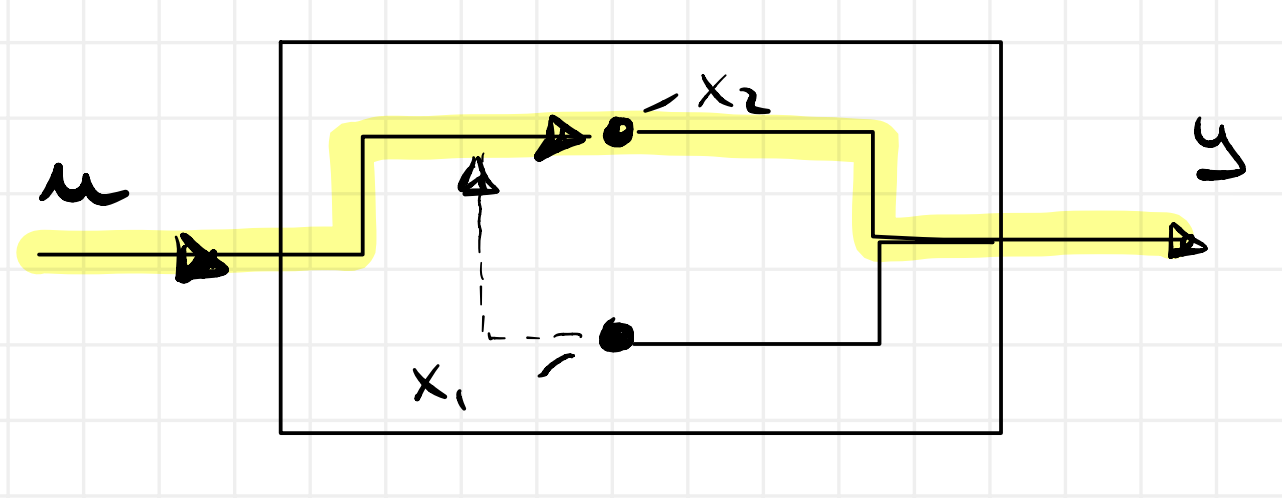
\includegraphics[width=4cm]{sist-nonragg}
			\end{center}
			In questo caso si può affermare che il sistema non è completamente raggiungibile dall'ingresso $u$: gli autovalori della matrice di stato sono in quantità superiore dei poli dell'uscita che risponde all'impulso e dunque l'analisi di stabilità esterna può non coincidere con la stabilità esterna.
			
		\end{esempio}
	
	\subsection{Osservabilità di un sistema dinamico}
		Si consideri il sistema dinamico mostrato in figura \ref{sist-inoss} composto da due masse che possono scorrere sul piano. L'attuatore idraulico (o il sensore di elongazione) permettono dunque di determinare uno spostamento (o misurarlo rispettivamente) relativo tra le due masse $m_1,m_2$, ma non permettono di determinare la posizione assoluta delle stesse.	
	
		\figura{5}{3}{sist-inoss}{sistema composto da due carrelli in cui $m_1$ è collegato a telaio da una molla, mentre $m_2$ è collegato ad $m_1$ tramite una molla e un attuatore/sensore (evidenziato in giallo).}{sist-inoss}
		
		Questo è un esempio pratico di \textbf{sistema non completamente raggiungibile/osservabile}: analizzando la rappresentazione in forma di stato del sistema dinamico ci si accorge infatti che l'ordine del denominatore $D(s)$ è minore dell'ordine del sistema dinamico di partenza, il che implica che nel processo di analisi dell'impulso è stata commessa una cancellazione.
		
		\vspace{3mm}
		
		La sola ispezione delle equazioni di stato non sempre permette di individuare se il sistema è completamente raggiungibile o osservabile; per effettuare tale analisi è necessario ricorrere a strumenti quali:
		\begin{itemize}
			\item il confronto dell'ordine del polinomio a denominatore $D(s)$ con l'ordine del sistema (se il primo ha grado inferiore del secondo, allora sono state effettuate delle cancellazioni critiche);
			\item utilizzare dei test specifici di raggiungibilità ed osservabilità; tali metodi (che non verranno trattati) si basano sulla formulazione della matrice di raggiungibilità $R = f(A,B)$ e dalla matrice di osservabilità $O = f(A,C)$.
		\end{itemize}
		
		
	\subsection{Osservazioni e BIBO stabilità}
		Dato un sistema dinamico lineare tempo invariante, e ipotizzando che lo stesso sia completamente raggiungibile/osservabile, allora la stabilità del sistema stesso è una proprietà strutturale, ossia è indipendente dalla rappresentazione che si fa dello stesso (una scelta di diverse variabili di stato deve necessariamente portare alla stessa conclusione sui risultati).
		
		Per questo tipo di sistemi l'asintotica stabilità in uscita dipende solamente dall'ingresso $u(t)$, e non dalle specifiche condizioni iniziali $x_0$ del sistema: tale asserzione è particolarmente desiderata nelle applicazioni reali in quanto si \textit{eliminano} così gli effetti di disturbo (il movimento di equilibrio dipende solo dall'ingresso, e non dallo stato).
		
		Sistemi lineari tempo invarianti asintoticamente stabili sono caratterizzati dall'avere uno e un solo punto di equilibrio (unico): gli autovalori della matrice di stato sono tutti a parte reale negativa. Essendo garantita la possibilità di calcolare l'inversa (per il fatto che $\det A \neq 0$), allora si può determinare l'equilibrio del sistema ed essendo per ingressi costanti l'uscita asintotica, allora l'uscita tende al movimento di equilibrio.
		
		\begin{concetto}
			Un sistema è dunque detto \textbf{BIBO stabile} se e solo se ad ogni suo ingresso limitato (\textit{Bounded Input}) corrisponde un'uscita limitata (\textit{Bounded Output}).
		\end{concetto}
		A questo punto è possibile dimostrare che condizione necessaria e sufficiente affinché un sistema lineare tempo invariante sia BIBO stabile è che i poli dell'uscita ottenuta da uno scalino in ingresso abbia poli siano tutti a parte reale positiva (ossia che il sistema sia esternamente asintoticamente stabile).
		
	\subsection{Stabilità per sistemi non lineari}
		In generale il concetto di \textit{stabilità} di un sistema dinamico è associato al \textit{movimento dell'uscita} e non al \textit{sistema} stesso (per sistemi lineari spesso tale concetto può essere confuso in quanto la stabilità è una proprietà del sistema, ma non vale in generale per sistemi non lineari). A questo punto per analizzare il tipo di stabilità dei movimenti dell'uscita di sistemi non lineari è possibile utilizzare diversi strumenti matematici; verranno qui accennati due metodi per lo studio del movimento di equilibrio di un sistema per questo tipo di sistemi.
		
		\paragraph{Metodo indiretto di Lyapunov} Il \textbf{metodo indiretto di Lyupanov} si basa sullo studio della stabilità del movimento dell'uscita del sistema linearizzando lo stesso nell'intorno del punto di equilibrio. Facendo così è possibile trasformare il sistema non lineare in un sistema lineare che può essere analizzato con le metodologie accennate in precedenza.
		
		Se analizzando il sistema linearizzato si conclude che lo stesso è semplicemente stabile, allora non è possibile asserire alcuna conclusione sulla stabilità del sistema non lineare originario (potrebbe infatti essere che, nella realtà, il sistema sia asintoticamente stabile oppure instabile).
		
		\paragraph{Metodo grafico per sistemi scalari} Per sistemi non lineari scalari, ossia di ordine $n=1$, è possibile analizzarne la stabilità tramite un metodo grafico. Facendo riferimento per esempio all'equazione di stato $\dot x = f(x,\overline u)$ in figura \ref{graf-scal} associata all'ingresso costante $\overline u$, è possibile osservare che i punti di equilibrio sono quelli che annullano la derivata $\dot x$ (indicati con $\overline x_1,\overline x_2,\overline x_3$).		
			
		\figura{6}{1}{graf-scal}{grafico di riferimento per l'analisi grafica di stabilità di un sistema non lineare.}{graf-scal}
		
		Per studiare la stabilità dei punti di equilibrio determinati è possibile pensare di perturbare lo stato $x$ nell'intorno di uno dei punti di equilibrio $\overline x_i$. Osservando il verso della derivata $\dot x$ è infatti possibile predire lo spostamento dello stato: per esempio nel caso di derivata positiva (indicata dalle frecce gialle nel diagramma di riferimento) la variabile di stato perturbata tenderà ad andare verso destra, mentre se la derivata è negativa (in blu) lo stato tenderà a spostarsi verso sinistra.
		
		A questo punto è possibile osservare che il punto di equilibrio $\overline x_1$ è asintoticamente stabile in quanto una perturbazione (non troppo accentuata) dello stato verrà \textit{riportata} per l'effetto della derivata al punto di equilibrio. Al contrario perturbando i punti $\overline x_2,\overline x_3$ lo stato, per effetto della derivata, tenderà a divergere dal punto di equilibrio: il sistema è dunque instabile.
		
		\begin{esempio}{: stabilità di un sistema non lineare scalare}
			Si consideri il sistema dinamico non lineare di ordine unitario la cui rappresentazione di stato è
			\[ \begin{cases}
				\dot x = - x^3 + u \\ y = x
			\end{cases} \]
			Volendo studiare la stabilità per un ingresso costante $\overline u = 0$, risolvendo l'equazione di stato si ottengono 3 soluzioni coincidenti per lo stato di equilibrio del sistema $\overline x_{1,2,3} = 0$. Volendo provare a determinare il tipo di stabilità del sistema lineare è possibile pensare di \textbf{linearizzare} la rappresentazione di stato del sistema, ossia determinando le matrici $A,B,C,D$ come visto a pagina \pageref{sec:intro:linearizzazione}; in particolare essendo il sistema scalare ogni matrice sarà di dimensione $1\times 1$, ossia un coefficiente numerico:
			\[ A = \left. \pd f x\right|_{\overline x,\overline u} = - 3x^2 \Big|_{\substack{x = 0 \\ u = 0}} = 0 \qquad
			B = \left. \pd f u\right|_{\overline x,\overline u} = 1 \Big|_{\substack{x = 0 \\ u = 0}} = 1 \]
			\[ C = \left. \pd g x\right|_{\overline x,\overline u} = 1 \Big|_{\substack{x = 0 \\ u = 0}} = 1 \qquad 
			D = \left. \pd g u\right|_{\overline x,\overline u} = 0 \Big|_{\substack{x = 0 \\ u = 0}} = 0 \]
			
			Per procedere con lo studio della stabilità del sistema è necessario determinare la risposta allo scalino del sistema che è determinata dall'equazione
			\[ C\big(sI-A\big)^{-1} B +  D = \frac 1 s \]
			A questo punto l'unico polo dell'uscita $Y(s)$ è posto nella posizione $s=0$, e dunque se il sistema fosse lineare significherebbe che il sistema è \textbf{semplicemente stabile}. Tuttavia essendo il sistema non lineare, allora non è possibile affermare con precisione il tipo di stabilità. 
			\begin{multicols}{2}
			Analizzando \textbf{graficamente} invece l'equazione di stato risulta evidente immediatamente che nella realtà il sistema è \textbf{asintoticamente stabile}: spostando infatti lo stato dalla sua condizione di equilibrio $\overline x=0$, il \textit{segno} della derivata tenderà sempre a riportarlo verso il punto di equilibrio (che è per questo asintoticamente stabile).
			
			\begin{center}
				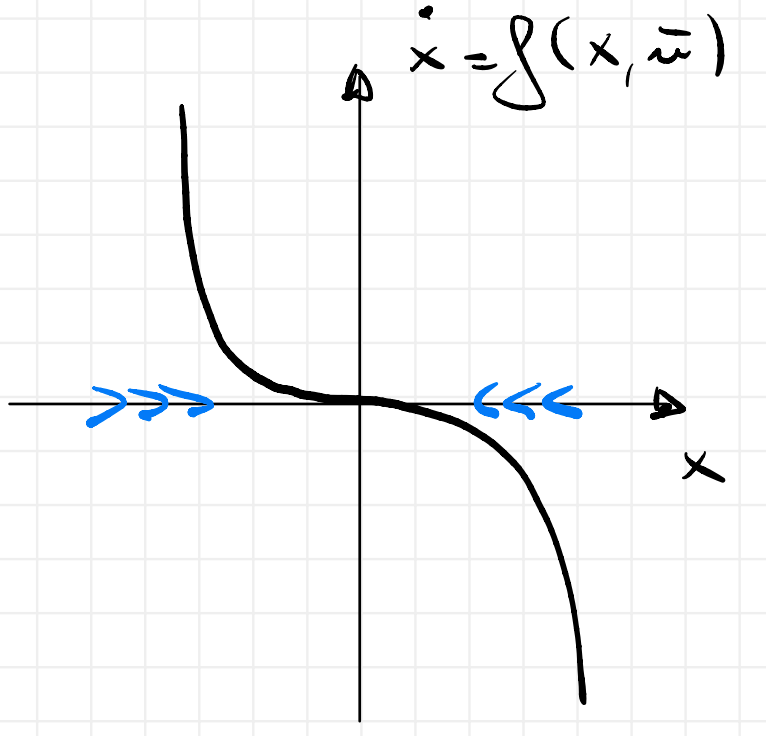
\includegraphics[width=3cm]{graf-scal-es}
			\end{center}
		\end{multicols}
		
		\end{esempio}
		
\section{Funzione di trasferimento}
	In precedenza si er descritto il movimento d'uscita di un sistema dinamico lineare nel dominio di Laplace, osservando che (come nel dominio del tempo) esso prevedeva sia una componente di movimento libero che di movimento forzato (eq. \ref{eq:lti:movimenti}, pag. \pageref{eq:lti:movimenti}).
	\begin{concetto} Considerando ora solamente la parte di movimento forzato, ossia imponendo che lo stato iniziale $x_0$ sia nullo, è possibile determinare la cosiddetta \textbf{funzione di trasferimento} $G(s)$ di un sistema dinamico tempo invariante
		\begin{equation}
			Y(s) = \underbrace{\Big(C\big(sI-A\big)^{-1}B+D\Big)}_{G(s)} U(s)
		\end{equation}
	\end{concetto}
	La funzione di trasferimento dunque permette di correlare direttamente l'uscita $Y$ di un sistema (nel dominio di Laplace) con la sua uscita; considerando il movimento forzato espresso nel dominio del tempo come
	\[ y(t) = C\int_0^t e^{A(t-\tau)}Bu(\tau)\, d\tau + Du(t) \]
	appare evidente che la relazione ingresso-uscita mediante funzione di trasferimento è molto più \textit{facile} da calcolare rispetto alla rispettiva relazione nel dominio del tempo.
	
	Nella pratica è possibile determinare la funzione di trasferimento di un sistema lineare attraverso due metodologie:
	\begin{itemize}
		\item supponendo di conoscere il modello analitico del sistema, ossia note le matrici $A,B,C,D$ che lo descrivono, è possibile determinare \textit{a priori} analiticamente la funzione di trasferimento applicando la definizione:
		\[ G(s) = C\big(sI-A\big)^{-1}B+D \]
		\item se non si conosce il modello del sistema ma è tuttavia possibile calcolare le trasformate di un ingresso arbitrario e la rispettiva uscita, si può determinare la funzione di trasferimento per inversione del modello:
		\[ G(s) = \frac{Y(s)}{U(s)}\]
	\end{itemize}
	

	\begin{concetto}
		La \textbf{funzione di trasferimento} rappresenta di fatto la \textbf{risposta all'impulso} di un sistema dinamico: considerato infatti che $\trasf{\imp(t)} = 1 $ per ogni valore $s$, allora calcolando l'uscita del sistema si osserva che essa coincide con la funzione di trasferimento:
		\[ Y(s) = G(s) \cancel 1 \qquad \textrm{se } U(s) = \trasf{\imp(t)} \]
	\end{concetto}	

	Nel caso particolare di sistema lineare SISO la funzione di trasferimento è di fatto una trasformata razionale (rapporto di due polinomi), mentre se il sistema è MIMO $G(s)$ rappresenta di fatto una \textbf{matrice di trasferimento}, ossia una \textit{collezione} di trasformate razionali caratterizzate dall'avere il polinomio a denominatore comune; in questo caso l'elemento $g_{ij} \in G(s)$ rappresenta la funzione di trasferimento sussistente tra l'$i$-esima uscita e il $j$-esimo ingresso (vigendo il principio di sovrapposizione degli effetti, l'uscita complessiva del sistema sarà determinata dalla somma dei contributi di tutti gli ingressi).
	
	\vspace{3mm} E' anche possibile osservare che l'analisi di stabilità esterna fin'ora analizzata di fatto si basava sul determinare la posizione dei poli nel piano complesso della funzione di trasferimento $G(s)$ del sistema dinamico; per come già visto nel caso di sistemi lineari tempo invarianti completamente raggiungibili/osservabili tali poli coincidono con gli autovalori della matrice di stato $A$ e la funzione di trasferimento è una proprietà \textit{strutturale} del sistema, ossia indipendente dalla scelta delle variabili di stato per descrivere il problema.
	
	\subsection{Parametrizzazioni della funzione di trasferimento}
		La stessa funzione di trasferimento $G(s)$ può essere espressa in diverse formulazioni alternative. Essa infatti (ai fini di questo corso) è sempre descritta come il rapporto tra due polinomi $N(s)$ e $D(s)$: tali polinomi possono infatti essere descritti, in maniera equivalente, tramite una \textit{forma fattorizzata} e una \textit{forma polinomiale} come nell'esempio che segue
		\[ \underbrace{(s+1)(s+2)}_\textrm{fattorizzata} = \underbrace{s^2+3s + 2}_\textrm{polinomiale} \]
	
		\begin{concetto}
			Sfruttando l'idea di \textit{riscrivere} in maniera alternativa i polinomi, in equazione \ref{eq:lti:parametrizzazione} è possibile osservare 3 rappresentazioni analoghe una funzione di trasferimento, in particolare sono rappresentante la \textbf{forma polinomiale} (a), la \textbf{forma fattorizzata di Nyquist} (b) e \textbf{forma fattorizzata di Bode} (c).
			\begin{subequations} \label{eq:lti:parametrizzazione}
			\begin{align}
				G(s) & = \frac{\beta_ns^n + \beta_{n-1}s^{n-1} + \dots + \beta_1 s + \beta_0}{s_n + \alpha_{n-1}s^{n-1}+ \dots + \alpha_0} \\
				& = \frac{\rho}{s^g} \frac{ \prod_i \big(s + z_i\big) \prod_i \big( s^2 + 2\eta_i\alpha_i s+ \alpha_i^2 \big) }{ \prod_i \big(s + p_i\big) \prod_i \big( s^2 + 2\xi_i\omega_i s+ \omega_i^2 \big) } \\
				& = \frac{\mu}{s^g} \frac{ \prod_i \big(\tau_is + 1\big) \prod_i \left( \frac{s^2}{\alpha_i^2} + 2 \frac{\eta_i}{\alpha_i} s + 1  \right) } { \prod_i \big(T_is + 1\big) \prod_i \left( \frac{s^2}{\omega_i^2} + 2 \frac{\xi_i}{\omega_i} s + 1  \right) }
			\end{align}
			\end{subequations}
		\end{concetto}
	
		La forma polinomiale (\ref{eq:lti:parametrizzazione}a) di fatto è caratterizzata da $2n-1$ coefficienti associati ai parametri $\alpha_i,\beta_i$ dei termini del polinomio. Questa forma risulta essere di poca utilità pratica in quanto è difficile determinare la stabilità del sistema dinamico in quanto non è immediato determinare i poli della funzione di trasferimento: per questo motivo sono più \textit{comode} le forme fattorizzate di Nyquist e di Bode.
		
		In entrambe le forme fattorizzate è possibile osservare la presenza del parametro $g$: esso prende il nome di \textbf{grado} del sistema dinamico e rappresenta il numero di poli (se positivo) o zeri (se negativo) presenti nell'origine. \\
		Per quanto riguarda la forma fattorizzata di Nyquist (\ref{eq:lti:parametrizzazione}b) si indica con  $\rho$ la \textbf{costante di trasferimento}, con $z_i\neq 0$ i valori opposti degli zeri reali della funzione di trasferimento, mentre $p_i \neq 0$ rappresentano l'opposto dei poli reali (termini associati alla produttoria \textit{a sinistra} di numeratore e denominatore). Le produttorie \textit{a destra} di numeratore/denominatore determinate dai coefficienti $\eta_i/\xi_i$ e $\alpha_i/\omega_i$ sono utilizzate per rappresentare invece i poli complessi coniugati. In particolare i termini $\eta_i,\xi_i$ (il cui modulo è sempre inferiore o pari a 1) rappresentano gli \textbf{smorzamenti del polo}, mentre i termini $\alpha_i,\omega_i > 0$ rappresentano le \textbf{pulsazioni naturali}.\\
		La forma fattorizzata di Bode (\ref{eq:lti:parametrizzazione}c) è molto simile a quella di Nyquist, in quanto si può pensare come la sua \textit{ normalizzazione}; il termine $\mu$ prende il nome di \textbf{guadagno} mentre i termini $\tau_i = 1 / z_i$ e $T_i = 1 / p_i$ rappresentano le \textbf{costanti di tempo} di zeri e poli rispettivamente.
		
		Nota la costante di trasferimento $\rho$ nella forma di Nyquist di può ricavare il guadagno nella forma di Bode tramite la relazione
		\[ \mu = \rho \frac{\prod_i z_i \prod\alpha_i^2}{\prod_i p_i \prod\omega_i^2} \] 
		
		\paragraph{Poli (e zeri) complessi coniugati} Si consideri un polo di smorzamento $\xi$ e pulsazione naturale $\omega$ (ma il ragionamento è analogo per gli zeri di una funzione di trasferimento), allora la rappresentazione nella forma di Nyquist e Bode vale rispettivamente
		\[ \underbrace{s^2 + 2 \xi \omega s + \omega^2}_\textrm{Nyquist} \qquad \leftrightarrow \qquad \underbrace{\frac{s^2}{\omega^2} +2 \frac \xi \omega s + 1 }_\textrm{Bode} \]
		 In entrambi i casi calcolando le radici di tali espressioni si ottengono i valori
		 \[ s_{1,2} = \underbrace{- \xi \omega}_\textrm{Re} \pm i\underbrace{ \omega \sqrt{1 - \xi^2}}_\textrm{Im} \]
		 Le due radici sono infatti dei numeri complessi composti da una parte reale pari a $-\xi\omega$ e da una parte immaginaria di valore $\omega \sqrt{1-\xi^2}$. Volendo dare un \textit{significato rappresentativo} (come in figura \ref{complessi}) alle due grandezze, i poli complessi coniugati possono essere descritti nel piano dei numeri immaginari come dei punti (descritti da vettori) distanti $\omega$ dal centro del piano e con angolo $\theta$ (calcolato come in figura \ref{complessi}) tale che
		 \[ \xi = \cos\theta \]
		 
		\figura{6}{1}{complessi}{rappresentazione nel piano dei numeri immaginari di un polo complesso coniugato.}{complessi}
		Essendo i poli complessi coniugati, determinato un polo l'altro può essere ottenuto specchiando il primo rispetto all'asse dei numeri reali. Poli con smorzamento positivo sono posizionati nel semipiano a parte reale negativa, mentre smorzamenti negativi sono nel semipiano destro a parte reale positiva.
		 
	\subsection{Sistemi a ritardo di tempo}
		\begin{concetto}
			Sono detti \textbf{sistemi a ritardo di tempo} tutti quei sistemi che \textit{ritardano} l'uscita; in particolare l'uscita $y(t)$ è pari all'ingresso $u$ in ritardo di un coefficiente $\tau$, ossia $y(t) = u(t-\tau)$. Sfruttando la proprietà di traslazione nel dominio del tempo (eq. \ref{eq:class:proptraslazionetempo}, pag. \pageref{eq:class:proptraslazionetempo}) la funzione di trasferimento di questo sistema può dunque essere espressa come
			\begin{equation}
				G(s) = e^{-\tau s}
			\end{equation}
		\end{concetto}
		Questo tipo di sistema dinamico sarà l'unico \textit{non canonico} nel corso: la sua trasformata infatti non è razionale ma è una funzione trascendente (cosa che in generale può dare problemi nell'analizzare il problema).	
	
\section{Studio del legame ingresso-uscita}
	Avendo determinato la funzione di trasferimento $G(s)$ di un sistema dinamico tempo invariante tramite la forma fattorizzata di Nyquist/Bode (eq. \ref{eq:lti:parametrizzazione}), si vuole ora cercare di interpretare il \textit{significato} dei vari elementi che compongono le parametrizzazioni (poli, zeri, smorzamenti, pulsazioni...) e come gli stessi influenzano i sistemi dinamici. Particolarmente importante sarà dunque analizzare due tipi di risposta: quella ad un ingresso a scalino (per determinare le proprietà di transitorio del sistema) e quelle di un ingresso sinusoidale.
	
	\subsection{Risposta allo scalino}
		La risposta allo scalino di un sistema dinamico è interessante da analizzare in quanto permette di studiare il comportamento di un sistema che passa da una condizione di quiete ad un'altra condizione di quiete diversa (chiaramente affinché ciò si verifichi si deve garantire l'asintotica stabilità del sistema che si sta analizzando). In particolare essendo il sistema lineare è sufficiente calcolare la risposta del sistema allo scalino unitario in quanto ogni altro tipo di scalino può essere determinato tramite il principio di sovrapposizione degli effetti.
		
		\begin{concetto}
			La \textbf{risposta allo scalino} viene utilizzata per determinare molte delle proprietà \textit{salienti} del transitorio di un sistema dinamico, in particolare:
			\begin{itemize}
				\item il \textbf{valore iniziale} $y_0$ (ed eventualmente le sue derivate $\dot y_0,\ddot y_0,\dots$) dell'uscita del sistema;
				\item il \textbf{valore asintotico} $y_\infty$ dell'uscita, ossia il valore cui tende la stessa per $t\rightarrow \infty$;
				\item il \textbf{tempo di assestamento} $t_a$, ossia dopo quanto tempo la risposta del segnale può essere approssimata al valore asintotico, e l'eventuale \textbf{periodo} $T$ di oscillazioni del sistema;
				\item l'eventuale \textbf{sovra-elongazione} (\textit{overshoot}) $s_\%$ dell'uscita, definita come il rapporto percentuale tra uscita massima $y_{max}$ nella fase transitoria e valore asintotico:
				\[ s_\% = \frac{|y_{max} - y_\infty|}{y_\infty} 100 \]
			\end{itemize}
		\end{concetto}
		Nel seguito verranno dunque discusse alcune casistiche di funzioni di trasferimento \textit{semplici} ma i cui risultati verranno estesi a carattere più generale
		
		\subsubsection{Sistemi del primo ordine con un polo nell'origine}
			Si consideri il sistema di ordine unitario la cui parametrizzazione della funzione di trasferimento è $G(s) = \dfrac \mu s$, dove $\mu$ è il guadagno del sistema; questo sistema presenta dunque un solo polo nell'origine (mentre non sono presenti zeri). A questo punto per studiare la risposta allo scalino è necessario moltiplicare $G(s)$ per la trasformata dell'ingresso dello scalino, ossia
			\[ Y(s) = G(s) U(s) = \frac \mu s \frac 1 s = \frac{\mu}{s^2} \]
			
			Essendo verificate le condizioni iniziali del teorema \ref{teor:valiniziale} del valore iniziale (pag. \pageref{teor:valiniziale}) è possibile calcolare l'uscita $y_0$ nel dominio del tempo tramite la relazione
			\[ y_0 = \lim_{s\rightarrow\infty}s \, Y(s) = \lim_{s\rightarrow\infty}\cancel{s}  \frac{\mu}{s^{\cancel{2}}} = 0 \]
			Osservato che l'uscita iniziale è nulla è possibile pensare di calcolarne la derivata: sfruttando la relativa proprietà (eq. \ref{eq:class:derivata}, pag. \pageref{eq:class:derivata}) è possibile affermare infatti che $\trasf{\dot y} = s Y(s) - y(0)$. Noto che $y(0)=y_0=0$ (ed essendo ancora la trasformata razionale) è possibile applicare ulteriormente il limite del valore iniziale e dunque
			\[ \dot y_0 = \lim_{s\rightarrow \infty} s \big(sY(s) - y_0\big) = \lim_{s\rightarrow\infty} \cancel{s^2} \frac{\mu}{\cancel{s^2}} = \mu \]
	
			Per quanto riguarda la risposta asintotica è possibile invece utilizzare il teorema \ref{teor:valfinale} del valore finale (pag. \pageref{teor:valfinale}): essendo la trasformata razionale e con poli a parte reale nulla allora vale che
			\[ y_\infty = \lim_{s\rightarrow 0} s\,Y(s) = \lim_{s\rightarrow 0} \frac \mu s = \infty \]
			
			Questi risultati in realtà sono \textit{attendibili} rispetto a quello che ci si aspettava dal sistema: anti-trasformando l'uscita $Y(s)$ si osserva infatti che
			\[ y(t) = \anti{F(s)} = \mu \anti{\frac 1 {s^2}} = \mu \ramp(t) \]
			Osservando infatti il grafico dell'uscita $y(t)$ nel dominio del tempo (fig. \ref{scal1-a}) si osserva che l'uscita parte da valore nullo e con una pendenza pari a $\mu$ diverge a $\infty$. Essendo il sistema non asintoticamente stabile (il polo in $s=0$ afferma che il sistema è semplicemente stabile) allora esso non potrà essere neanche BIBO stabile: ad un ingresso limitato quale lo scalino è associata infatti un'uscita non limitata.
			
			\figura{5}{1}{scal1-a}{risposta allo scalino di un sistema con funzione di trasferimento $G(s) = \mu / s$ con $\mu = 10$.}{scal1-a}
	
			\begin{concetto}
				Facendo riferimento all'esempio appena mostrato è possibile affermare che, a carattere generale, se il tipo $g$ della funzione è positivo non nullo (in questo caso essendo presente un polo nell'origine si ha $g=1$) allora la risposta allo scalino del sistema non si assesta a nessun valore di regime.
			\end{concetto}
	
		\subsubsection{Sistema del primo ordine con polo non nell'origine}
			Si consideri ora un sistema di ordine $n=1$ con un polo a parte reale negativa non nulla (in modo da garantire l'asintotica stabilità del sistema) la cui funzione di trasferimento fattorizzata in forma di Bode vale
			\[ G(s) = \mu \frac 1{Ts + 1} \qquad \xrightarrow[\textrm{scalino}]{\textrm{risposta allo}} \quad Y(s) = G(s) U(s) =  \frac \mu {s\big(Ts + 1\big)} \]
			
			Calcolata dunque la trasformata $Y(s)$ della risposta allo scalino applicando il teorema del valore iniziale è possibile calcolare che $y_0=0$, mentre $\dot y_0 = \mu / T$ (come nel caso di polo nell'origine il valore iniziale è nullo, tuttavia la derivata dell'uscita risulta divisa per la costante di tempo $T$ del polo). Applicando invece il teorema del valore finale si osserva che
			\[ y_\infty = \lim_{s\rightarrow 0} s\,Y(s) = \lim_{s\rightarrow 0} \frac \mu{s\big(Ts + 1\big)} = \mu \]
			\begin{nota}
				E' possibile applicare il teorema del valore finale solamente perché si era ipotizzato inizialmente che il polo fosse a parte reale negativa (ossia deve essere che $T>0$), altrimenti non sarebbero rispettate le ipotesi di applicabilità.
			\end{nota}
			Effettuando l'anti-trasformazione con il metodo di Heaviside è possibile risalire all'uscita $y(t)$  del sistema nel dominio del tempo, e in particolare
			\[ y(t) = \anti{\frac \mu{s\big(Ts + 1\big)}} = \mu \left(1 - e^{-t/T}\right)\]
			Osservando la rappresentazione grafica dell'uscita (figura \ref{scal1-b}) è possibile osservare che $y(t)$ non presenta oscillazioni (e dunque il relativo periodo è pari a zero) e come anche l'elongazione percentuale $s_\%$ sia nulla.
			\figura{5}{1}{scal1-b}{risposta allo scalino di un sistema con funzione di trasferimento $G(s) = \frac \mu {Ts + 1}$ con parametri $\mu = 10$ e $T=2$.}{scal1-b}
			
			A questo punto non resta altro che calcolare il tempo di assestamento $t_a$ del sistema, ossia quel valore che, scelta una tolleranza $\varepsilon$, verifica la relazione
			\begin{equation} \label{eq:lti:tolleranza}
				\big|y(t_a) - y_\infty\big| \leq \varepsilon \, y_\infty
			\end{equation}
			
			\begin{concetto}
				Impostata una tolleranza $\varepsilon = 0.01$ (ossia $1\%$) tramite calcolo esplicito della relazione \ref{eq:lti:tolleranza} è possibile determinare che il \textbf{tempo di assestamento} di una funzione di trasferimento ad un solo polo che vale
				\begin{equation} \label{eq:lti:tempo1polo}
					t_a = 4.6T \approx 5T
				\end{equation}
			\end{concetto}
			Questo significa che ad un tempo $t$ pari a 5 volte la costante di tempo $T$ del polo l'errore che si commette a considerare l'uscita asintotica rispetto a quella reale è inferiore all'$1\%$ e dunque, a livello ingegneristico, è possibile considerare che il sistema è a regime.
			\begin{osservazione}
				Il tempo di assestamento non dipende dal guadagno $\mu$ del sistema, ma solamente dalla costante di tempo $T$ del polo.
				\begin{center}
					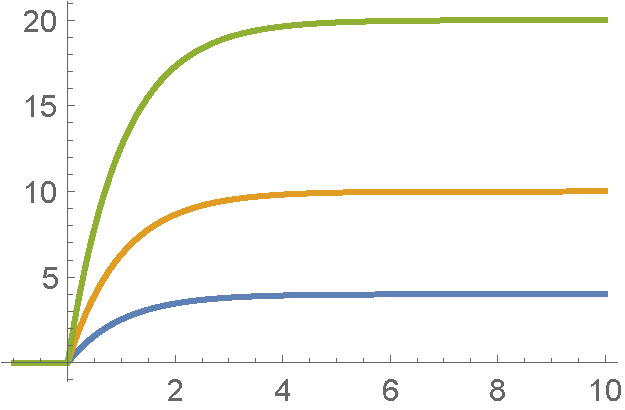
\includegraphics[width=5cm]{scal1-c}
				\end{center}
				In figura sono infatti riportate 3 funzioni di trasferimento per le quali la costante di tempo è uguale e pari a $T=1$, mentre il guadagno è variabile ($\mu = 3,10,20$): è possibile osservare che in tutti i casi dopo il tempo $t_a = 5T=5$ la risposta può essere considerata pressoché stazionaria.
			\end{osservazione}
			
			Rappresentando nel piano dei numeri immaginari i poli si osserva che la loro posizione nell'asse dei numeri reali dipende dalla costante di tempo $T$ e vale $-1/T$ (figura \ref{lentoveloce}): questo significa che dati due sistemi per cui $T_1 > T_2$ allora il primo sistema sarà più lento (per via del maggiore tempo di assestamento) e dunque il polo associato sarà più vicino all'origine. 
			
			\figura{5}{1}{lentoveloce}{posizione nel piano complesso di due poli con costanti di tempo $T_1>T_2$.}{lentoveloce}
			
			Questo significa che per avere dei sistemi dinamici con tempo di assestamento molto basso è necessario \textit{spostare} i poli il più possibile lontano (\textit{verso sinistra}) dal centro del piano dei numeri complessi, diminuendo il più possibile la parte reale, il che può essere fatto diminuendo il più possibile la costante di tempo (in figura \ref{scal1-d} è mostrato un esempio).
		
			\figura{5}{1}{scal1-d}{risposta allo scalino di un sistema con funzione di trasferimento $G(s) = \frac \mu {Ts + 1}$ con guadagno $\mu = 10$ e costanti di tempo $T=1$ (funzione arancione) e $T = 3$ (blu).}{scal1-d}
		\subsubsection{Sistema del secondo ordine a poli coincidenti}
			Si consideri ora un sistema del secondo ordine a poli coincidenti (a costante di tempo $T >0$ in modo da garantire che i poli siano a parte reale negativa) la cui funzione di trasferimento e relativa risposta allo scalino sono descritte dalle trasformate razionali
			\[ G(s) =  \frac \mu{\big(Ts + 1\big)^2} \qquad \xrightarrow[\textrm{scalino}]{\textrm{risposta allo}} \quad Y(s) = G(s) U(s) = \frac \mu{s\big(Ts + 1\big)^2} \]
			
			Applicando il teorema del valore iniziale si calcola che sia $y_0$ che la sua derivata $\dot y_0$ sono nulle, mentre il primo termine non nullo è la derivata seconda dell'uscita che risulta valere $\ddot y_0 = \mu / T^2$.
			\begin{osservazione}
				A livello intuitivo è dunque possibile iniziare a pensare che il numero di poli della funzione di trasferimento è associato all'ordine del primo valore di derivata che risulterà non essere nulla al tempo iniziale.
			\end{osservazione}
			Avendo ipotizzato che il polo multiplo della funzione di trasferimento sia a parte reale negativa è dunque possibile applicare il teorema del valore finale e osservare che l'uscita asintotica (come nel caso di un solo polo a parte reale negativa) vale $y_\infty = \mu$. \\			
			A questo punto è possibile anti-trasformare l'uscita $Y(s)$ tramite il metodo di Heaviside che determina l'uscita
			\[ y(t) = \anti{ \frac \mu{s(Ts + 1)^2}} = \mu \left( 1- e^{-t/T} - \frac t T e^{-t/\tau} \right) \] 
			\begin{nota}
				La trasformata razionale dell'uscita $Y(s)$ è di ordine 3 e la scomposizione di Heaviside associata a tale funzione vale
				\[ Y(s) = \frac As + \frac B{Ts+1} + \frac C{\big(Ts+1\big)^2} \]
				Determinando dunque i coefficienti $A$ (che risulterà valere $\mu$), $B$ ($-\mu$) e $C$ ($-\mu/T$) l'anti-trasformata è composta da $y(t) = A \scal(t) + Be^{-t/T} + Ct e^{-t/T}$.					 
			\end{nota}
			
			\figura{5}{1}{scal2-a}{risposta allo scalino di un sistema con funzione di trasferimento $G(s) = \frac \mu {(Ts + 1)^2}$ con parametri $\mu = 10$ e $T=2$.}{scal2-a}
			
			Graficando l'uscita del sistema dinamico (figura \ref{scal2-a}) si osserva che la funzione non è periodica ($y$ è composta da un solo esponenziale) e non si ha neanche sovra-elongazione (in quanto $y_{max} = y_\infty$). Invertendo l'equazione \ref{eq:lti:tolleranza} per l'uscita nel dominio del tempo appena determinata, considerando una tolleranza $\varepsilon = 1\%$ allora si dimostra che il tempo di assestamento del sistema vale
			\begin{equation}\label{eq:lti:tempo2poli}
				t_a = 6.64T
			\end{equation}
			
			Confrontando questo risultato con quello ottenuto per i sistemi ad un polo (eq. \ref{eq:lti:tempo1polo}) è possibile osservare che, a parità di costante di tempo $T$, i sistemi a polo multiplo sono più lenti (figura \ref{scal2-b}).
			\figura{5}{1}{scal2-b}{risposta allo scalino di un sistema ad un polo (arancione) e due poli coincidenti (azzurro) con costanti di tempo e guadagno eguali.}{scal2-b}
		
		\subsubsection{Sistema a due poli reali distinti}
			Considerando ora un sistema a due poli reali distinti (a costanti di tempo $T_1,T_2>0$ in modo da garantire l'asintotica stabilità del sistema) allora è possibile esprimere la sua funzione di trasferimento e relativa risposta allo scalino tramite le trasformate razionali
			\[ G(s) =  \frac \mu{\big(T_1s + 1\big) \big(T_2s + 1\big) } \qquad \xrightarrow[\textrm{scalino}]{\textrm{risposta allo}} \quad Y(s) = G(s) U(s) = \frac \mu{s\big(T_1s + 1\big) \big(T_2s + 1\big) } \]
			Tramite i teoremi di valore iniziale e finale si osserva che, come nel caso precedente, $y_0 = \dot y_0 = 0$ e la risposta asintotica $y_\infty$ è costante e pari al guadagno $\mu$; l'unica variazione che si può osservare è nel calcolo della derivata seconda del valore iniziale che risulta valere $\ddot y_0 = \dfrac \mu {T_1T_2}$. \\
			A questo punto anti-trasformando con il metodo di Heaviside l'uscita $Y(s)$ del sistema può essere espressa nel dominio del tempo arrivando alla conclusione che
			\[ y(t) = \mu \Big(  1 - \underbrace{\frac{T_1}{T_1-T_2} e^{-t/T_1}}_{\substack{\textrm{esponenziale} \\ \textrm{associato} \\ \textrm{a $T_1$}}} + \underbrace{\frac{T_2}{T_1-T_2} e^{-t/T_2} }_{\substack{\textrm{esponenziale} \\ \textrm{associato} \\ \textrm{a $T_2$}}} \Big) \]
			Il risultato dell'uscita può essere rappresentata nel dominio del tempo tramite il grafico in figura \ref{scal2-c}. Si osserva che essendo la risposta esponenziale allora non si ha periodicità nel segnale e anche la sovra-elongazione $s_\%$ è nulla. Per quanto riguarda il tempo di assestamento è possibile osservare che, considerando per esempio $T_1>T_2$, il tempo di assestamento del sistema dovrà sempre essere compresa tra il valore minimo associato ad una funzione di trasferimento con polo singolo di costante $T_1$ e il valore massimo rappresentato da un sistema a polo doppio con medesima costante di tempo.
						
			\figura{5}{2}{scal2-c}{risposta allo scalino di un sistema con funzione di trasferimento $G(s) = \frac \mu {(T_1s + 1)(T_2s+1)}$ con parametri $\mu = 10$, $T_1=3$ e $T_2 = 1.5$ (in azzurro); in arancione è rappresentata la zona rispetto al quale il comportamento del sistema a due poli distinti può appartenere.}{scal2-c}
			
			Nel caso limite in cui $T_2 = T_1$ infatti il comportamento del sistema coincide con quello di una funzione di trasferimento a due poli reali coincidenti e per cui il tempo di assestamento vale $t_a = 6.64 T$ (eq. \ref{eq:lti:tempo2poli}). Al contrario nel caso in cui $T_2 \ll T_1$ l'esponenziale associato a $T_2$ si \textit{esaurisce} molto rapidamente (raggiunge la stazionarietà prima del polo associato a $T_1$) e dunque il tempo di assestamento può essere approssimato alla funzione di trasferimento ad un unico polo di tempo $T_1$ e dunque con tempo di assestamento $t_a =5T_1$.
			
		\subsubsection{Sistema a due poli complessi coniugati}
			Si consideri un sistema la cui funzione di trasferimento presenta due poli complessi coniugati di pulsazione $\omega$ e smorzamento $\xi$ che, rappresentato in forma di Bode, assume la forma
			\[ G(s) = \frac \mu {\dfrac{s^2}{\omega^2} + 2 \dfrac \xi \omega s + 1} \] 
			
			Dall'analisi tramite il teorema del valore iniziale e finale è possibile stabilire le caratteristiche iniziali dell'uscita pari per cui $y_0 = \dot y_0 = 0$ e $\ddot y_0 = \mu \omega^2$.	L'uscita asintotica, anche in questo caso, risulta valere $y_\infty = \mu$. \\
			In questo caso tuttavia, analizzando il sistema tramite la scomposizione di Heaviside, si osserva che l'uscita presenta una componente sinusoidale; anti-trasformando $Y(s)$ si osserva infatti che
			\[ y(t) = \anti{\frac 1 {s \left( \frac{s^2}{\omega^2} + 2 \frac \xi \omega s + 1 \right)}  } = y(t) = \mu \left[ 1 - \frac 1 {\sqrt{1-\xi^2}} e^{-\xi\omega t} \sin\big(\omega \sqrt{1-\xi^2} + \theta\big) \right] \]
			
			L'uscita $y(t)$, mostrata in figura \ref{scal3-a}, presenta dunque una \textbf{componente oscillatoria} il cui \textbf{periodo} può essere calcolato come
			\begin{equation}
				T = \frac{2\pi}{\omega \sqrt{1-\xi^2}} = \frac{2\pi}{\textrm{Im}}	
			\end{equation}
			Tale periodo dipende dunque solamente dal valore della parte immaginaria del sistema (maggiore è la parte immaginaria, più piccolo risulterà essere il periodo).
			\begin{osservazione}
				Con questa considerazione è possibile considerare i sistemi a poli puramente reali (per cui $\textrm{Im} = 0$) come delle funzioni oscillanti con periodo $T\rightarrow \infty$ verificando che
				\[ T = \lim_{\textrm{Im}\rightarrow 0} \frac{2\pi}{\textrm{Im}} = \infty  \]
			\end{osservazione}
			
			\figura{5}{1}{scal3-a}{risposta allo scalino di una funzione di trasferimento di guadagno $\mu = 2$ a due poli complessi coniugati di pulsazione $\omega = 1$ e smorzamento $\xi = 0.3$.}{scal3-a}
			Questo tipo di sistema è anche caratterizzato dalla presenza di una \textbf{sovra-elongazione} il cui valore percentuale dipende dal rapporto tra parte reale e immaginaria secondo la relazione
			\begin{equation}
				s_\% = 100 \exp \left(-\frac{\xi \omega}{\sqrt{1-\xi^2}}\right) = 100 e^{-\textrm{Re} / \textrm{Im}}
			\end{equation}
			
			\begin{nota}
				Nel caso estremo in cui lo smorzamento è unitario ($\xi = 1$), allora i poli sono puramente immaginari (senza parte reale): in questo caso l'uscita non converge e inizia ad oscillare tra un valore compreso tra 0 e $2\mu$  come si può osservare nella figura che segue.
				\begin{center}
					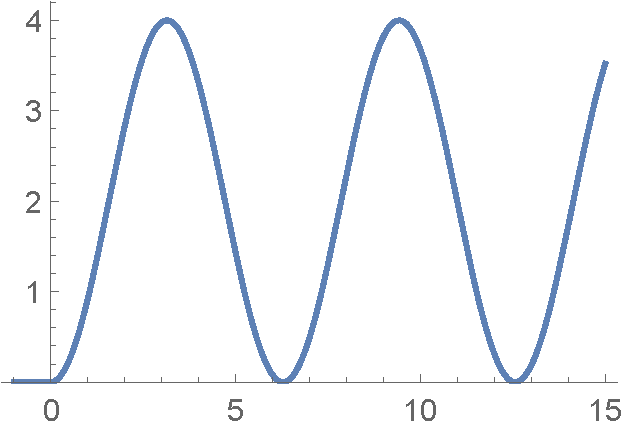
\includegraphics[width=5cm]{scal3-b}
				\end{center}
			\end{nota}
			Il \textbf{tempo di assestamento} associato all'esponenziale convergente può dunque essere calcolato e dipende solamente dalla parte reale del polo; in analogia al caso di polo unico puramente reale il tempo di assestamento viene calcolato come
			\begin{equation}
				t_a = \frac 5 {\xi \omega} = \frac 5 {\textrm{Re}}
			\end{equation}
			
		\subsubsection{Zero reale nell'origine}
			Fino ad ora si è osservato l'effetto che la posizione dei poli ha nel calcolo delle caratteristiche salienti delle funzioni di trasferimento di sistemi lineari: si vuole analizzare ora invece come gli zeri influenzano la risposta (anche se le considerazioni che trarremo non saranno a carattere generale come nel caso dell'analisi dei poli).
			
			Considerando un primo esempio di funzione di trasferimento con zero reale nell'origine, ossia di tipo $g = -1$, e con un solo polo stabile (con costante di tempo $T>0$) allora $G(s)$ può essere espressa come
			\[ G(s) = \frac{\mu s}{Ts+1} \qquad \xrightarrow[\textrm{scalino}]{\textrm{risposta allo}} \quad Y(s) = G(s) U(s) = \frac \mu {Ts+1} \]
			Applicando il teorema del valore iniziale si osserva che lo stesso non parte più da un valore nullo, ma dal valore $y_0 = \mu/T$; anche il valore finale, tramite l'utilizzo del relativo teorema, si dimostra essere diverso dai casi precedenti e convergente al valore $y_\infty = 0$; questo fatto può essere intuitivamente dimostrato considerando che il polo nell'origine $s$ coincide con l'operatore derivata (eq. \ref{eq:class:derivata}, pag. \pageref{eq:class:derivata}): derivando la risposta ad un polo (figura \ref{scal1-b}) e osservando che la stessa tende asintoticamente ad una costante, allora la sua derivata è nulla. 
			\begin{concetto}
				L'effetto generale di introdurre un zero nell'origine è quello di annullare la risposta asintotica del sistema.
			\end{concetto}
			Anti-trasformando l'uscita con il metodo di Heaviside è possibile calcolare la risposta del sistema nel dominio del tempo secondo l'espressione
			\[ y(t) = \anti{\frac{\mu s}{(Ts+1)s}} = \frac \mu T e^{-t/T} \]
			Facendo riferimento alla rappresentazione dell'uscita in figura \ref{scal4-a} è possibile osservare come lo zero non cambi le proprietà del transitorio: in particolare esso è determinato ancora dalle caratteristiche del polo a parte reale negativa e dunque con tempo di assestamento $t_a = 5T$.
			
			
			\figura{5}{1}{scal4-a}{risposta allo scalino di una funzione di trasferimento del tipo $\frac{\mu s}{Ts+1}$ con guadagno $\mu = 2$ e costante di tempo $T=2$.}{scal4-a}
			
		\subsubsection{Zero reale non nell'origine}
			Si consideri una funzione di trasferimento del primo ordine con polo a parte reale negativa ($T>0$ per garantire l'asintotica stabilità del sistema) e con uno zero con costante di tempo $\tau \neq 0$ (in questo caso non è necessario imporre il \textit{segno} della posizione del polo in quanto non appartiene alle specifiche dei criteri di stabilità) e dunque nella forma
			\[ G(s) = \mu \frac{\tau s + 1}{Ts+1}  \qquad \xrightarrow[\textrm{scalino}]{\textrm{risposta allo}} \quad Y(s) = G(s) U(s) = \mu \frac{\tau s + 1}{s(Ts+1)}\]
			A questo punto dall'analisi dei teoremi del valore iniziale e finale è possibile calcolare sia il valore iniziale, che risulta valere $y_0  \mu \tau/T$, che il valore asintotico $y_\infty =\mu$ (che torna dunque a coincidere con il guadagno della funzione di trasferimento). Anti-trasformando con Heaviside si ottiene dunque la funzione $y$  pari a 
			\[y(t) = \anti{\mu \frac{\tau s + 1}{s(Ts+1)}} = \mu \left(1 + \frac{\tau - T}T e^{-t/T}\right)  \]
			Anche in questo caso gli zeri reali non influiscono sul transitorio (il cui tempo di assestamento è determinato dal polo e dunque $t_a = 5T$), tuttavia è possibile osservare come la costante di tempo $\tau$ cambia il valore iniziale $y_0$ dell'uscita: in particolare per $\tau <0$ (zero a parte reale positiva) l'uscita parte da un valore negativo, per $0<\tau<T$ l'uscita parte da un valore compreso tra 0 e $\mu$ mentre per $\tau > T$ il valore iniziale $y_0$ è maggiore del guadagno e si ha dunque un fenomeno di sovra-elongazione (figura \ref{fig:lti:sist1zero}).
			
			\begin{figure}[bht]
				\centering
				\begin{subfigure}{0.325\linewidth}
					\centering
					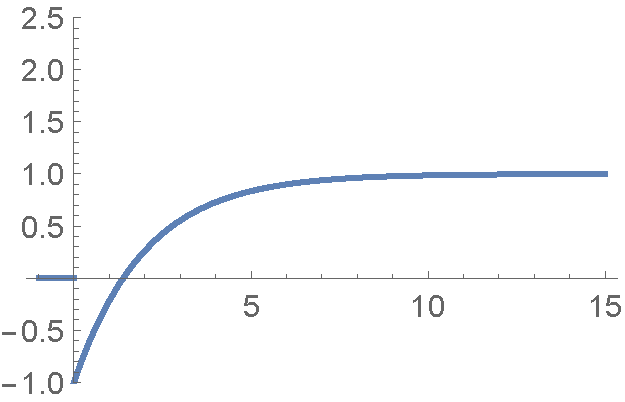
\includegraphics[width=4cm]{scal4-b} \caption{}
				\end{subfigure}
				\begin{subfigure}{0.325\linewidth}
					\centering
					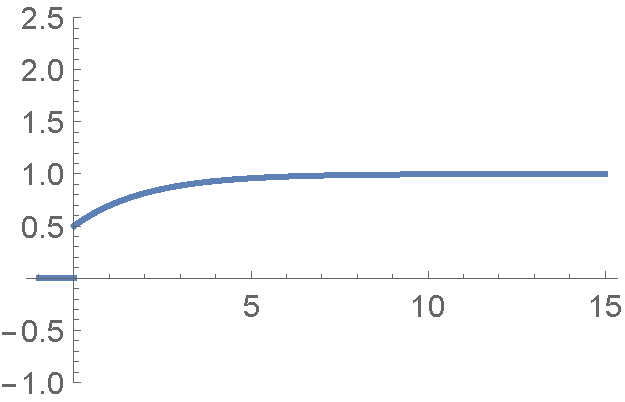
\includegraphics[width=4cm]{scal4-c} \caption{}
				\end{subfigure}
				\begin{subfigure}{0.325\linewidth}
					\centering
					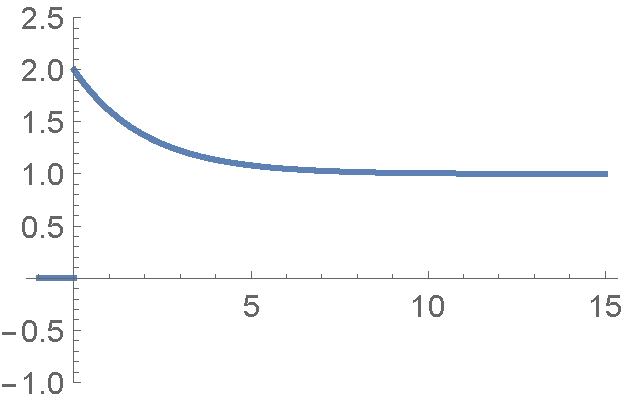
\includegraphics[width=4cm]{scal4-d} \caption{}
				\end{subfigure}
				\caption{risposta allo scalino di una funzione di trasferimento del tipo $\mu \frac{\tau s + 1}{Ts+1}$ con guadagno $\mu = 1$, costante di tempo $T=2$ e costanti di tempo degli zeri che cambiano: $\tau = -2$ (a), $\tau = 1$ (b) e $\tau = 4$ (c).} 
				\label{fig:lti:sist1zero}
			\end{figure}
		
		\subsubsection{Sistemi di ordine 2 con uno zero}
			Si consideri il sistema asintoticamente stabile ($T_1,T_2>0$) con zero non nell'origine la cui funzione di trasferimento vale
			\[ G(s) = \mu \frac{\tau s + 1}{\big(T_1s +1\big)\big(T_2s+1\big)} \qquad \xrightarrow[\textrm{scalino}]{\textrm{risposta allo}} \quad Y(s) = \mu \frac{\tau s + 1}{s\big(T_1s +1\big)\big(T_2s+1\big)} \]
			Dall'analisi tramite i teoremi del valore iniziale e finale si conclude che $y_0=0$ mentre $\dot y_0 = \mu \dfrac{\tau}{T_1T_2}$, mentre l'uscita asintotica rimane pari al guadagno $y_\infty = \mu$.
			\begin{concetto}
				A livello generale l'ordine della prima derivata di $y(t)$ non nulla nell'origine dei tempi coincide con il grado relativo della funzione di trasferimento, ossia tra la differenza del numero di poli e il numero di zeri di $G(s)$.
			\end{concetto}
			
			Anti-trasformando con il metodo di Heaviside è dunque possibile stabilire l'uscita in funzione del tempo:
			\[ y(t) = \anti{\mu \frac{\tau s + 1}{s\big(T_1s +1\big)\big(T_2s+1\big)}} = \mu \left( 1 - \frac{T_1-\tau}{T_1-T_2} e^{-t/T_1} + \frac{T_2-\tau}{T_1-T_2}e^{-t/T_2} \right) \]
			A livello intuitivo non è possibile capire quale sia il comportamento dell'uscita in funzione delle varie costanti di tempo $T_1,T_2,\tau$, tuttavia utilizzando i grafici (in figura \ref{fig:lti:sist2zero}, nella pagina seguente) è possibile osservare le seguenti proprietà:
			\begin{itemize}
				\item[a)] se lo zero è a parte reale positiva (ossia con $\tau <0$) allora si ha il fenomeno della cosiddetta \textbf{\textit{risposta inversa}} dove inizialmente l'uscita tende a valori negativi prima di riportarsi al valore del guadagno (più vicino è il polo dall'origine, più l'effetto sarà pronunciato);
				
				\item[b)] se lo zero è a parte reale negativa ma si trova più vicino all'origine dei poli (e dunque $\tau > T_1,T_2$) allora il sistema va incontro ad un fenomeno di sovra-elongazione che è tanto maggiore quanto più lo zero si avvicina all'origine dei numeri complessi;
				
				\item[c, d)] se lo zero determina una costante di tempo $\tau$ confrontabile con i valori $T_1,T_2$, allora l'effetto sarà quello di una \textit{cancellazione} e il comportamento viene approssimato ad una funzione di trasferimento ad un solo polo (complementare rispetto a quello cancellato);
				
				\item[e)] se lo zero ha una costante di tempo compresa tra quella dei poli ($T_2 < \tau < T_1$) allora il comportamento dell'uscita sarà compresa tra la risposte dei sistemi a un solo polo reale con costanti $T_1$ e $T_2$ rispettivamente;
				
				\item[f)] se lo zero si trova più \textit{lontano rispetto all'origine} dei poli (ossia per $\tau < T_1,T_2$) allora il comportamento dell'uscita convergerà al caso di una funzione a due poli reali in $T_1,T_2$ (senza effetto del polo).
				
			\end{itemize}
			
			\begin{figure}[p]
				\centering
				\begin{subfigure}{0.48\linewidth}
					\centering
					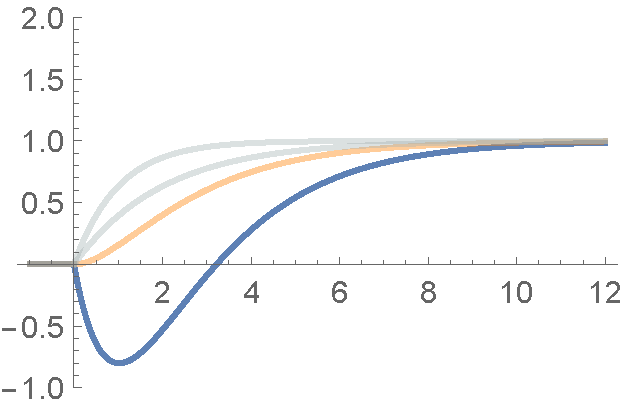
\includegraphics[width=6cm]{scal5-a} \caption{}
				\end{subfigure}
				\begin{subfigure}{0.48\linewidth}
					\centering
					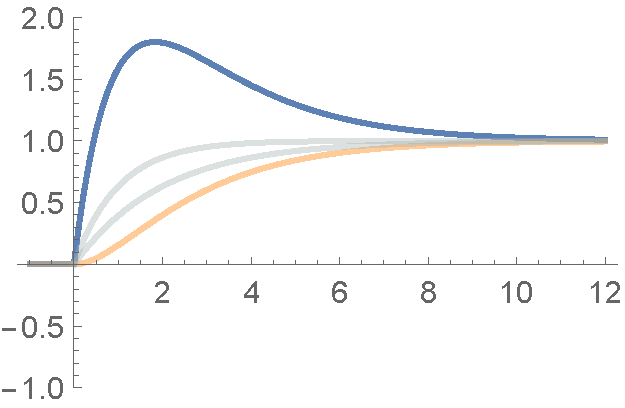
\includegraphics[width=6cm]{scal5-b} \caption{}
				\end{subfigure}
				\begin{subfigure}{0.48\linewidth}
					\centering
					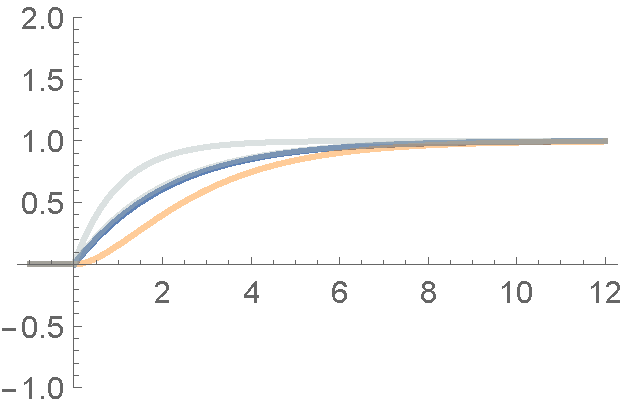
\includegraphics[width=6cm]{scal5-c} \caption{}
				\end{subfigure}
				\begin{subfigure}{0.48\linewidth}
					\centering
					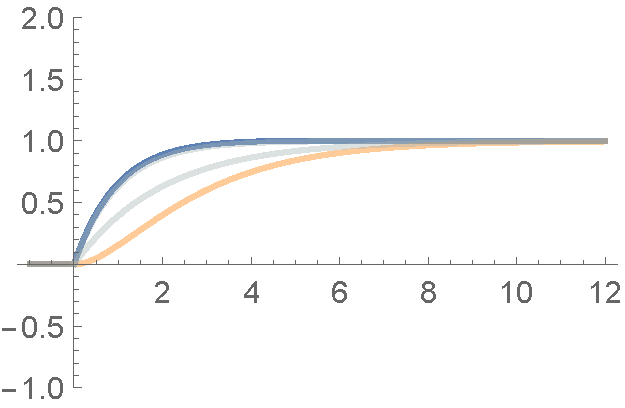
\includegraphics[width=6cm]{scal5-d} \caption{}
				\end{subfigure}
				\begin{subfigure}{0.48\linewidth}
					\centering
					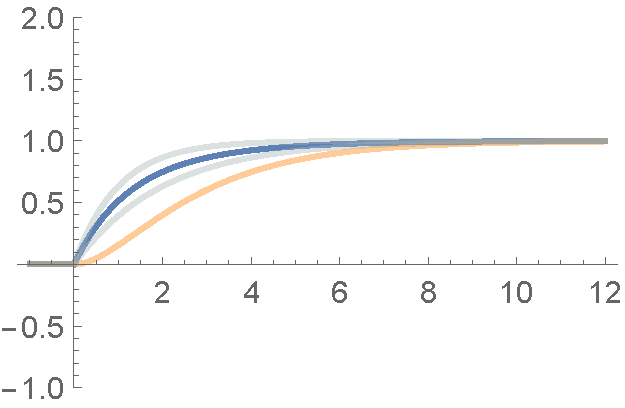
\includegraphics[width=6cm]{scal5-e} \caption{}
				\end{subfigure}
				\begin{subfigure}{0.48\linewidth}
					\centering
					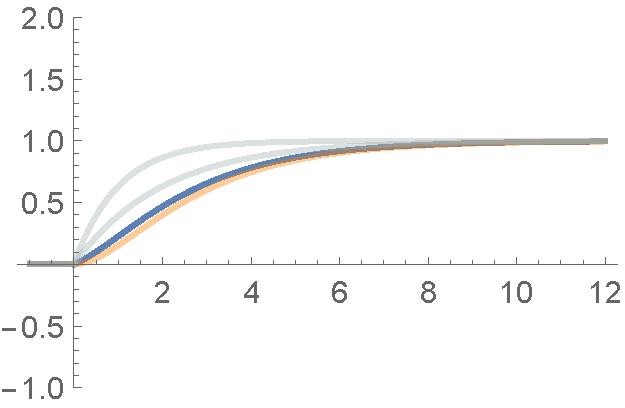
\includegraphics[width=6cm]{scal5-f} \caption{}
				\end{subfigure}
			
				\caption{risposta allo scalino di una funzione di trasferimento del tipo $\mu \frac{\tau s + 1}{(T_1s+1)(T_2s+1)}$ con guadagno $\mu = 1$, costanti di tempo $T_1 = 2$ e $T_1 = 1$. In arancione è mostrato il comportamento della funzione composta dai soli poli reali, mentre in grigio è mostrata la risposta dei sistemi ad un solo polo (di costanti $T_1$ e $T_2$ rispettivamente). In blu sono mostrate le risposte per valori $\tau = -4$ (a) cui è associato il fenomeno della risposta inversa, $\tau = 6$ (b) cui è associato il fenomeno della sovra-elongazione, $\tau = 0.9 \approx T_2$ (c) e  $\tau = 2.1 \approx T_1$ (d) cui è associato l'effetto di cancellazione, $\tau=1.5$ (e) e $\tau =0.3$ (f).}
				\label{fig:lti:sist2zero}
			\end{figure}
		
		\subsubsection{Effetto degli zeri sulla risposta allo scalino}
			A questo punto è possibile riassumere in maniera sintetica gli effetti che l'aggiunta degli zeri provoca sul sistema, in particolare:
			\begin{itemize}
				\item zeri nell'origine ($G(s)$ con tipo $g\leq -1$) annullano la risposta asintotica del sistema (considerando che la stessa sia pari ad una costante);
				\item gli zeri \textit{destri} (a parte reale positiva) determinano il fenomeno della risposta inversa, mentre gli zeri vicini all'asse immaginario determinano un fenomeno di sovra-elongazione;
				\item gli zeri vicini ad un polo tendono a \textit{mascherarne} l'effetto, ossia come se vi fosse una cancellazione critica nel sistema;
				\item gli zeri tendono a \textit{velocizzare} la risposta iniziale (che come visto dipende dal grado relativo tra polinomio a denominatore e numeratore).				
			\end{itemize}
			In generale gli zeri hanno un effetto sulla risposta allo scalino del sistema che non è facile da predire, che non è notevole e per le quali è difficile trovare delle soluzioni analitiche.
			
		\subsubsection{Risposta allo scalino di sistemi arbitrariamente complessi}
			In generale un sistema lineare ha una funzione di trasferimento che presenta numerosi contributi di zeri e poli sia reali che complessi coniugati (come visto nelle possibili rappresentazioni nell'equazione \ref{eq:lti:parametrizzazione}, \pageref{eq:lti:parametrizzazione}):
			\[ G(s) = \frac \mu {s^g} \frac{\prod\big(\textrm{zeri reali}\big) \prod \big(\textrm{zeri complessi coniugati}\big)}{\prod\big(\textrm{poli reali}\big) \prod \big(\textrm{poli complessi coniugati}\big)} \]
			
			Come visto analizzando gli effetti degli zeri, definendo il parametro $r$ come il grado relativo del polinomio a denominatore rispetto quella a numeratore al quale viene sottratto il valore unitario, allora si dimostra che
			\[ r = \textrm{grado relativo} - 1 \qquad \Rightarrow \quad y_0,\dot y_0 ,\dots, y_0^{(r)} = 0 \]
			Se il  sistema è asintoticamente stabile allora il valore asintotico coincide con il guadagno  ($y_\infty = \mu$) tranne nel caso in cui si hanno presenti zeri nell'origine dove la risposta si annulla (quindi se $g\leq -1$ allora $y_\infty = 0$). \\
			\begin{concetto}
				Per quanto riguarda le caratteristiche transitorie si può approssimare l'uscita considerando solamente le caratteristiche di \textbf{poli} e \textbf{zeri dominanti}, ossia le singolarità cui sono associati dei transitori più lenti (costanti di tempo maggiori e dunque poli/zeri più vicini all'asse dei numeri immaginari):
				\[ t_a = \frac{5}{\left|\textrm{Re}_\textrm{polo dominante}\right|} \qquad T = \frac{2\pi}{\textrm{Im}_\textrm{polo dominante}} \]
			\end{concetto}
			\begin{osservazione}
				Se un polo e uno zero sono molto vicini tra loro, allora vige l'\textit{idea} della cancellazione del polo con lo zero e dunque non si considerano gli effetti di tali singolarità.
			\end{osservazione}
			
	\subsection{Risposta alla sinusoide: analisi nel dominio della frequenza}
		Studiare la risposta di un sistema con funzione di trasferimento $G(s)$ rispetto ad un ingresso sinusoidale è utile per studiare la risposta in frequenza del sistema. In questo caso, essendo il sistema lineare, ci si aspetta che l'uscita sia anch'essa una sinusoide: questo significa che non è possibile applicare il teorema \ref{teor:valfinale} del valore finale (pag. \pageref{teor:valfinale}) per calcolare l'uscita asintotica del sistema, ma per questo è necessario introdurre il \textbf{teorema della risposta in frequenza}.
		
		\begin{teorema}{ teorema della risposta in frequenza \label{teor:rispostafrequenza} }
				\texttt{Ipotesi:} Questo teorema può essere applicato ad una funzione di trasferimento $G(s)$ solo se essa è razionale con poli a parte reale negativa (o eventualmente immaginari con parte reale nulla), ossia per un sistema che risulta essere asintoticamente stabile. 
				
				\vspace{3mm}
				
				\texttt{Enunciato:} {\itshape Dato un sistema lineare tempo invariante con funzione di trasferimento $G(s)$ (rispetto alla quale valgono le ipotesi) soggetto ad un ingresso sinusoidale di ampiezza $A$, pulsazione $\overline \omega$ e fase $\phi$ del tipo
				\[  u(t) = A \sin\big(\overline \omega t + \phi\big)\]
				allora l'uscita asintotica del sistema, espressa nel dominio del tempo, può essere valutata tramite la relazione
				\begin{equation}
					y_\infty(t) = A \big|G(i\overline \omega)\big| \sin \big(\overline \omega t + \phi + \angle G(i\overline \omega)\big)
				\end{equation}
				dove $\big|G(i\overline \omega)\big|$ rappresenta il \textbf{modulo} della funzione di trasferimento valutata per la pulsazione $\overline \omega$, mentre $ \angle G(i\overline \omega)$ rappresenta lo \textbf{sfasamento} dovuto alla funzione di trasferimento. 			}
		\end{teorema} 
		\begin{osservazione}
			Si osserva che per sistemi lineari tempo invarianti la pulsazione del segnale d'uscita è dunque pari a quella del segnale in ingresso: questo infatti non è necessariamente vero per le altre classi di sistemi!
			
			L'ampiezza del segnale in uscita in particolare risulta essere amplificata/ridotta in funzione del modulo della funzione di trasferimento; $G(s)$ introduce inoltre uno sfasamento tra ingresso e uscita.
		\end{osservazione}
		Va notato che il modulo e lo sfasamento introdotto dalla funzione di trasferimento non sono dei termini costanti, ma sono strettamente correlati al valore della pulsazione $\overline \omega$ rispetto alla quale si effettua il \textit{test}. In particolare per calcolare i valori di modulo e fase è necessario sostituire alla variabile $s$ nella funzione di trasferimento il numero immaginario $i\overline \omega$ e valutare (a partire da tale sostituzione) il modulo e fase.
		
		\begin{esempio}{: funzione di trasferimento nel dominio della frequenza}
			Considerando per esempio la funzione di trasferimento $G(s) = \frac 1 {s+2}$, allora essa può essere espressa nel dominio della frequenza sostituendo ad $s$ il numero puramente immaginario $i\omega$ e, tramite manipolazione algebrica, separare parte reale e immaginaria:
			\[ G(i\omega) = \frac 1 {i\omega + 2} = \frac{2-i\omega}{(2+i\omega)(2-i\omega)} = \underbrace{\frac{2}{4+\omega^2}}_\textrm{Re} - i \underbrace{\frac \omega {4+\omega^2}}_\textrm{Im} \]
		\end{esempio}
		
		\vspace{3mm}
		
		Il teorema del valore finale permette solamente di determinare la risposta asintotica di un segnale sottoposto ad ingresso sinusoidale, mentre la parte transitoria (e in particolare il tempo di assestamento) viene valutato in maniere alternative, in particolare resta valida l'\textit{idea} di calcolare tale proprietà considerando la parte reale dei poli dominanti $t_a =  5 /\left|\textrm{Re}_\textrm{p.dom.}\right|$.
		
		\paragraph{Importanza della risposta in frequenza} Analizzare la risposta in frequenza di un sistema dinamico è molto importante; considerando infatti la teoria sviluppata da Teoria, ogni ingresso $u(t)$ di periodo $T$ (per segnali aperiodici si può considerare $T\rightarrow \infty$ ed estendere la sommatoria ad un integrale) può essere rappresentato tramite la cosiddetta \textbf{serie di Fourier} per cui
		\[ u(t) = \sum_{k=0}^\infty H\big(\omega_k\big) \sin\big(\omega_k t + \phi(\omega_k)\big) \qquad \textrm{con } \omega_k = k \frac{2\pi}{T} \]
		dove sia l'ampiezza $H(\omega)$ che lo sfasamento $\phi(\omega)$ sono dei coefficienti che possono essere determinati.
		
		Scomponendo dunque con Fourier un ingresso generico allora l'uscita asintotica del sistema può essere calcolata sfruttando anche il teorema della risposta in frequenza, e dunque
		\begin{equation} \label{eq:lti:fourier}
			y_\infty(t) = \sum_{k=0}^\infty \Big[ H(\omega_k) \, \big|G(i\omega_k)\big| \sin\Big(\omega_kt + \phi(\omega_k) + \angle G(i\omega_k)\Big) \Big]
		\end{equation}
		Essendo il sistema lineare per determinare l'uscita di un generico ingresso è sufficiente analizzare la trasformata di ogni singola armonica sinusoidale che compone l'ingresso e poi sommare ogni contributo. Il \textbf{modulo} $H(\omega)$ (definito positivo) e la \textbf{fase} $\phi(\omega)$ presenti nell'equazione \ref{eq:lti:fourier} rappresentano lo \textbf{spettro del segnale} associato all'ingresso generico $u(t)$ nel dominio della frequenza.
			
		Di particolare interesse pratico è l'analisi del modulo $H(\omega)$ del segnale in ingresso: per esempio se lo stesso assume valori \textit{importanti} a frequenze elevate significa che l'ingresso $u(t)$ associato sarà molto \textit{rumoroso}, in quanto presenta grandi oscillazioni a frequenze alte; al contrario un segnale che dopo una certa frequenza $\omega^*$ (non troppo elevata) presenta modulo $H(\omega)$ basso/nullo può essere associato ad un ingresso $u(t)$ sufficientemente \textit{continuo} e senza molti picchi/disturbi.
			
		\vspace{3mm}
		
		\begin{concetto}
			L'applicazione del teorema della risposta in frequenza dunque permette di analizzare ancora più nel dettaglio la risposta a ingressi sinusoidali generici del sistema. Nota la scrittura  in forma matriciale della rappresentazione di stato di un sistema lineare tempo invariante è possibile infatti determinare la funzione di trasferimento $G(s)$ nel dominio di Laplace: a questo punto analizzando $G$ nel dominio della frequenza è possibile analizzare la \textbf{risposta in frequenza di un sistema dinamico}, determinando una funzione complessa $G(i\omega)$ dipendente dal parametro $\omega$.
		\end{concetto}
		
		Essendo questa funzione complessa essa può essere analizzata o tramite scomposizione in parte reale e immaginaria, oppure, come si preferisce, analizzando modulo $|G(i\omega)|$ e fase $\angle G(i\omega)$ della funzione di trasferimento. Le principali rappresentazioni delle funzioni di trasferimento nel dominio della frequenza sono determinate dai \textbf{diagrammi di Bode} e dai \textbf{diagrammi polari}.
			
			
		\begin{figure}[bht]
			\centering
			\begin{subfigure}{0.48\linewidth}
				\centering 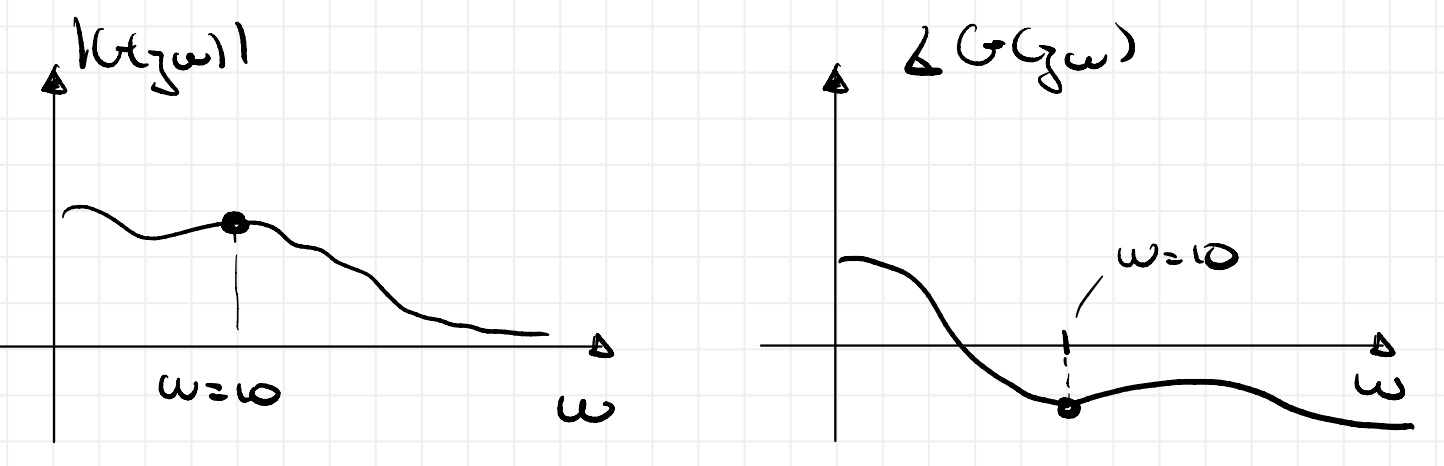
\includegraphics[width=6cm]{bode} \caption{}
			\end{subfigure}
			\begin{subfigure}{0.48\linewidth}
				\centering 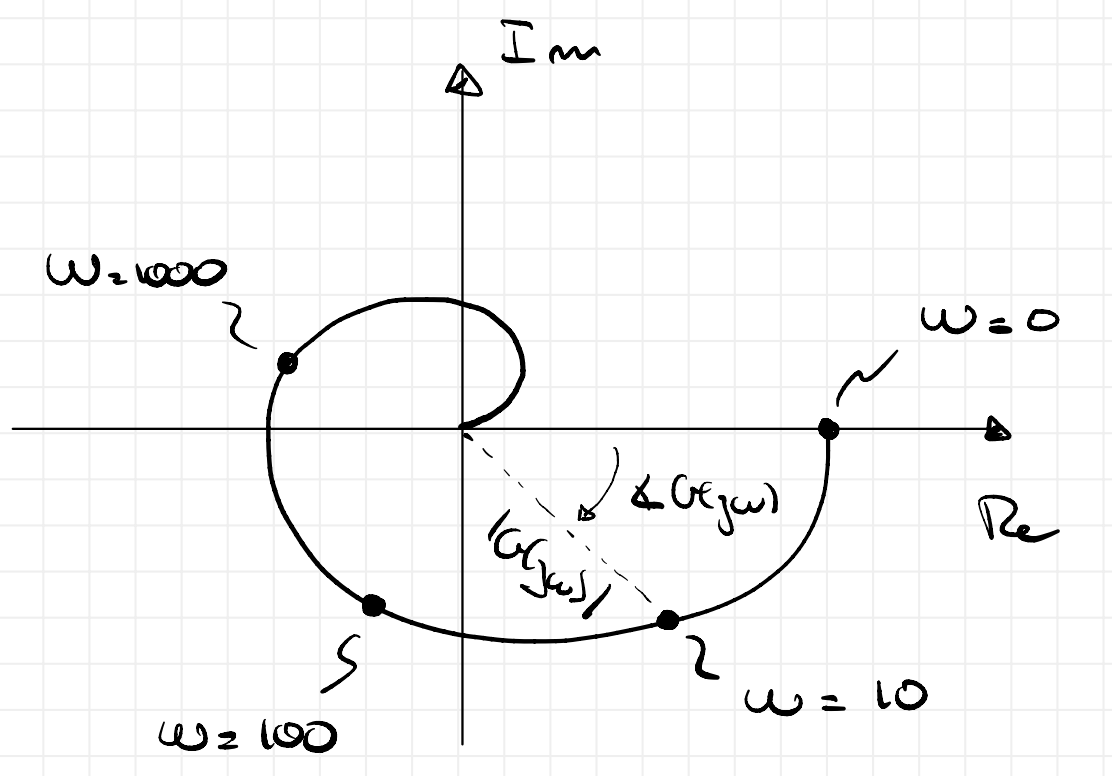
\includegraphics[width=5.5cm]{nyquist} \caption{}
			\end{subfigure}
			\caption{esempi di rappresentazione di una funzione di trasferimento $G(i\omega)$ nel dominio della frequenza secondo i diagrammi di Bode (a) con modulo e fase oppure tramite diagramma polare (b).}
			\label{fig:lti:bodenyquist}
		\end{figure}
		
		
	\subsection{Diagrammi di Bode}
		Per poter analizzare in modo efficace la risposta in frequenza di un sistema dinamico lineare è necessario capire come rappresentare correttamente i diagrammi di $G(s)$; la rappresentazione più \textit{facile} e \textit{comoda} da determinare è quella di Bode.
		
		Questo tipo di diagrammi sono caratterizzati da un'asse delle ascisse non in scala lineare, ma in scala semi-logaritmica in base 10: questo significa che \textit{spostandosi} di un valore unitario nell'asse orizzontale del diagramma, si trova una pulsazione $\omega$ 10 vole più grande: per questo si parla spesso di \textbf{\textit{decadi}}. Si osserva inoltre che associata all'ascissa nulla non corrisponde la pulsazione nulla $\omega=0$, ma $\omega = \log_{10}(0) = 1$: per trovare la pulsazione nulla è necessario spostarsi infinitamente verso sinistra nel diagramma.
		
		Il modulo della funzione di trasferimento $G$ non viene misurato in \textit{unità}, ma in \textit{decibel} $dB$. La conversione tra grandezze scalari e decibel è data dalla relazione
		\[ |G(i\omega)|_{dB} = 20 \log_{10} |G(i\omega)| \qquad \Leftrightarrow \qquad |G(i\omega)| = 10 ^{|G(i\omega)|_{dB}/20}  \]
		
		Determinare i diagrammi di Bode reali di funzioni di trasferimento non è mai in generale facile, per questo si fa spesso riferimento ai \textbf{diagrammi di Bode asintotici} che sono caratterizzati dalla presenza di sole rette e spezzate. I diagrammi sono detti \textit{asintotici} in quanto trascurano il comportamento di $G(i\omega)$ nell'intorno degli zeri e dei poli, ma determina un andamento qualitativo al di fuori di tali valori.
		
		\paragraph{Rappresentazione del diagramma del modulo} I diagrammi di Bode sono caratterizzati  dai grafici di modulo e fase. Analizzando ora il primo di questi diagrammi, si osserva che lo smorzamento di poli e zeri complessi coniugati non influenza il tracciamento del comportamento asintotico: questa situazione infatti può essere ricondotta a due poli o zeri a parte reale coincidente. Questo significa che di poli e zeri si deve sempre considerare la parte reale, e non quella immaginaria. Si osserva inoltre che il comportamento di poli e zeri nel diagramma di Bode è uguale a meno di un segno.
		
		In linea generale per tracciare i diagrammi di Bode della funzioni di trasferimento (fattorizzate nella forma di Bode, eq. \ref{eq:lti:parametrizzazione}, pag. \pageref{eq:lti:parametrizzazione}) è possibile procedere con i seguenti passaggi:
		\begin{enumerate}
			\item avendo determinato i parametri $\mu,,T,\tau,\omega,\alpha$ della funzione di trasferimento, si parte a tracciare il grafico \textit{da sinistra}, ossia per pulsazioni $\omega$ che tendono al valore nullo. In particolare si parte stabilendo il contributo dovuto a guadagno $\mu$ e tipo $g$ della funzione di trasferimento: esso è associato ad una retta la cui pendenza e intercetta $\overline \omega$ con l'asse a zero decibel vale
			\[ \textrm{pendenza: } -20 g \ \frac{dB}{dec} \qquad \overline \omega = |\mu|^{1/g}_{dB} \]
			\begin{center}
				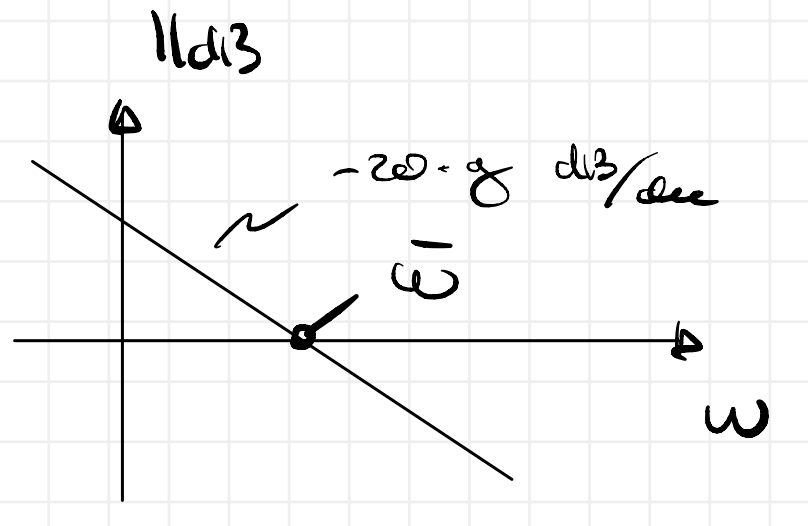
\includegraphics[width=4cm]{bode-a}
			\end{center}
			Nel caso particolare in cui il tipo $g$ sia  nullo, allora la retta è orizzontale e intercetta l'asse del modulo (in decibel) al valore del guadagno in decibel.
			\begin{center}
				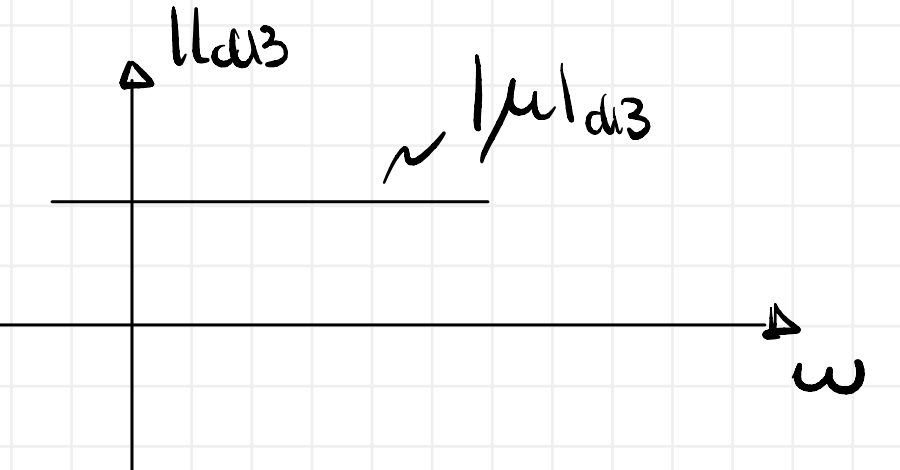
\includegraphics[width=4cm]{bode-b}
			\end{center}
			
			\item a questo punto è necessario determinare le pulsazioni angolari associate ai poli $\omega_r$ e agli zeri $\omega_z$, siano essi reali (pedice $r$) o complessi coniugati (pedice $cc$), tramite le relazioni
			\[ \omega_{p,r} = \frac 1 {|T|} \qquad \omega_{p,cc} = \omega \qquad \omega_{z,r} = \frac 1 {|\tau|} \qquad \omega_{z,cc} = \alpha \]
			
			\item in corrispondenza delle pulsazioni trovate, \textit{andando da sinistra verso destra}, si modifica la retta iniziale nel seguente modo: in corrispondenza di un polo la pendenza della retta della caratteristica statica subisce una diminuzione pari a $-20dB/dec$, mentre in caso di poli complessi coniugati (due poli singoli sovrapposta) la variazione di pendenza associata è di $-40dB/dec$. Al contrario incontrando uno zero reale è necessario aumentare la pendenza di $20dB/dec$, in presenza di uno zero complesso coniugato invece la pendenza aumenta di $40dB/dec$.
			
		\end{enumerate}
			
			
			
			
			
			
			
			
	
		
		
	
	
\end{document}